\documentclass
  [ acmsmall
  , xetex
  , dvipsnames
  % , review
  , nonacm
  , screen
  % , authordraft
  ]{acmart}

% framist 翻译中... 由 ChatGP 与 DeepL 赋能
% ChatGP prompt: 请翻译以下文本到中文,保留 latex 的格式,中英文之间添加空格,适当换行避免一行过长,将输出放在代码框中。不要画蛇添足,你只需翻译我输入的内容。


\usepackage{xeCJK} % 中文支持
\usepackage{fontspec}
\setmonofont[Mapping=tex-text]{Inconsolata} % 修复 mono bug
\setlength{\parindent}{2em} %首行二字符缩进
% \linespread{1.1} % 行距

\usepackage{hyperref}

\authorsaddresses{}
\setcopyright{none}
\settopmatter{
  printfolios=true,
  printccs=false,
  printacmref=false
}

\bibliographystyle{ACM-Reference-Format}
\citestyle{acmauthoryear}

\usepackage{graphics}
\graphicspath{{_build/}{fig/}}

\makeatletter
\def\@ACM@badge@width{8mm}
\makeatother
\acmBadgeL{egg.png}


% \title{\egg: Fast and Extensible Equality Saturation}
\title{\egg: 快速和可拓展的等式饱和}
% \egg: 快速和可拓展的等式饱和

\usepackage{xspace}
\usepackage{xargs}
\usepackage[
  colorinlistoftodos,
  prependcaption,
  % disable,
]{todonotes}
\usepackage{fontenc}


\usepackage{subcaption}

% \usepackage{hyperref}
\def\sectionautorefname{Section}
\def\subsectionautorefname{Section}
\def\subsubsectionautorefname{Section}

\usepackage{listings}
\lstset{
  columns=flexible,
  keepspaces=true,
  showstringspaces=false,
  stringstyle=\slshape\color{green!40!black},
  basicstyle=\ttfamily\small,
  language=Python,
  morekeywords={*, self},
  commentstyle=\slshape\color{black!60},
  tabsize=2,
}

\lstdefinelanguage{Rust}{
  sensitive,
  morecomment=[l]{//},
  morecomment=[s]{/*}{*/},
  moredelim=[s][{\itshape\color[rgb]{0,0,0.75}}]{\#[}{]},
  morestring=[b]{"},
  alsodigit={},
  alsoother={},
  alsoletter={!},
  % keywords
  otherkeywords={=>},
  morekeywords={break, continue, else, for, if, in, loop, match, return, while},
  morekeywords={as, const, let, move, mut, ref, static, unsafe},
  morekeywords={dyn, enum, fn, impl, Self, self, struct, trait, type, use, where},
  morekeywords={crate, extern, mod, pub, super},
  morekeywords={abstract, alignof, become, box, do, final, macro,
    offsetof, override, priv, proc, pure, sizeof, typeof, unsized, virtual, yield},
  % traits
  morekeywords=[2]{Send},
  % types
  morekeywords=[3]{bool, char, f32, f64, i8, i16, i32, i64, isize, str, u8, u16, u32, u64, unit, usize, i128, u128},
}%


\author{Max Willsey}
\affiliation{\institution{University of Washington, Seattle} \country{USA}}
\author{Chandrakana Nandi}
\affiliation{\institution{University of Washington, Seattle} \country{USA}}
\author{Yisu Remy Wang}
\affiliation{\institution{University of Washington, Seattle} \country{USA}}
\author{Oliver Flatt}
\affiliation{\institution{University of Utah, Salt Lake City} \country{USA}}
\author{Zachary Tatlock}
\affiliation{\institution{University of Washington, Seattle} \country{USA}}
\author{Pavel Panchekha}
\affiliation{\institution{University of Utah, Salt Lake City} \country{USA}}

\newcommand{\missing}[1]{{\color{red}\bfseries [TODO]}}

\newcommand{\egg}{\texorpdfstring{\MakeLowercase{\texttt{egg}}}{\texttt{egg}}\xspace}
\newcommand{\Egg}{\texorpdfstring{\MakeLowercase{\texttt{egg}}}{\texttt{egg}}\xspace}
% \newcommand{\egg}{Lego\xspace}
% \newcommand{\Egg}{Lego\xspace}
\newcommand{\egraphs}{\mbox{e-graphs}\xspace}
\newcommand{\egraph}{\mbox{e-graph}\xspace}
\newcommand{\Egraph}{\mbox{E-graph}\xspace}
\newcommand{\Egraphs}{\mbox{E-graphs}\xspace}
\newcommand{\eclass}{\mbox{e-class}\xspace}
\newcommand{\Eclass}{\mbox{E-class}\xspace}
\newcommand{\enode}{\mbox{e-node}\xspace}
\newcommand{\eclasses}{\mbox{e-classes}\xspace}
\newcommand{\enodes}{\mbox{e-nodes}\xspace}
\newcommand{\Enodes}{\mbox{E-nodes}\xspace}
% \newcommand{\regraph}{Regraph\xspace}
% \newcommand{\Regraph}{Regraph\xspace}
\newcommand{\sz}{Szalinski\xspace}
\newcommand{\find}{\texttt{find}\xspace}

\newcommand{\equivid}{\equiv_{\sf id}}
\newcommand{\equivnode}{\equiv_{\sf node}}
\newcommand{\equivterm}{\equiv_{\sf term}}

\newcommand{\congrinv}{$\mathcal{I}_c$\xspace}

\newcommand{\egglogo}[1][]{\protect
\includegraphics[height=1em, #1]{egg.png} }
\newcommand{\eggurl}{\url{https://github.com/mwillsey/egg}}

% TODOs
% https://tex.stackexchange.com/questions/9796/how-to-add-todo-notes

\newcommand{\eggtodo}[1]{\textcolor{Red}{\textbf{[CITE: #1]}}}

\newcommand{\defTodo}[2]{%
  \expandafter\newcommand\csname #1\endcsname[1]{%
    \todo[linecolor=#2,backgroundcolor=#2!25,bordercolor=#2,inline,size=\tiny]{\textbf{#1}: ##1}}}

\newcommand{\defTODO}[2]{%
  \expandafter\newcommand\csname #1\endcsname[1]{%
    \todo[linecolor=#2,backgroundcolor=#2!25,bordercolor=#2,inline,size=\tiny,caption={\textbf{(#1 LONG TODO)}}]{##1}}}

\newcommand{\LeoColor}{Goldenrod}
\newcommand{\MaxColor}{RoyalBlue}
\newcommand{\RemyColor}{Red}
\newcommand{\OliverColor}{OliveGreen}
\newcommand{\ChandraColor}{Magenta}
\newcommand{\PavelColor}{Cerulean}
\newcommand{\ZachColor}{Plum}
\newcommand{\BenColor}{Orchid}
\newcommand{\JamesColor}{Salmon}

\defTodo{Leo}{\LeoColor}
\defTodo{Max}{\MaxColor}
\defTodo{Remy}{\RemyColor}
\defTodo{Oliver}{\OliverColor}
\defTodo{Chandra}{\ChandraColor}
\defTodo{Pavel}{\PavelColor}
\defTodo{Zach}{\ZachColor}
\defTodo{Ben}{\BenColor}
\defTodo{James}{\JamesColor}

\defTODO{LEO}{\LeoColor}
\defTODO{MAX}{\MaxColor}
\defTODO{REMY}{\RemyColor}
\defTODO{OLIVER}{\OliverColor}
\defTODO{CHANDRA}{\ChandraColor}
\defTODO{PAVEL}{\PavelColor}
\defTODO{ZACH}{\ZachColor}
\defTODO{BEN}{\BenColor}
\defTODO{JAMES}{\JamesColor}

\newcommand{\CongrSpeedup}{\ensuremath{88\times}\xspace}
\newcommand{\TotalSpeedup}{\ensuremath{21\times}\xspace}
\newcommand{\RepairsR}{\ensuremath{0.98}\xspace}
\newcommand{\RepairsP}{3.6e-47\xspace}
\newcommand{\nEggTests}{32\xspace}
\newcommand{\nEggTimeouts}{8\xspace}


%%% Local Variables:
%%% TeX-master: "egg"
%%% End:

\newcommand{\HerbieOverallSpeedup}{\ensuremath{2.81\times}\xspace}
\newcommand{\HerbieSimplificationFractionBefore}{\ensuremath{45\%}\xspace}
\newcommand{\HerbieSimplificationFractionAfter}{\ensuremath{4.1\%}\xspace}


\begin{abstract}
  % 翻译完成
% 原文:
% An \egraph efficiently represents
%   a congruence relation over many expressions.
% Although they were originally developed in the late 1970s
%   for use in automated theorem provers,
%   a more recent technique known as \textit{equality saturation}
%   repurposes \egraphs to implement state-of-the-art,
%   rewrite-driven compiler optimizations and program synthesizers.
% However, \egraphs remain unspecialized for this newer use case.
% Equality saturation workloads exhibit distinct characteristics and
%   often require ad~hoc \egraph extensions to
%   incorporate transformations beyond purely syntactic rewrites.
一个 \egraph (e 图)可以有效地表示许多表达式上的同构关系。
虽然它最初是在 20 世纪 70 年代末为用于自动定理证明器而开发的,
  最近的一项技术被称为 \textit{等式饱和(equality saturation)}。
  重新利用了 \egraphs 来实现最先进的技术(SOTA),用于
  重写驱动的编译器优化和程序综合器(program synthesizers)。
然而,对于这种新的使用情况,\egraphs 仍然没有被专门化。
等式饱和的工作量表现出明显的特征,并且
  往往需要专门的 \egraph 扩展来纳入纯语法重写之外的转换。

% This work contributes two techniques that make
%   \egraphs fast and extensible, specializing them to equality saturation.
% A new amortized invariant restoration technique called \textit{rebuilding}
%   takes advantage of equality saturation's distinct workload,
%   providing asymptotic speedups over current techniques in practice.
% A general mechanism called \textit{\eclass analyses}
%   integrates domain-specific analyses into the \egraph,
%   reducing the need for ad hoc manipulation.
我们的工作提供了两项技术,使 \egraphs 快速和方便扩展,
  使其专门用于等式饱和。
一是新的摊销的不变性恢复技术,称为 \textit{重建(rebuilding)} 。
  利用了等式饱和的独特工作量。
  在实践中提供了比目前技术更多的渐进式加速(asymptotic speedups)。
二是一个名为 \textit{\eclass analyses} (e类分析)的通用机制,它
  将特定领域的分析整合到 \egraph 中,减少了临时操作的需要。         

% We implemented these techniques in
%   a new open-source library called \egg.
% Our case studies on
%   three previously published applications of equality saturation
%   highlight how \egg's performance and flexibility
%   enable state-of-the-art results across diverse domains.
我们将这些技术在一个新的开源库实现,叫做 \egg。
我们对以前发表的三个等式饱和的应用进行了案例研究,
  它突出了 \egg 的性能和灵活性,在不同的领域可达到最先进的效果。


%% --------------------------------------------------------------------------

%% \Egraphs are data structures originally developed in the 1970s
%%   for automated theorem provers to
%%   efficiently encode congruence relations over many expressions.
%% More recently, a technique known as \textit{equality saturation}
%%   has demonstrated promising results using \egraphs to implement
%%   rewrite-driven compiler optimizations and program synthesizers.
%% However, \egraphs have not been specialized to this use case.
%% Equality saturation workloads have distinct characteristics
%%   compared to the more general setting and
%%   often require \textit{ad hoc} extensions to
%%   incorporate transformations beyond syntactic rewrites.

%% In this work, we contribute two new techniques to make
%%   \egraphs fast and extensible for equality saturation.
%% We introduce \textit{rebuilding},
%%   a new, amortized algorithm for maintaining congruence closure
%%   that is specialized to the equality saturation workload,
%%   achieving super-linear speedups over current techniques in practice.
%% We also propose \textit{\eclass analyses},
%%   a general mechanism for integrating program analyses into the \egraph,
%%   reducing the need for \textit{ad hoc} manipulation.

%% We implemented these techniques in
%%   a new open-source library called \egg.
%% Our case studies on
%%   three previously published applications of equality saturation
%%   highlight how the flexibility of \eclass analysis
%%   supports diverse domains and
%%   how \egg can provide up to $3000\times$ speed ups.

%% --------------------------------------------------------------------------


%% An \egraph is a data structure originating from automated theorem provers that
%%   efficiently encodes a congruence relation over many expressions.
%% A more recent technique called \textit{equality saturation}
%%   achieves promising results
%%   using \egraphs to implement rewrite-driven compiler optimizations.
%% However, \egraphs ultimately remain better designed for their original use case.
%% Equality saturation implementations
%%   have not specialized \egraphs to a workload that is
%%   very different from that of theorem provers.
%% Users also frequently resort to \textit{ad hoc} manipulation to implement
%%   program analyses over the \egraph.
%% \Max{still not 100\% about the last sentence}

%% In this work, we contribute two new techniques to make equality saturation fast
%%   and extensible.
%% We introduce \textit{rebuilding}, a new, simpler algorithm for maintaining
%%   congruence closure that is specialized to the equality saturation workload,
%%   achieving an asymptotic speedup over current techniques.
%% We also propose \textit{\eclass analyses}, a general mechanism for
%%   integrating program analyses into the \egraph
%%   that can replace \textit{ad hoc} manipulation.

%% We realize these techniques in an open-source implementation called
%%   \egg, an easy, efficient, and extensible \egraph library.
%% With these contributions, we re-propose \egraphs and equality saturation as a
%%   solution to a diverse set of optimization and synthesis problems.
%% We highlight three applications in published works that rely on \egg's
%%   flexibility and speed to
%%   easily implement robust optimizers,
%%   add powerful analyses to them,
%%   and achieve up to $3000\times$ speed up.
%% \Max{still a little awkward, this sentence is saying a lot}



%%% Local Variables:
%%% TeX-master: "egg"
%%% End:

\end{abstract}

\begin{document}

\maketitle
\renewcommand{\shortauthors}{Willsey et al.}

% \listoftodos does not work with acmart by default
% https://groups.google.com/forum/#!topic/comp.text.tex/jiA1XWJc3ck
\makeatletter
\providecommand\@dotsep{5}
\makeatother

% If you have a multi-paragraph TODO, use the all-capitals version
% your TODO macro to avoid breaking the build (the \listoftodos above
% does not like paragraph breaks).
%
% Example:
%
%    \ZACH{%
%      This TODO has two parts after this brief introduction:
%
%      Here is the first part in one paragraph.
%
%      This is the second part in another paragraph.
%    }

\section{引入}
% Introduction
\label{sec:intro}

% 翻译完成

% Equality graphs (\egraphs) were originally developed to
%   efficiently represent congruence relations
%   in automated theorem provers (ATPs).
% At a high level, \egraphs~\cite{nelson, pp-congr}
%   extend union-find~\cite{unionfind} to compactly represent
%   equivalence classes of expressions while
%   maintaining a key invariant:
%   the equivalence relation is closed under congruence.\footnote{
%     Intuitively, congruence simply means
%     that $a \equiv b$ implies $f(a) \equiv f(b)$.} 
等价图(Equality graphs,即 \egraph)最初是为了
  在自动定理证明器(ATPs)中有效地表示同余(congruence)关系。
在高层次上, \egraphs~\cite{nelson, pp-congr} 
  扩展了并查集(union-find)~\cite{unionfind},用来紧凑地表示
  表达式的等价类,同时保持一个关键的不变性:
  等价关系在同余下是封闭的。\footnote{
    直观地说,同余简单的说就是
    $a \equiv b$ 蕴含 $f(a) \equiv f(b)$.}

    
% Over the past decade, several projects have repurposed \egraphs
%   to implement state-of-the-art, rewrite-driven
%   compiler optimizations and program synthesizers
%   using a technique known as \textit{equality saturation}~\cite{
%     denali, eqsat, eqsat-llvm, szalinski, yogo-pldi20, spores, herbie}.
% Given an input program $p$,
%   equality saturation constructs an \egraph $E$ that
%   represents a large set of programs equivalent to $p$,
%   and then extracts the ``best'' program from $E$.
% The \egraph is grown by repeatedly applying
%   pattern-based rewrites.
% Critically, these rewrites only add information to the \egraph,
%   eliminating the need for careful ordering.
% Upon reaching a fixed point (\textit{saturation}),
%   $E$ will represent \textit{all equivalent ways} to
%   express $p$ with respect to the given rewrites.
% After saturation (or timeout),
%   a final \textit{extraction} procedure
%   analyzes $E$ and selects the
%   optimal program according to
%   a user-provided cost function.
在过去的十年中,一些项目重新利用了 \egraphs
  来实现最先进的重写驱动的编译器优化和程序综合器。
  它们使用一种被称为 \textit{等式饱和}~\cite{
    denali, eqsat, eqsat-llvm, szalinski, yogo-pldi20, spores, herbie} 的技术。
给定一个输入程序 $p$ ,
   等式饱和 构建了一个 $E$ 图,它代表了一大批与之等价的程序。
  代表与 $p$ 等价的一大组程序。然后从 $E$ 中提取 "最好的 "程序。
该图增长是通过反复应用基于模式的重写。
最重要的是,这些改写只向 \egraph 增加信息。消除了对仔细排序的需要。
在达到一个不动点(\textit{饱和})时,
  $E$ 将代表 \textit{所有等价的方式} 来表达表达 $p$ 与给定重写的关系。
饱和(或超时)之后,最后的 \textit{萃取} (extraction)程序
  将分析 $E$ 并选择根据用户提供的成本函数,选择最佳程序。


% Ideally, a user could simply provide
%   a language grammar and rewrites,
%   and equality saturation would produce a effective optimizer.
% Two challenges block this ideal.
% First, maintaining congruence can become expensive as $E$ grows.
% In part, this is because \egraphs from the conventional ATP setting
%   remain unspecialized to the distinct \textit{equality saturation workload}.
% Second, many applications critically depend on
%   \textit{domain-specific analyses}, but
%   integrating them requires ad~hoc extensions to the \egraph.
% The lack of a general extension mechanism
%   has forced researchers to re-implement
%   equality saturation from scratch several times~\cite{herbie, eqsat, wu_siga19}.
% These challenges limit equality saturation's practicality.
理想情况下,用户可以简单地提供一个语言语法和一些重写规则。
  而 等式饱和 将产生一个有效的优化器。
但是有两个挑战阻碍了我们的期望:
首先,随着 $E$ 的增长,维持全等性会变得很昂贵(expensive)。
部分原因是传统 ATP(Automated Theorem Proving,自动定理证明)设置中的 \egraphs 
  仍然没有针对不同的 \textit{等式饱和工作负载(equality saturation workload)} 特化。
其次,许多应用关键性地依赖于 \textit{领域特定的分析(domain-specific analyses)},但是
  集成它们需要对 \egraph 进行特别的扩展。
由于缺乏一个通用的扩展机制迫使研究人员多次从头实现
  等式饱和~\cite{herbie, eqsat, wu_siga19}。
这些挑战限制了等式饱和的实用性。

% \textit{Equality Saturation Workload. $\,$}
% %
% ATPs frequently query and modify \egraphs and
%   additionally require \textit{backtracking} to
%   undo modifications (e.g., in  DPLL(T)~\cite{dpll}).
% These requirements force conventional \egraph designs
%   to maintain the congruence invariant after every operation.
% In contrast,
%   the equality saturation workload does not require backtracking and
%   can be factored into distinct phases of
%   (1) querying the \egraph to simultaneously find all rewrite matches and
%   (2) modifying the \egraph to merge in equivalences for all matched terms.
\textit{等式饱和工作负载. $\,$}
ATPs 经常查询和修改 \egraphs ,还需要对文本进行\textit{回溯(backtracking)}
  来撤销修改(例如在 DPLL(T)~\cite{dpll} 中)。
这些要求迫使传统的 \egraph 设计为在每次操作后都要保持同余不变性。
与此相反,
  等式饱和工作负载不需要回溯,并且可以被分解为以下不同的阶段:
  (1) 查询 \egraph 以同时找到所有的重写匹配
  (2) 修改 \egraph 以合并所有匹配术语的等价关系。

% We present a new amortized algorithm
%   called \textit{rebuilding} that defers \egraph invariant maintenance
%   to equality saturation phase boundaries without compromising soundness.
% Empirically, rebuilding provides asymptotic speedups
%   over conventional approaches.
我们提出了一种新的摊销算法 % amortized algorithm
  称为 \textit{rebuilding} ,
  该算法将 \egraph 的不变性维护推迟到等式饱和阶段的边界,而不影响健全性。
从经验上看,重建算法比传统的方法提供了渐进式的速度提升。

% \textit{Domain-specific Analyses. $\,$}
% %
% Equality saturation is primarily driven by syntactic rewriting,
%   but many applications require additional interpreted reasoning
%   to bring domain knowledge into the \egraph.
% Past implementations have resorted to
%   ad~hoc \egraph manipulations
%   to integrate what would otherwise be
%   simple program analyses like constant folding.
\textit{特定领域分析. $\,$}
等价物饱和主要由句法重写驱动。
  但许多应用需要额外的解释推理以将领域知识带入 \egraph 中。
过去的实现方式是诉诸于
  临时性的 \egraph 操作来整合那些本来是简单的程序分析,如常量折叠(constant folding)。

% To flexibly incorporate such reasoning,
%   we introduce a new, general mechanism called \textit{\eclass analyses}.
% An \eclass analysis annotates each \eclass
%   (an equivalence class of terms)
%   with facts drawn from a semilattice domain.
为了灵活地纳入这种推理。
  我们引入了一个新的、通用的机制,叫做 \textit{e 类分析(\eclass analyses)}。
一个 \eclass 分析对每个 \eclass (term 的等价类)
  用来自半格域(semilattice domain)的论据(fact)进行推导。
%  % resembling an abstract interpretation lifted to \egraphs.
% As the \egraph grows,
%   facts are introduced, propagated, and joined
%   to satisfy the \textit{\eclass analysis invariant},
%   which relates analysis facts to the terms represented in the \egraph.
% Rewrites cooperate with \eclass analyses by
%   depending on analysis facts and
%   adding equivalences that in turn
%   establish additional facts.
% Our case studies and examples
%   (Sections \ref{sec:impl} and \ref{sec:case-studies})
%   demonstrate \eclass analyses like
%   constant folding and free variable analysis
%   which required bespoke customization in
%   previous equality saturation implementations.
随着 \egraphs 的增长。论据被引入、传播和连接 
  以满足 \textit{\eclass 分析不变量} 的要求。
  它将分析论据 与 \egraph 中的项联系起来。
重写与 \eclass 分析的合作方式是
  依赖于分析论据和添加等价物,而这些等价物又建立额外的论据。
我们的案例研究和示例 ( ~\ref{sec:impl} ~与~ \ref{sec:case-studies}~ 节)
  展示了 \eclass 分析,如常量折叠和自由变量分析
  这些分析需要在以前的等价饱和实现中需要进行专门定制。


% \textit{\Egg. $\,$}
% %
% We implement rebuilding and \eclass analyses in
%   an open-source\footnote{
%     web: \url{https://egraphs-good.github.io},
%     source: \url{https://github.com/egraphs-good/egg},
%     documentation: \url{https://docs.rs/egg}
%   }
%   library called \egg (\textbf{e}-\textbf{g}raphs \textbf{g}ood).
% \Egg specifically targets equality saturation,
%   taking advantage of its workload characteristics and
%   supporting easy extension mechanisms to
%   provide \egraphs specialized for
%   program synthesis and optimization.
% \Egg also addresses more prosaic challenges,
%   e.g., parameterizing over user-defined
%   languages, rewrites, and cost functions
%   while still providing an optimized implementation.
% Our case studies demonstrate how \egg's features
%   constitute a general, reusable \egraph library that can
%   support equality saturation across diverse domains.
% \textit{\Egg. $\,$}
我们在一个开源库 \footnote{
    主页: \url{https://egraphs-good.github.io},
    源码: \url{https://github.com/egraphs-good/egg},
    文档: \url{https://docs.rs/egg}
  } 中实现了重建(rebuilding)和 \eclass 分析。
  它称为 \egg (\textbf{e}-\textbf{g}raphs \textbf{g}ood)。
\Egg 专门针对平等饱和。
  利用其工作负载的特点和支持简单的扩展机制来提供针对 \egraphs 的程序综合和优化。
\Egg 还解决了更多普通的挑战。
  例如,在用户定义的语言、重写和成本函数上进行参数化。同时还提供了一个优化的实现。
我们的案例研究表明,\egg 的功能是如何
  构成了一个通用的、可重复使用的 \egraph 库,可以支持不同领域的等式饱和。

% In summary, the contributions of this paper include:
总而言之,本文的工作包括:

\begin{itemize}

% % \item Identifying that equality saturation
% %   exposes \egraph to a workload different from
% %   theorem provers~\cite{z3} and therefore can benefit from a
% %   specialized algorithm for maintaining congruence.

% \item Rebuilding (\autoref{sec:rebuilding}),
%   a technique that restores key correctness and performance invariants
%   only at select points in the equality saturation algorithm.
%   Our evaluation demonstrates that rebuilding is faster than
%   existing techniques in practice.
\item 重建 (\autoref{sec:rebuilding}),
  它是只在等式饱和算法的选定点恢复关键的正确性和性能不变性的一种技术。
  我们的评估表明,重建的速度在实践中比现有技术更快。


% \item \Eclass analysis (\autoref{sec:extensions}),
%   a technique for integrating domain-specific analyses
%   that cannot be expressed as purely syntactic rewrites.
%   The \eclass analysis invariant provides the guarantees
%   that enable cooperation between rewrites and analyses.
\item \Eclass 分析 (\autoref{sec:extensions}),
  它是一种整合特定领域分析的技术,不能被表达为纯粹的语法重写。
  \eclass 分析的不变性保证使得重写和分析之间能够协作。


% %    a technique for maintaining additional information in \eclasses
% %    that enables integrating domain-specific analyses
% %    that cannot be expressed as syntactic rewrites.

% % \item Identifying the key invariants necessary
% %   for a correct, high-performance \egraph library for equality saturation.

% \item A fast, extensible implementation of
%   \egraphs in a library dubbed \egg (\autoref{sec:impl}).
\item 一个快速、可拓展的 \egraphs 实现库,称作 \egg (\autoref{sec:impl}).


% \item Case studies of real-world, published tools that use \egg
%     for deductive synthesis and program optimization across domains such as
%     floating point accuracy,
%     linear algebra optimization,
%     and CAD program synthesis
%     (\autoref{sec:case-studies}).
%     Where previous implementations existed,
%       \egg is orders of magnitude faster and offers more features.
% \end{itemize}
\item 真实世界的案例研究。使用已发布的 \egg 的工具,
    用于演绎综合(deductive synthesis)和程序优化( program optimization)的案例研究。
    这些领域包括浮点精度、线性代数优化、和 CAD 程序综合(\autoref{sec:case-studies})。
   相比以前的实现方式 \egg 的速度快了几个数量级,并提供了更多的功能。
\end{itemize}

% -------------------------

% The rest of the paper is organized as follows:
% \autoref{sec:background} provides background on term rewriting
%   and defines \egraphs and the invariant, \congrinv.
% It describes the equality saturation workload and how it compares
%   to theorem proving.
% \autoref{sec:rebuild} introduces \egg's novel algorithm
%   for invariant maintenance called \textit{rebuilding}
%   and evaluates it to demonstrate the resulting speedups.
% \autoref{sec:extensions} introduces \eclass analysis and shows
%   how it is used for conditional and dynamic rewrites, and extraction.
% \autoref{sec:impl} discusses the implementation of \egg and
%   presents a partial evaluator for the lambda calculus implemented
%   using \egg.
% \autoref{sec:case-studies} presents three major research projects that
%   have used \egg as their equality saturation engine and benefited
%   in terms of performance and scalability.
% \autoref{sec:related} presents a summary of relevant related work and
% \autoref{sec:conclusion} concludes.


%\Zach{contributions}


%% At a high level, \egraphs~\cite{nelson, pp-congr} store expressions
%%   similarly to the union-find~\cite{unionfind} data structures
%%   often used for representing equivalence relations.
%% The key additional invariant maintained by the e-graph is that its
%%   equivalence relation is closed under congruence.

%  and a performance invariant ($\mathcal{I}_p$) ensuring that
%  equivalent terms are stored without duplication, i.e. equivalent
%  subterms are shared whenever possible.
% \Max{dedup isn't a necessary invariant, it's for perf}

%Equality saturation uses \egraphs to construct $E$,
%  but the resulting workload exhibits distinct phases compared to ATPs and
%  often requires ad~hoc extensions to integrate domain-specific analyses.

% Second, integrating domain-specific analyses
%   requires ad~hoc extensions to the \egraph.
% The lack of a general extension mechanism
%   complicates combining rewrites with analyses.
% These challenges limit equality saturation's practical applicability;
%   researchers have resorted to re-implementing
%   equality saturation from scratch for each new domain.



%%% Local Variables:
%%% TeX-master: "egg"
%%% End:

\section{背景}
\label{sec:background}

% 翻译完成

% \egg builds on \egraphs and equality saturation.
%   This section describes those techniques and
%   presents the challenges that \egg addresses.
\egg 建立在 \egraphs 和 等式饱和 的基础上。
  本节描述了这些技术,并介绍了 \egg 所要解决的挑战。

% % Many problems in program optimization, theorem proving,
% %   and other domains have a similar shape:
% % given an input expression, search for a ``better'' equivalent
% %   expression.
% % This paper puts forward the case that, with our proposed advances, equality
% %   saturation is now the right tool for the job in many cases like
% %   these.

% % We will work through an extended example around optimizing
% %   the expression
% %   $(a \times 2) / 2$
% %   and discover the benefits of \egraphs and equality saturation,
% %   current limitations of using and implementing this approach,
% %   and how \egg addresses those limitations.

% \subsection{\Egraphs}
\subsection{\Egraphs (e 图)}
\label{sec:egraphs}

% An \textit{\egraph} is a data structure that stores a set of terms and a
%   congruence relation over those terms.
% Originally developed for and still used in the
%   heart of theorem provers~\cite{nelson, simplify, z3},
%   \egraphs have also been used to power a program optimization technique
%   called \textit{equality saturation}~%
%   \cite{denali, eqsat, eqsat-llvm, szalinski, yogo-pldi20, spores, herbie}.
一个 \textit{\egraph} 是一个数据结构,
  它存储了一组项(term)和这些项上的一个同义关系。% ? terms 
它最初是为定理证明器开发的,现在仍然被用于定理证明器的核心~\cite{nelson, simplify, z3},
  \egraphs 也被用来支持一种程序优化技术称为 \textit{等式饱和(equality saturation)}~。
  \cite{denali, eqsat, eqsat-llvm, szalinski, yogo-pldi20, spores, herbie}.。
  
% \subsubsection{Definitions}
\subsubsection{定义}

% \begin{figure}
%   \centering
%   \begin{align*}
%      \text{function symbols} \quad & f,g                                   \\[-0.2em]
%      \text{\eclass ids} \quad & a,b & \text{opaque identifiers}            \\[-0.2em]
%      \text{terms}     \quad & t  ::= f \mid f(t_1, \ldots, t_m) & m \geq 1 \\[-0.2em]
%      \text{\enodes}   \quad & n  ::= f \mid f(a_1, \ldots, a_m) & m \geq 1 \\[-0.2em]
%      \text{\eclasses} \quad & c  ::= \{ n_1, \ldots, n_m \}     & m \geq 1
%   \end{align*}
%   \caption{
%     Syntax and metavariables for the components of an \egraph.
%     Function symbols may stand alone as constant \enodes and terms.
%     An \eclass id is an opaque identifier that can be compared for equality with $=$.
%   }
%   \label{fig:syntax}
% \end{figure}
\begin{figure}
  \centering
  \begin{align*}
     \text{函数符号} \quad & f,g                                   \\[-0.2em]
     \text{\eclass ids} \quad & a,b & \text{opaque identifiers}            \\[-0.2em]
     \text{terms}     \quad & t  ::= f \mid f(t_1, \ldots, t_m) & m \geq 1 \\[-0.2em]
     \text{\enodes}   \quad & n  ::= f \mid f(a_1, \ldots, a_m) & m \geq 1 \\[-0.2em]
     \text{\eclasses} \quad & c  ::= \{ n_1, \ldots, n_m \}     & m \geq 1
  \end{align*}
  \caption{
    语法和元变量为一个 \egraph 的组成部分。函数符号可以作为常数 \enodes 和项单独存在。
    一个\eclass id 是一个不透明的标识符,可以用 $=$ 来比较是否相等。
  }
  \label{fig:syntax}
\end{figure}


% Intuitively,
%   an \egraph is a set of equivalence classes (\textit{\eclasses}).
% Each \eclass is a set of \textit{\enodes} representing equivalent terms from a given language,
%   and an \enode is a function symbol paired with a list of children \eclasses.
% More precisely:

直观地,一个 \egraph 是一组等价类(\textit{\eclasses})。
每个 \eclass 是一组代表特定语言中等价项的 \textit{\enodes} 。
  而一个 \enode 是一个函数符号与一个子 \eclasses 列表的配对。
更确切地:

% \begin{definition}[Definition of \Egraph]
%   \label{def:egraph}

%   Given the definitions and syntax in \autoref{fig:syntax},
%   an \textit{\egraph} is a tuple $(U, M, H)$ where:
%   \begin{itemize}
%     \item
%     A union-find data structure~\cite{unionfind} $U$
%       stores an equivalence relation (denoted with $\equivid$)
%       over \eclass ids.

%     \item
%     The \textit{\eclass map} $M$ maps \eclass ids to \eclasses.
%     All equivalent \eclass ids map to the same \eclass, i.e.,
%       $a \equivid b$ iff $M[a]$ is the same set as $M[b]$.
%     An \eclass id $a$ is said to \textit{refer to} the \eclass $M[\find(a)]$.

%     \item The \textit{hashcons}\footnote{
%       We use the term \textit{hashcons} to evoke the memoization technique,
%       since both avoid creating new duplicates of existing objects.
%     }
%     $H$ is a map from \enodes to \eclass ids.
%   \end{itemize}

%   % An \textit{\eclass} is a set of \enodes.
%   % An \textit{\enode} $f(a_{1}, ..., a_{n})$ is
%   %   a function symbol $f$ from the given language
%   %   and a (potentially empty) list of \eclass ids.

%   Note that an e-class has an identity
%    (its canonical \eclass id),
%    but an \enode does not.\footnote{
%     Our definition of an \egraph reflects \egg's design
%       and therefore differs with some other \egraph definitions and implementations.
%     In particular, making e-classes but not e-nodes identifiable is unique to
%       our definition.
%   }
%   We use \eclass id $a$ and the \eclass $M[\find(a)]$ synonymously when clear from the context.
% 
% \end{definition}
\begin{definition}[单个 \Egraph 的定义]
  \label{def:egraph}

  给定 \autoref{fig:syntax} 中的定义与语法,
  一个 \textit{\egraph} 是一个元组(tuple) $(U, M, H)$ ,其中:
  \begin{itemize}
    \item
    一个并查集(union-find ~\cite{unionfind}) $U$
      存储了一个 \eclass id 等价关系(用 $\equivid$ 表示)。% ?ids
      
    \item
    \textit{\eclass map} $M$ 将 \eclass id 映射到 \eclasses。
    所有等价的 \eclass id 都映射到相同的 e-class,即,
    $a \equivid b$ 当且仅当 $M[a]$ 与 $M[b]$ 是同一个集合。
    一个 \eclass id $a$ 被称为 
    \textit{refer to} \eclass $M[\find(a)]$.  %?is said to \textit{refer to} 

    \item \textit{hashcons}\footnote{
      我们使用术语 \textit{hashcons} (哈希康)来引入记忆化技术,
      因为两者都可以避免创建现有对象的新副本。 % 两者 ?
    }
    $H$ 是 \enodes 到 \eclass id 的映射(map).
  \end{itemize}
   请注意,一个 e-class 有一个 ID (它的规范(canonical) \eclass id)。
   但一个 \enode 没有。\footnote{
    我们对 \egraph 的定义反映了 \egg 的设计,因此不同于其他一些 \egraph 的定义和实现。
    我们的定义的特别之处是使用可识别的 e-classes 而不是 e-nodes。
  }
  无歧义时,我们使用 \eclass id $a$ 指代 \eclass $M[\find(a)]$ 。% 同义于

\end{definition}

% \begin{definition}[Canonicalization]
%     An \egraph's union-find $U$ provides a \find operation that canonicalizes \eclass ids
%       such that ${\find(U, a) = \find(U, b)}$ iff ${a \equivid b}$.
%     We omit the first argument of \find where clear from context.
%     \begin{itemize}
%       \item An \eclass id $a$ is canonical iff $\find(a) = a$.
%       \item \raggedright
%             An \enode $n$ is canonical iff $n = \texttt{canonicalize}(n)$,
%             where ${\texttt{canonicalize}(f(a_{1}, a_{2}, ...)) = f(\find(a_{1}), \find(a_{2}), ...)}$.
%     \end{itemize}
% \end{definition}
\begin{definition}[规范化]
    一个 \egraph 的并查集 $U$ 提供一个 \find 操作, 能规范化(canonicalizes) \eclass id
      以便 ${\find(U, a) = \find(U, b)}$ 当且仅当 ${a \equivid b}$。 % ? canonicalizes
    无歧义时,我们忽略 \find 的第一个参数。
    \begin{itemize}
      \item 一个 \eclass id $a$ 是规范的 当且仅当 $\find(a) = a$.
      \item \raggedright
            一个 \enode $n$ 是规范的 当且仅当 $n = \texttt{canonicalize}(n)$,
            此时  %?where
            ${\texttt{canonicalize}(f(a_{1}, a_{2}, ...)) = f(\find(a_{1}), \find(a_{2}), ...)}$. 
    \end{itemize}
\end{definition}

% \begin{definition}[Representation of Terms]
%   An \egraph, \eclass, or \enode is said to \textit{represent} a term $t$ if $t$ can be
%     ``found'' within it. Representation is defined recursively:
%   \begin{itemize}
%     \item An \egraph represents a term if any of its \eclasses do.
%     \item An \eclass $c$ represents a term if any \enode $n \in c$ does.
%     \item An \enode $f(a_{1}, a_{2}, ...)$ represents a term $f(t_{1}, t_{2}, ...)$
%           if they have the same function symbol $f$
%           and \eclass $M[a_{i}]$ represents term $t_{i}$.
%   \end{itemize}

%   When each \eclass is a singleton (containing only one \enode),
%     an \egraph is essentially a term graph with sharing.
%   \autoref{fig:egraph-rewrite1} shows an \egraph that represents the
%     expression $(a \times 2) / 2$.
% \end{definition}
\begin{definition}[项(term)的表示]
  一个 \egraph、\eclass 或 \enode 被称为 \textit{表示} 一个项 $t$,
    如果 $t$ 可以在其中被 ``发现''。表示的方法是递归定义的:
  \begin{itemize}
    \item 一个 \egraph 表示一个项如果它的每一个 \eclasses 也是这样的。
    \item 一个 \eclass $c$ 表示一个项如果每一个 \enode $n \in c$ 也是这样的。
    \item 一个 \enode $f(a_{1}, a_{2}, ...)$ 表示一个项 $f(t_{1}, t_{2}, ...)$
          如果它们有一样的的函数符 $f$ 并且 \eclass $M[a_{i}]$ 表示项 $t_{i}$.
  \end{itemize}

  当每个 \eclass 是一个单子(singleton,只包含一个 \enode),一个 \egraph 本质上是一个共享的项图(term graph)。
  \autoref{fig:egraph-rewrite1} 显示了一个代表表达式 $(a\times 2) / 2$ 的 \egraph。
\end{definition}

% \begin{definition}[Equivalence]
%   An \egraph defines three equivalence relations.
%   \begin{itemize}
%     \item Over \eclass ids: $a \equivid b$ iff $\find(a) = \find(b)$.
%     \item Over \enodes: $n_{1} \equivnode n_{2}$ iff \enodes $n_{1}, n_{2}$ are in the same \eclass, 
%           i.e., $\exists a.\ n_{1}, n_{2} \in M[a]$.
%     \item Over terms: $t_{1} \equivterm t_{2}$ iff terms $t_{1}, t_{2}$ are represented in the same \eclass.
%   \end{itemize}

%   We use $\equiv$ without the subscript when the relation is clear from context.
% \end{definition}
\begin{definition}[等价,Equivalence]
  一个 \egraph 定义了三个等价关系。
  \begin{itemize} % Over的翻译?
    \item 对于 \eclass id: $a \equivid b$ 当且仅当 $\find(a) = \find(b)$.
    \item 对于 \enodes: $n_{1} \equivnode n_{2}$ 当且仅当 \enodes $n_{1}, n_{2}$ 在同样的 \eclass 里, 
          也就是说, $\exists a.\ n_{1}, n_{2} \in M[a]$.
    \item 对于 terms: $t_{1} \equivterm t_{2}$ 当且仅当 terms $t_{1}, t_{2}$ 以相同的 \eclass 表示。
  \end{itemize}

  无歧义时,我们使用无下标的 $\equiv$ 。
\end{definition}

% \begin{definition}[Congruence]
%   For a given \egraph, let $\cong$ denote a congruence relation over \enodes such that
%   ${f(a_{1}, a_{2}, ...) \cong f(b_{1}, b_{2}, ...)}$ iff $a_{i} \equivid b_{i}$.
%   Let $\cong^{*}$ denote the congruence closure of $\equivnode$,
%    i.e., the smallest superset of $\equivnode$ that is also a superset of $\cong$.
%   Note that there may be two \enodes such that
%     $n_{1} \cong^{*} n_{2}$ but
%     $n_{1} \not\cong n_{2}$ and
%     $n_{1} \not\equivnode n_{2}$.
%   The relation $\cong$ only represents a single step of congruence;
%   more than one step may be required to compute the congruence closure.
% \end{definition}
\begin{definition}[同余,Congruence] 
  对于一个给定的 \egraph ,让 $\cong$ 表示在 \enodes 上的一个全等关系,以便
  ${f(a_{1}, a_{2}, ...) \cong f(b_{1}, b_{2}, ...)}$ 当且仅当 $a_{i} \equivid b_{i}$。
  让 $\cong^{*}$ 表示 $\equivnode$ 的全等闭包(congruence closure)。
    % congruence closure?参考:https://zhuanlan.zhihu.com/p/90143262
   即 $\equivnode$ 的最小的超集,同时也是 $\cong$ 的超集。
  请注意,可能有两个 \enodes ,以便
    $n_{1} \cong^{*} n_{2}$ 但是
    $n_{1} \not\cong n_{2}$ 且
    $n_{1} \not\equivnode n_{2}$.
  关系 $\cong$ 只代表一个单步的同余,计算全等闭包可能需要一个以上的步骤。
  
\end{definition}

% \subsubsection{\Egraph Invariants}
\subsubsection{\Egraph 不变量}
\label{sec:invariants}

% The \egraph must maintain invariants in order to
%   correctly and efficiently implement the operations given in \autoref{sec:interface}.
% This section only defines the invariants,
%   discussion of how they are maintained is deferred to \autoref{sec:rebuild}.
% These are collectively referred to as the \textit{e-graph invariants}.
\egraph 必须保持不变性,以便正确有效地实现 \autoref{sec:interface} 中的操作。
本节只定义了不变量(invariants),
  关于如何维护这些不变量的讨论推迟到 \autoref{sec:rebuild} 中。
这些被统称为 \textit{\Egraph 不变量(e-graph invariants)}。

% \begin{definition}[The Congruence Invariant]
%   \label{def:cong-inv}
%   The equivalence relation over \enodes must be closed over congruence,
%     i.e., $(\equivnode) = (\cong^{*})$.
%   The \egraph must ensure that congruent \enodes are in the same \eclass.
%   Since identical \enodes are trivially congruent,
%    this implies that an \enode must be uniquely contained in a single \eclass.
% \end{definition}
\begin{definition}[同余不变量(Congruence Invariant)]
  \label{def:cong-inv}
   \enodes 上的等价关系必须是闭合的同余关系,也就是说,$(\equivnode) = (\cong^{*})$。
  该 \egraph 必须确保同余的 \enodes 是在同一个 \eclass 中。
  由于相同的 \enodes 是 平凡的同余的(trivially congruent)。
   这意味着一个 \enode 必须唯一地包含在一个单一的 \eclass 中。
\end{definition}

% \begin{definition}[The Hashcons Invariant]
%   \label{def:hash-inv}
%   The hashcons $H$ must map all canonical \enodes to their \eclass ids.
%   In other words:
%   $$ \enode\ n \in M[a] \iff H[\texttt{canonicalize}(n)] = \find(a) $$
%  % for each pair $(n, a) \in H$, \enode $n$ must be canonical and $n \in M[a]$.

%   If the hashcons invariant holds, then a procedure $\texttt{lookup}$
%     can quickly find which \eclass (if any) has an \enode congruent to a given \enode $n$:
%   $\texttt{lookup}(n) = H[\texttt{canonicalize}(n)]$.
% \end{definition}
\begin{definition}[哈希康不变量(Hashcons Invariant)] % ?哈希康 Hashcons Invariant
  \label{def:hash-inv}
  哈希康 $H$ 必须将所有规范 \enodes 映射到其 \eclass id。换言之:
  $$ \enode\ n \in M[a] \iff H[\texttt{canonicalize}(n)] = \find(a) $$
 % % for each pair $(n, a) \in H$, \enode $n$ must be canonical and $n \in M[a]$.

  如果哈希康不变量成立,那么一个程序 $\texttt{lookup}$ 
    就可以快速找到哪个 \eclass (如果有的话)有一个与给定的 \enode $n$ 同余的 \enode :
  $\texttt{lookup}(n) = H[\texttt{canonicalize}(n)]$。 \footnote{
     【译注】\; \texttt{canonicalize} :规范化转换
    }
\end{definition}

% 原文注释 begin -------------
%   \Remy{How can add violate deduplication?}
% Traditionally, \egraphs employ two techniques to maintain the invariants on
%   every call to \texttt{add} or \texttt{merge}.

% As \eclasses grow, the \egraph represents exponentially (or even infinitely) many terms,
%   one for every choice of representative \enode for each \eclass.
% The \egraph in \autoref{fig:egraph-rewrite-before} is essentially an AST with
%   sharing, since each \eclass is a singleton.

% \Egraphs are manipulated by two main operations:
%   adding new \enodes (into new \eclasses)
%   and merging \eclasses (sometimes called \textit{asserting} equivalences).
% \Chandra{since this is POPL, I feel that we might be expected to
% write invariants like the following a bit more formally?}
% These operations maintain two important invariants, which we will call the
%   \textit{\egraph invariants}:
% \begin{enumerate}
%   \item Deduplication:
%     The \egraph must not contain two \enodes with the same operator and
%     equivalent children.
%     \Leo{clarify dedup; distinguish identical and equivalent}
%     \Leo{this doesn't necessarity hold in modern \egraphs}
%   \item Congruence:
%     The equivalence relation on terms must also be a congruence relation, i.e.
%     if $a = b$ then $f(a) = f(b)$.
% \end{enumerate}

% Both operations can violate the two \egraph's congruence invariant.

% Deduplication is typically maintained by \textit{hashconsing}, or memoizing,
%   the add operation.
% If the user tries to add an \enode that is already represented in the \egraph,
%   the \egraph should simply return the \eclass representing the \enode instead of
%   inserting the \enode.
% Congruence is traditionally maintained by keeping a list of
%   \textit{parent pointers} for each \eclass that stores which \enodes have that
%   \eclass as children.
% On the merge operation, the parents of the merged classes must be checked to see
%   if any pairs of them became equivalent, proceeding recursively until no
%   additional equivalences are found.
% 原文注释 end -------------

% \begin{figure}
%   \begin{subfigure}[t]{0.175\linewidth}
%     \centering
%     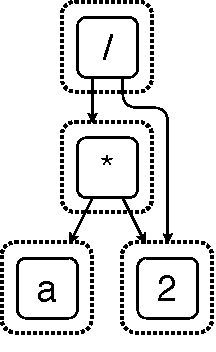
\includegraphics[height=30mm]{overview1.pdf}
%     \caption{Initial \egraph contains ${(a \times 2) / 2}$.}
%     \label{fig:egraph-rewrite1}
%   \end{subfigure}
%   \hfill
%   \begin{subfigure}[t]{0.23\linewidth}
%     \centering
%     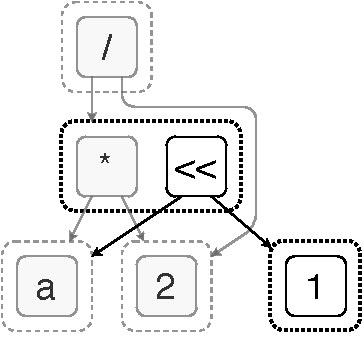
\includegraphics[height=30mm]{overview2.pdf}
%     \caption{
%       After applying rewrite ${x \times 2 \to x \ll 1}$.
%     }
%     \label{fig:egraph-rewrite2}
%   \end{subfigure}
%   \hfill
%   \begin{subfigure}[t]{0.23\linewidth}
%     \centering
%     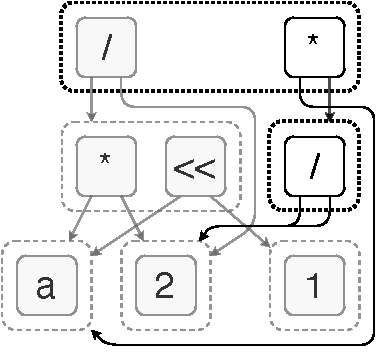
\includegraphics[height=30mm]{overview3.pdf}
%     \caption{
%       After applying rewrite ${(x \times y) / z \to x \times (y / z)}$.
%     }
%     \label{fig:egraph-rewrite3}
%   \end{subfigure}
%   \hfill
%   \begin{subfigure}[t]{0.24\linewidth}
%     \centering
%     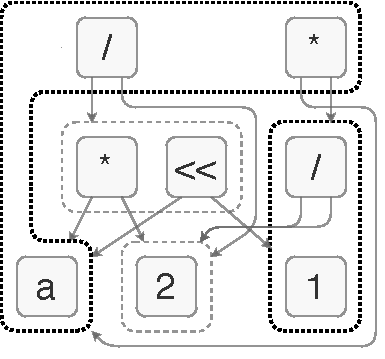
\includegraphics[height=30mm]{overview4.pdf}
%     \caption{
%       After applying rewrites ${x / x \to 1}$ and ${1 \times x \to x}$.
%     }
%     \label{fig:egraph-rewrite4}
%   \end{subfigure}
%   \caption{
%     An \egraph consists of \eclasses (dashed boxes) containing
%       equivalent \enodes (solid boxes).
%     Edges connect \enodes to their child \eclasses.
%     Additions and modifications are emphasized in black.
%     Applying rewrites to an \egraph adds new \enodes and edges,
%       but nothing is removed.
%     Expressions added by rewrites are merged with the matched \eclass.
%     In \autoref{fig:egraph-rewrite4}, the rewrites do not add any new nodes,
%       only merge \eclasses.
%     The resulting \egraph has a cycle,
%       representing infinitely many expressions:
%       $a$, $a \times 1$, $a \times 1 \times 1$, and so on.
%   }
%   \label{fig:egraph-rewrite}
% \end{figure}
\begin{figure}
  \begin{subfigure}[t]{0.175\linewidth}
    \centering
    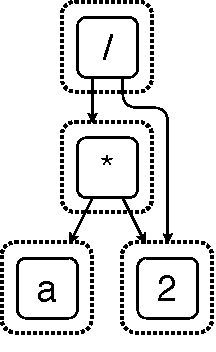
\includegraphics[height=30mm]{overview1.pdf}
    \caption{初始化包含\, ${(a \times 2) / 2}$ \,的\, \egraph}
    \label{fig:egraph-rewrite1}
  \end{subfigure}
  \hfill
  \begin{subfigure}[t]{0.23\linewidth}
    \centering
    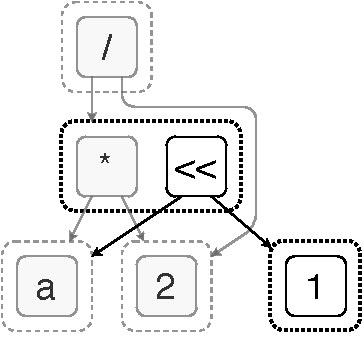
\includegraphics[height=30mm]{overview2.pdf}
    \caption{
      施加重写规则\, ${x \times 2 \to x \ll 1}$
    }
    \label{fig:egraph-rewrite2}
  \end{subfigure}
  \hfill
  \begin{subfigure}[t]{0.23\linewidth}
    \centering
    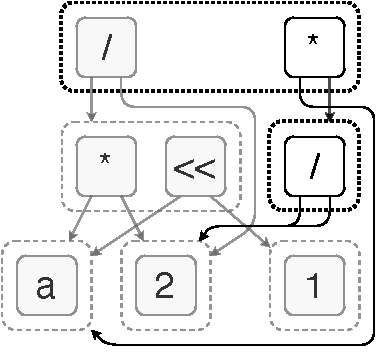
\includegraphics[height=30mm]{overview3.pdf}
    \caption{
      施加重写规则\, ${(x \times y) / z \to x \times (y / z)}$
    }
    \label{fig:egraph-rewrite3}
  \end{subfigure}
  \hfill
  \begin{subfigure}[t]{0.24\linewidth}
    \centering
    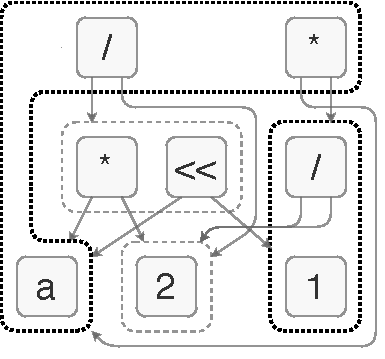
\includegraphics[height=30mm]{overview4.pdf}
    \caption{
      施加重写规则\, ${x / x \to 1}$ 和 ${1 \times x \to x}$
    }
    \label{fig:egraph-rewrite4}
  \end{subfigure}
  \caption{
    一张 \egraph 由包含等价的 \enodes(实心框)的 \eclasses (虚线框)组成。
    连接线连结 \enodes 到它们的 \eclasses 。
    加黑之处是增加和修改的部分。
    将重写应用于一个 \egraph 会增加新的 \enodes 和边线。但没有删除任何东西。
    通过改写增加的表达式会与匹配的 \eclass 合并。
    在 \autoref{fig:egraph-rewrite4} 中,改写不增加任何新节点,只是合并 \eclass。
      由此产生的 \egraph 有一个循环,代表无限多的表达式:
      $a$, $a \times 1$, $a \times 1 \times 1$, 以此类推。
  }
  \label{fig:egraph-rewrite}
\end{figure}


% \subsubsection{Interface and Rewriting}
\subsubsection{接口和重写}
\label{sec:interface}

% \Egraphs bear many similarities to the classic union-find data
%   structure that they employ internally,
%   and they inherit much of the terminology.
% \Egraphs provide two main low-level mutating operations:
\Egraphs 与经典的数据结构并查集有许多相似之处,它在内部采用了这种结构,继承了很多术语。
\Egraphs 提供了两个主要的低级变异操作:

% \begin{itemize}
%     \item \texttt{add} takes an \enode $n$ and:
%     \begin{itemize}
%         \item if $\texttt{lookup}(n) = a$, return $a$;
%         \item if $\texttt{lookup}(n) = \emptyset$,
%               then set $M[a] = \{ n \}$ and return the id $a$.
%     \end{itemize}
%     \item \texttt{merge} (sometimes called \texttt{assert} or \texttt{union})
%     takes two \eclass ids $a$ and $b$,
%     unions them in the union-find $U$,
%     and combines the \eclasses by setting both $M[a]$ and $M[b]$ to $M[a] \cup M[b]$.
% \end{itemize}
\begin{itemize}
    \item \texttt{add} 接受一个 \enode $n$ 进行:
    \begin{itemize}
        \item 如果 $\texttt{lookup}(n) = a$, 返回 $a$;
        \item 如果 $\texttt{lookup}(n) = \emptyset$,
              则设置 $M[a] = \{ n \}$ 并且返回 id $a$.
    \end{itemize}
    \item \texttt{merge} (有些时候称为 \texttt{assert} 或 \texttt{union})
    接受两个 \eclass id :$a$ 和 $b$,
    在并查集 $U$ 中合并它们, 
    然后通过设置 $M[a]$ 与 $M[b]$ 到 $M[a] \cup M[b]$ 拼合 \eclasses 。 % ?combines 拼合
\end{itemize}

% Both of these operations must take additional steps to maintain the congruence
%   invariant.
% Invariant maintenance is discussed in \autoref{sec:rebuilding}.
这两种操作都必须采取额外的步骤来维持同余的不变量。
不变量维护将在 \autoref{sec:rebuilding} 中讨论。

% \Egraphs also offers operations for querying the data structure.
\Egraphs 还提供了查询数据结构的操作:

% \begin{itemize}
%     \item \texttt{find} canonicalizes \eclass ids using the union-find $U$ as described in definition \ref{def:egraph}.
%     \item \texttt{ematch} performs the
%           \textit{e-matching}~\cite{simplify, ematching}
%           procedure for finding patterns in the \egraph.
%           \texttt{ematch} takes a pattern term $p$ with variable placeholders
%           and returns a list of tuples $(\sigma, c)$ where $\sigma$ is a substitution of
%           variables to \eclass ids such that $p[\sigma]$ is represented in \eclass $c$.
% \end{itemize}
\begin{itemize}
    \item \texttt{find} 规范化 \eclass id 使用在定义 \ref{def:egraph} 中描述的并查集 $U$。
    \item \texttt{find} 使用并查集 $U$ 来规范化 \eclass id,
    如定义 \ref{def:egraph} 中所述。
    \item \texttt{ematch} 执行在 \egraph 中查找模式的 
          \textit{e-matching}~\cite{simplify, ematching} 过程。 
          \texttt{ematch} 接受一个具有变量占位符的模式项 $p$ 并返回一个元组列表 $(\sigma, c)$,
          其中 $\sigma$ 是变量到 \eclass id 的替换,使得 $p[\sigma]$ 能在 \eclass $c$ 中表示。
            % ? 
\end{itemize}


% These can be composed to perform rewriting over the
%   \egraph.
% To apply a rewrite $\ell \to r$ to an \egraph,
%   \texttt{ematch}
%   finds tuples $(\sigma, c)$ where \eclass $c$ represents $\ell[\sigma]$.
% Then, for each tuple,
%   \mbox{\texttt{merge($c$, add($r[\sigma]$))}} adds $r[\sigma]$ to the \egraph
%   and unifies it with the matching \eclass c.
这些可以组合起来对 \egraph 执行重写。
要在 \egraph 上应用重写 $\ell \to r$ ,
  \texttt{ematch} 会找到元组 $(\sigma, c)$ ,其中 \eclass $c$ 表示 $\ell[\sigma]$ 。
然后,对于每个元组,
  \mbox{\texttt{merge($c$, add($r[\sigma]$))}} 将 $r[\sigma]$ 添加到 \egraph 中,
  并使其与匹配的 \eclass c 统一。


% \autoref{fig:egraph-rewrite} shows an \egraph undergoing a series of rewrites.
% Note how the process is only additive; the initial term $(a \times 2) / 2$ is
%   still represented in the \egraph.
% Rewriting in an \egraph can also saturate, meaning the \egraph has
%   learned every possible equivalence derivable from the given rewrites.
% % This not only solves the phase ordering problem, but also handles rules like
% %   commutativity that can be troublesome to a conventional rewrite system.
% If the user tried to apply $x \times y \to y \times x$ to an \egraph twice,
%   the second time would add no additional \enodes and perform no new merges;
%   the \egraph can detect this and stop applying that rule.
\autoref{fig:egraph-rewrite} 展示了一个经历了一系列重写的 \egraph。
注意这个过程只是增加性的;初始项 $(a \times 2) / 2$ 仍然在 \egraph 中表示。
在 \egraph 中重写也可以饱和,这意味着 \egraph 已经学会了给定重写可以推出的所有等价关系。
% 这不仅解决了阶段顺序问题,还能处理像交换律这样的规则,这对于传统重写系统来说可能有困难。
如果用户试图将 $x \times y \to y \times x$ 应用于 \egraph 两次,
  第二次将不会添加额外的 \enodes 并不会进行新的合并;\egraph 可以检测到这一点并停止应用该规则。

\subsection{等式饱和(Equality Saturation)}
\label{sec:eqsat}

% Term rewriting~\cite{nachum-rewrites} is a time-tested approach
%   for equational reasoning in
%   program optimization~\cite{eqsat, denali},
%   theorem proving~\cite{simplify, z3},
%   and program transformation~\cite{graphs}.
% In this setting, a tool repeatedly chooses one of a set of axiomatic rewrites,
%   searches for matches of the left-hand pattern in the given
%   expression, and replaces matching instances with the substituted
%   right-hand side.
项重写 ~\cite{nachum-rewrites} 是一种久经考验的方法,
  它针对于程序综合~\cite{eqsat, denali}、
  定理证明~\cite{simplify, z3}、
  程序转换~\cite{graphs},
  中的等式推理
在这种情况下,一个工具重复选择一组公理改写中的一个。
  在给定的表达式中搜索与左式相匹配的表达式,并将匹配的实例替换为被替换的右式。

% Term rewriting is typically destructive and ``forgets'' the matched
%   left-hand side.
% Consider applying a simple strength reduction rewrite:
%   ${ (a \times 2) / 2 \to (a \ll 1) / 2 }$.
% The new term carries no
%   information about the initial term.
% Applying strength reduction at this point prevents us from canceling out $2/2$.
% In the compilers community, this classically tricky question of when to apply
%   which rewrite is called the \textit{phase ordering} problem.
项重写通常是破坏性的并且“忘记”了匹配的左式。
考虑应用一个简单的降低计算量(strength reduction)重写:
  ${ (a \times 2) / 2 \to (a \ll 1) / 2 }$。
新项不带有初始项的信息。在此之前应用降低计算量重写阻止我们消除 $2/2$。
在编译器社群中,这个关于何时应用哪个重写的问题被称为\textit{编译优化选择(phase ordering)}问题。


% One solution to the phase ordering problem would simply apply all
%   rewrites simultaneously, keeping track of every expression seen.
% This eliminates the problem of choosing the right rule, but
%   a naive implementation would require space exponential in the number
%   of given rewrites.
% \textit{Equality saturation}~\cite{eqsat, eqsat-llvm} is a technique to do this
%   rewriting efficiently using an \egraph.
解决编译优化选择问题的一种方法是同时应用所有重写,并跟踪每个表达式。
这消除了选择正确规则的问题,但是简单实现需要给定重写数量的指数级空间。
\textit{等式饱和(equality saturation)}~\cite{eqsat, eqsat-llvm} 是一种使用 \egraph 有效地进行此重写的技术。

% \begin{figure}
%   \begin{minipage}{0.48\linewidth}
%     \centering
%     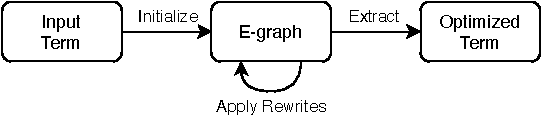
\includegraphics[width=0.9\linewidth]{eqsat}
%   \end{minipage}
%   \hfill
%   \begin{minipage}{0.46\linewidth}
%   \begin{lstlisting}[language=Python, gobble=4, numbers=left, basicstyle=\scriptsize\ttfamily]
%     def equality_saturation(expr, rewrites):
%       egraph = initial_egraph(expr)

%       while not egraph.is_saturated_or_timeout():

%         for rw in rewrites:
%           for (subst, eclass) in egraph.ematch(rw.lhs):
%             eclass2 = egraph.add(rw.rhs.subst(subst))
%             egraph.merge(eclass, eclass2)

%       return egraph.extract_best()
%   \end{lstlisting}
%   \end{minipage}
%   \caption{
%     Box diagram and pseudocode for equality saturation.
%     Traditionally, equality saturation maintains the \egraph data structure
%       invariants throughout the algorithm.
%   }
%   \label{fig:eq-sat-bg}
% \end{figure}
\begin{figure}
  \begin{minipage}{0.48\linewidth}
    \centering
    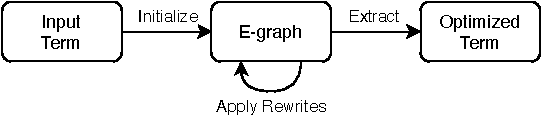
\includegraphics[width=0.9\linewidth]{eqsat}
  \end{minipage}
  \hfill
  \begin{minipage}{0.46\linewidth}
  \begin{lstlisting}[language=Python, gobble=4, numbers=left, basicstyle=\scriptsize\ttfamily]
    def equality_saturation(expr, rewrites):
      egraph = initial_egraph(expr)

      while not egraph.is_saturated_or_timeout():

        for rw in rewrites:
          for (subst, eclass) in egraph.ematch(rw.lhs):
            eclass2 = egraph.add(rw.rhs.subst(subst))
            egraph.merge(eclass, eclass2)

      return egraph.extract_best()
  \end{lstlisting}
  \end{minipage}
  \caption{
    等式饱和 的框图和伪代码。
    传统上,等式饱和 在整个算法中保持 \egraph 数据结构不变量。
  }
  \label{fig:eq-sat-bg}
\end{figure}


% \autoref{fig:eq-sat-bg} shows the equality saturation workflow.
% First, an initial \egraph is created from the input term.
% The core of the algorithm runs a set of rewrite rules until the \egraph is
%   saturated (or a timeout is reached).
% Finally, a procedure called \textit{extraction} selects the optimal represented
%   term according to some cost function.
% For simple cost functions, a bottom-up, greedy traversal of the \egraph suffices
%   to find the best term.
% Other extraction procedures have been explored for more complex cost
%   functions~\cite{spores, wu_siga19}.
\autoref{fig:eq-sat-bg} 展示了 等式饱和 工作流程。
首先,从输入的项创建初始 \egraph。
算法的核心运行一组重写规则,直到 \egraph 饱和或超时。
最后,称为 \textit{extraction(提取)} 的程序根据某些成本函数选择最优表示的项。
对于简单的成本函数,自底向上贪心遍历 \egraph 足以找到最佳术语。
其他提取程序已经探索了更复杂的成本函数~\cite{spores, wu_siga19}。

% Equality saturation eliminates the tedious and often error-prone
%   task of choosing when to apply which rewrites,
% %Equality saturation turns a correctness problem into a performance problem,
%   promising an appealingly simple workflow: state the
%   relevant rewrites for the language, create an initial \egraph from a given
%   expression, fire the rules until saturation,
%   and finally extract the cheapest equivalent expression.
% Unfortunately, the technique remains ad hoc; prospective equality saturation
%   users must implement their own \egraphs customized to their language, avoid
%   performance pitfalls, and hack in the ability to do interpreted reasoning
%   that is not supported by purely syntactic rewrites.
% \egg aims to address each aspect of these difficulties.
等式饱和 消除了选择何时应用哪些重写的繁琐而容易出错的任务,
提供了一种简单易用的工作流程:确定语言相关重写,从给定表达式创建初始 \egraph ,运行规则直到饱和,
  最后提取最优的等价表达式。
不幸的是,这种技术仍然是特别定制的,
  等式饱和 用户必须自己实现专门针对语言的 \egraph,
  避免性能问题,并通过骇入(hack in)的方法实现纯语法重写无法支持的解释性推理。
\egg 旨在解决这些困难。

% \subsection{Equality Saturation and Theorem Proving}
\subsection{等式饱和 和 定理证明}

% An equality saturation engine and a theorem prover each have capabilities that
%   would be impractical to replicate in the other.
% Automated theorem provers like satisfiability modulo theory (SMT) solvers are
%   general tools that, in addition to supporting satisfiability queries,
%   incorporate sophisticated, domain-specific solvers to allow interpreted
%   reasoning within the supported theories.
% On the other hand, equality saturation is specialized for optimization, and its
%   extraction procedure directly produces an optimal term with respect to a given
%   cost function.
% % To replicate extraction with an SMT solver, one would have to resort to a more
% %   expensive enumerative approach.
等式饱和 引擎和定理验证器都有一些能力在对方身上复制是不切实际的。
像可满足模理论(SMT)求解器这样的自动化定理证明器是通用工具,
  除了支持可满足性查询外,还整合了专业的,领域特定的求解器,允许在支持的理论内进行解释性推理。
另一方面,等式饱和 是专门用于优化的,其提取过程直接产生关于给定成本函数的最优的项。

% \James{What enumerative approach? How do you know that one would "have to" resort to it?}

% While SMT solvers are indeed the more general tool,
%   equality saturation is not superseded by SMT;
%   the specialized approach can be much faster when the full generality of SMT is
%   not needed.
% To demonstrate this, we replicated a portion of the recent TASO paper~\cite{taso},
%   which optimizes deep learning models.
% As part of the work, they must verify a set of synthesized equalities with
%   respect to a trusted set of universally quantified axioms.
% TASO uses Z3~\cite{z3} to perform the
%   verification even though most of Z3's features
%   (disjunctions, backtracking, theories, etc.)
%   were not required.
% An equality saturation engine can also be used for verifying these equalities
%   by adding the left and right sides of
%   each equality to an \egraph,
%   running the axioms as rewrites,
%   and then checking if both sides end up in the same \eclass.
% Z3 takes 24.65 seconds to perform the verification;
%   \egg performs the same task in 1.56 seconds ($15\times$ faster),
%   or only 0.52 seconds ($47\times$ faster) when using
%   \egg's batched evaluation (\autoref{sec:egg-batched}).
尽管SMT求解器确实是更通用的工具,但 等式饱和 并不被 SMT 取代;
  当不需要 SMT 的完全通用性时,特异化的方法可能更快。
为了证明这一点,我们复制了最近 TASO 论文的一部分~\cite{taso},它优化了深度学习模型。
作为工作的一部分,他们必须验证一组合成等式,它们需要遵守一组具有普遍性的公理。 %?respect to 
TASO 使用 Z3~\cite{z3} 执行验证,即使大部分Z3的功能(或运算、回溯、理论等)都不需要使用。
等式饱和 也可以用于验证这些等式,
  将每个等式的左右两侧添加到 \egraph 中,将公理作为重写规则运行,
  然后检查两侧是否最终在同一个 \eclass 中。
Z3 花费 24.65 秒进行验证;\egg 在1.56秒(快 $15\times$)中完成相同任务,
  或在使用 \egg 的批量评估(\autoref{sec:egg-batched})时只需要 0.52 秒(快 $47\times$ )。
  
% --------------------

% \James{
  % The experimental/perf numbers in the last par of 2.4 feel out of place. Not sure how to fix...
% }

% However, their abilities overlap on a specific kind of theorem proving:
%   given a list of axioms in the form of universal quantified equalities,
%   prove two (or more) terms equal.
% Some SMT solvers support these kinds of queries, albeit in a limited fashion
%   since they are undecidable.
% \footnotetext{
%   Since these queries are undecidable, both SMT solvers and equality
%   saturation engines can either prove the inputs equal or fail to; they cannot
%   prove them unequal.
% }



%%% Local Variables:
%%% TeX-master: "egg"
%%% End:

\section{重建: \Egraph 不变量维护的全新视角}
% \section{Rebuilding: A New Take on \Egraph Invariant Maintenance}
\label{sec:rebuild}
\label{sec:rebuilding}

% Rebuilding is a new, general perspective on \egraph invariant maintenance.
% Traditionally~\cite{nelson, simplify},
%   \egraphs maintain their data structure invariants
%   after each operation.
% We separate this invariant restoration into a procedure called \textit{rebuilding}.
% This separation allows the client to
%   choose when to enforce the \egraph invariants.
% Performing a rebuild immediately after every operation replicates the
%   traditional approach to invariant maintenance.
% In contrast, rebuilding less frequently can amortize the cost of invariant
%   maintenance, significantly improving performance.
传统上~\cite{nelson, simplify},\egraphs 在每次操作后保持数据结构不变式。
我们将这种不变式恢复分为称为 \textit{rebuilding(重建)} 的过程。
这种分离允许客户端选择何时执行 \egraph 不变式。
立即在每次操作后执行重建就复制了传统的不变式维护方法,
相比之下,较少的重建可以摊销不变式维护成本,显著提高性能。

% In this section, we first describe how e-graphs have
%   traditionally maintained invariants (\autoref{sec:upward}).
% We then describe the rebuilding framework and how it captures a spectrum of
%   invariant maintenance approaches, including the traditional one
%   (\autoref{sec:rebuilding-detail}).
% Using this flexibility, we then give a modified algorithm for equality
%   saturation that enforces the \egraph invariants at only select points
%   (\autoref{sec:rebuilding-eqsat}).
% We finally demonstrate that this new approach offers an asymptotic speedup over
%   traditional equality saturation (\autoref{sec:rebuild-eval}).
在本节中,我们首先描述了 e-graphs 如何传统地维护不变量(\autoref{sec:upward})。
然后,我们描述了重构框架以及它如何捕获一系列维护不变量的方法,
  包括传统方法(\autoref{sec:rebuilding-detail})。
利用这种灵活性,我们然后给出了一种修改的算法,用于 等式饱和 ,
  它只在特定点强制执行 \egraph 不变量(\autoref{sec:rebuilding-eqsat})。  %?enforces the \egraph invariants
最后,我们证明这种新方法比传统的等价饱和提供了渐进加速 % ?asymptotic speedup
  (\autoref{sec:rebuild-eval})。



% 原文注释 begin
% Among \egg's optimizations (\autoref{sec:egg-efficient}),
%   strategically delayed rebuilding is perhaps the most important.
% \egg employed a m
% Delayed rebuilding amortizes the cost of invariant maintenance, significantly reducing work

% Rebuilding is a novel technique that lies at the heart of \egg's
%   modified equality saturation algorithm.
% This crucial technique allows equality saturation to specialize the \egraph to
%   its workload, yielding substantial performance improvements.
%   %from both an algorithmic and implementation
%   %perspective.

% Rebuilding gives the user (or algorithm) choice on when to restore the \egraph
%   invariants, which can have a large impact on performance .

% The key insight is that maintaining the \egraph invariants is expensive, and

% \autoref{fig:eq-sat-code} shows both the traditional and \egg's modified
%   equality saturation loop.
% The key distinction is \textit{when} the \egraph invariants of deduplication and
%   congruence are maintained.
% In traditional \egraphs, like with many data structures, invariants always
%   hold.
% In contrast, mutating an \egg \egraph may violate invariants, causing equalities
%   to be not ``seen'' when searching for patterns.
% \egg lets the user (or the algorithm) choose when to restore the invariants by
%   calling the \texttt{rebuild} method.
% Rebuilding leads to a lower amortized cost of maintaining the \egraph invariants.
% 原文注释 end

% \subsection{Upward Merging}
\subsection{向上合并}
\label{sec:upward}

% Both mutating operations on the \egraph
%   (\texttt{add} and \texttt{merge}, \autoref{sec:interface})
%   can break the \egraph invariants if not done carefully.
% \Egraphs have traditionally used \textit{hashconsing} and
%   \textit{upward merging} to maintain the congruence invariant.
如果不仔细操作,对 \egraph 进行的变异操作 (\texttt{add} 和 \texttt{merge},\autoref{sec:interface})
  可能会破坏 \egraph 不变性。
\Egraphs 传统上使用 \textit{哈希康化(hashconsing)} 和  % ?hashconsing
  \textit{向上合并(upward merging)} 来维护同余不变性。


% The \texttt{add} operation relies on the hashcons invariant
%   (Definition \ref{def:hash-inv})
%   to quickly check whether the \enode $n$ to be added---or one congruent to it---is
%   already present.
% Without this check, \texttt{add} would create a new \eclass with $n$ in it
%   even if some $n' \cong n$ was already in the \egraph,
%   violating the congruence invariant.
\texttt{add} 操作依赖于哈希康不变性 (hashcons invariant,定义 \ref{def:hash-inv}) 来
  快速检查要添加的 \enode $n$ 或与其同余的节点是否已经存在。
如果没有这个检查,\texttt{add} 将创建一个新的 \eclass,
  其中包含 $n$,即使某些 $n' \cong n$ 已经在 \egraph 中,这将违反同余不变性。


% The \texttt{merge} operation \eclasses can violate both \egraph invariants.
% If $f(a, b)$ and $f(a, c)$ reside in two different \eclasses $x$ and $y$,
%   merging $b$ and $c$ should also merge $x$ and $y$ to maintain the congruence invariant.
% This can propagate further, requiring additional merges.
\texttt{merge} 操作可能会违反 \egraph 的两个不变性。
如果 $f(a, b)$ 和 $f(a, c)$ 分别位于两个不同的 \eclasses $x$ 和 $y$ 中,
  合并 $b$ 和 $c$ 也应该合并 $x$ 和 $y$ 以维护同余不变性。
这可能会进一步传播,需要额外的合并。

%  % merging $x$ and $y$ could cause two other
%  %  \enodes to become congruent and require merging their \eclasses.

% \Egraphs maintain a \textit{parent list} for each \eclass
%   to maintain congruence.
% The parent list for \eclass $c$ holds all \enodes that have $c$ as a child.
% When merging two \eclasses, \egraphs inspect these parent lists to find parents
%   that are now congruent, recursively ``upward merging'' them if necessary.
\Egraphs 为每个 \eclass 维护一个 \textit{父列表(parent list)} 以维持同余。
\eclass $c$ 的父列表包含所有将 $c$ 作为子节点的 \enodes。
合并两个 \eclasses 时,\egraphs 检查这些父节点列表,找到现在同余的父节点,
  如果需要就递归进行 ``向上合并''。


% The \texttt{merge} routine must also perform bookkeeping to preserve the
%   hashcons invariant.
% In particular, merging two \eclasses may change how parent \enodes of those
%   \eclasses are canonicalized.
% The \texttt{merge} operation must therefore
%   remove, re-canonicalize, and replace those \enodes in the
%   hashcons.
% In existing \egraph implementations~\cite{herbie} used for equality saturation,
%   maintaining the invariants while merging can take the vast majority of
%   run time.
\texttt{merge} 程序还必须执行记录(bookkeeping)来保持哈希康不变性。
特别地,合并两个 \eclasses 可能会改变这些 \eclasses 的父 \enodes 如何规范化。
  因此 \texttt{merge} 操作必须在哈希康中删除、重规范化并替换这些 \enodes。 % ?
在用于 等式饱和 的现有 \egraph 实现 ~\cite{herbie} 中,
  在合并时维护不变性可能占用绝大部分运行时间。

% \subsection{Rebuilding in Detail}
\subsection{重建细节}
\label{sec:rebuilding-detail}


\begin{figure}
  \begin{minipage}[t]{0.47\linewidth}
    \begin{lstlisting}[gobble=4, numbers=left, basicstyle=\scriptsize\ttfamily, escapechar=|]
    def add(enode):
      enode = self.canonicalize(enode)
      if enode in self.hashcons:
        return self.hashcons[enode]
      else:
        eclass_id = self.new_singleton_eclass(enode)
        for child in enode.children:
          child.parents.add(enode, eclass_id)
        self.hashcons[enode] = eclass_id
        return eclass_id

    def merge(id1, id2)
      if self.find(id1) == self.find(id2):
        return self.find(id1)
      new_id = self.union_find.union(id1, id2)
      # 传统的 egraph 合并可以通过
      # 在将 eclass 添加到 worklist 之后
      # 立即调用重建来模拟。
      self.worklist.add(new_id) |\label{line:worklist-add}|
      return new_id

    def canonicalize(enode) |\label{line:canon}|
      new_ch = [self.find(e) for e in enode.children]
      return mk_enode(enode.op, new_ch)

    def find(eclass_id):
      return self.union_find.find(eclass_id)
    \end{lstlisting}
  \end{minipage}
  \hfill
  \begin{minipage}[t]{0.47\linewidth}
    \begin{lstlisting}[gobble=4, numbers=left, firstnumber=27, basicstyle=\scriptsize\ttfamily]
    def rebuild():
      while self.worklist.len() > 0:
        # 将 worklist 清空到一个局部变量中
        todo = take(self.worklist)
        # 对 eclass refs 进行规范化和去重,
        # 以节省 repair 调用的次数。
        todo = { self.find(eclass) for eclass in todo }
        for eclass in todo:
          self.repair(eclass)

    def repair(eclass):
      # 更新 hashcons,
      # 使其总是指向规范的 enodes 到规范的 eclasses。
      for (p_node, p_eclass) in eclass.parents:
        self.hashcons.remove(p_node)
        p_node = self.canonicalize(p_node)
        self.hashcons[p_node] = self.find(p_eclass)

      # 去重父节点,
      # 注意等价的父节点会被合并并放在 worklist 中。
      new_parents = {}
      for (p_node, p_eclass) in eclass.parents:
        p_node = self.canonicalize(p_node)
        if p_node in new_parents:
          self.merge(p_eclass, new_parents[p_node])
        new_parents[p_node] = self.find(p_eclass)
      eclass.parents = new_parents
    \end{lstlisting}
  \end{minipage}
  \caption{
    % Pseudocode for the \texttt{add}, \texttt{merge}, \texttt{rebuild}, and
    % supporting methods.
    % In each method, \texttt{self} refers to the \egraph being modified.
     \texttt{add}, \texttt{merge}, \texttt{rebuild} 和一些支持的方法的伪代码。
    在以上每个方法中, \texttt{self} 指的是正被修改的 \egraph 。
    % 【代码注释翻译】 翻译时注意保留原本的行数!
    %       # traditional egraph merge can be
    %   # emulated by calling rebuild right after
    %   # adding the eclass to the worklist
    % 1. 传统的 egraph 合并可以通过在将 eclass 添加到 worklist 之后立即调用重建来模拟。
    %     # empty the worklist into a local variable
    % 2. 将 worklist 清空到一个局部变量中
    %         # canonicalize and deduplicate the eclass refs
    %     # to save calls to repair
    % 3. 对 eclass refs 进行规范化和去重,以节省 repair 调用的次数。
    %       # update the hashcons so it always points
    %   # canonical enodes to canonical eclasses
    % 4. 更新 hashcons,使其总是指向规范的 enodes 到规范的 eclasses。
    %       # deduplicate the parents, noting that equal
    %   # parents get merged and put on the worklist
    % 5. 去重父节点,注意等价的父节点会被合并并放在 worklist 中。
  }
  \label{fig:rebuild-code}
\end{figure}

% Traditionally, invariant restoration is part of the
%   \texttt{merge} operation itself.
% Rebuilding separates these concerns,
%   reducing \texttt{merge}'s obligations
%   and allowing for amortized invariant maintenance.
% In the rebuilding paradigm,
%   \texttt{merge} maintains a \textit{worklist} of \eclass ids that need to
%   be ``upward merged'', i.e., \eclasses whose parents are possibly congruent but
%   not yet in the same \eclass.
% The \texttt{rebuild} operation processes this worklist, restoring the invariants
%   of deduplication and congruence.
% Rebuilding is similar to other approaches in how it restores congruence
%   (see \nameref{sec:related} for comparison to \citet{downey-cse});
%   but it uniquely allows the client to choose when to restore invariants in the
%   context of a larger algorithm like equality saturation.
传统上,不变量恢复是 \texttt{merge} 操作本身的一部分。
重建将这些关注点分开,减少 \texttt{merge} 的责任并允许摊销不变量维护的工作。
在重建范式中,\texttt{merge} 保持一个 \textit{工作列表(worklist)},
  其中包含需要 "向上合并" 的 \eclass id,
  即父节点可能同余但尚未在同一 \eclass 中的 \eclasses。
\texttt{rebuild} 操作处理这个工作列表,
  恢复去重(deduplication)和同余(congruence)的不变量。
重建在如何恢复同余中类似于其他方法,
  (见 \nameref{sec:related} 与 \citet{downey-cse} 的比较);
  但特别的是它允许客户在更大规模的算法(如 等式饱和)上选择何时恢复不变量。

% \autoref{fig:rebuild-code} shows pseudocode for the main \egraph operations and
%   rebuilding.
% Note that \texttt{add} and \texttt{canonicalize} are given for completeness, but
%   they are unchanged from the traditional \egraph implementation.
% The \texttt{merge} operation is similar, but it only adds the new \eclass to the
%   worklist instead of immediately starting upward merging.
% Adding a call to \texttt{rebuild} right after the addition to
%   the worklist (\autoref{fig:rebuild-code} line \ref{line:worklist-add})
%   would yield the traditional behavior of restoring the invariants immediately.
\autoref{fig:rebuild-code} 展示了主 \egraph 操作和重建的伪代码。
请注意,为了完整性起见,给出了 \texttt{add} 和 \texttt{canonicalize},
  但它们与传统的 \egraph 实现相同。
\texttt{merge} 操作类似,但它只将新的 \eclass 添加到工作列表中,而不是立即开始向上合并。
在工作列表添加后立即调用 \texttt{rebuild} 
  (\autoref{fig:rebuild-code} 第 \ref{line:worklist-add} 行)
  将产生传统行为——立即恢复不变性。


% The \texttt{rebuild} method essentially calls \texttt{repair} on the \eclasses
%   from the worklist until the worklist is empty.
% Instead of directly manipulating the worklist, \egg's \texttt{rebuild} method
%   first moves it into a local variable and deduplicates \eclasses
%   up to equivalence.
% Processing the worklist may \texttt{merge} \eclasses,
%   so breaking the worklist into chunks ensures that \eclass ids made
%   equivalent in the previous chunk are deduplicated in the subsequent chunk.
\texttt{rebuild} 方法实质上是在工作列表上的 \eclasses 上调用 \texttt{repair},
  直到工作列表为空。
与直接操作工作列表不同,\egg 的 \texttt{rebuild} 方法首先将其移动到局部变量中,
  并对 \eclasses 进行去重直到等价(equivalence)。
处理工作列表可能会 \texttt{merge} \eclasses,
  所以将工作列表分成几块,以确保在前一块中被等价的 \eclass id 在随后的几块中被去重。

% 本段翻译未仔细校对
% The actual work of \texttt{rebuild} occurs in the \texttt{repair} method.
% \texttt{repair} examines an \eclass $c$ and first canonicalizes \enodes in the
%   hashcons that have $c$ as a child.
% Then it performs what is essentially one ``layer'' of upward
%   merging:
% if any of the parent \enodes have become congruent, then their
%   \eclasses are merged and the result is added to the worklist.
\texttt{rebuild} 的实际工作发生在 \texttt{repair} 方法中。
\texttt{repair} 检查 \eclass $c$,
  首先在 hashcons 中对具有 $c$ 作为子项的 \enodes 进行规范化。
然后,它执行的基本上是一个“层”的向上的合并。
如果父节点中有任何一个已经变得等价,则它们的 \eclasses 被合并,结果被添加到工作列表中。


% 本段翻译未仔细校对
% Deduplicating the worklist, and thus reducing calls to \texttt{repair},
%   is at the heart of why deferring rebuilding improves
%   performance.
% Intuitively, the upward merging process of rebuilding traces out a ``path'' of
%   congruence through the \egraph.
% When rebuilding happens immediately after \texttt{merge}
%   (and therefore frequently), these paths can substantially overlap.
% By deferring rebuilding, the chunk-and-deduplicate approach can coalesce the
% overlapping parts of these paths, saving what would have been redundant work.
% In our modified equality saturation algorithm (\autoref{sec:rebuilding-eqsat}),
%   deferred rebuilding is responsible for a significant, asymptotic speedup
%   (\autoref{sec:rebuild-eval}).
工作列表的去重,从而减少对 \texttt{repair} 的调用,是延迟重建改善性能的核心。
直观地说,重建的上升合并过程追踪 \egraph 中的同余``路径''。
当重建立即发生在 \texttt{merge} 之后(因此经常发生)时,这些路径可能会大量重叠。
通过延迟重建,块和去重方法可以合并这些路径的重叠部分,节省了原本冗余的工作。
在我们修改的等价饱和算法中(\autoref{sec:rebuilding-eqsat}),
  延迟重建对性能有着显著的改善(\autoref{sec:rebuild-eval})。

% \subsubsection{Examples of Rebuilding}
\subsubsection{重建的例子}

% 本段翻译未仔细校对
% Deferred rebuilding speeds up congruence maintenance by amortizing the work of
%   maintaining the hashcons invariant.
% Consider the following terms in an \egraph:
%   $f_{1}(x), ..., f_{n}(x),\, y_{1}, ..., y_{n}$.
% Let the workload be $\texttt{merge}(x, y_{1}), ..., \texttt{merge}(x, y_{n})$.
% Each merge may change the canonical representation of the $f_{i}(x)$s,
%   so the traditional invariant maintenance strategy
%   could require $O(n^{2})$ hashcons updates.
% With deferred rebuilding the \texttt{merges} happen before
%   the hashcons invariant is restored,
%   requiring no more than $O(n)$ hashcons updates.
延迟重建通过摊销维护 hashcon 不变量的工作来加速同余的维护 % 直接中文开头有bug
考虑以下 \egraph 中的 term:
  $f_{1}(x), ..., f_{n}(x),, y_{1}, ..., y_{n}$。
工作量为 $\texttt{merge}(x, y_{1}), ..., \texttt{merge}(x, y_{n})$。
每次合并可能会更改 $f_{i}(x)$ 的规范表示,
  因此传统的不变性维护策略可能需要 $O(n^{2})$ 的 hashcons 更新。
通过延迟重建,\texttt{merge} 在恢复 hashcons 不变性之前发生,
  最多只需要 $O(n)$ 个 hashcons 更新。


% 本段翻译未仔细校对
% Deferred rebuilding can also reduce the number of calls to \texttt{repair}.
% Consider the following $w$ terms in an \egraph,
%   each nested under $d$ function symbols:
%   $$f_1 (f_2(\ldots f_d(x_1))), \quad\ldots,\quad f_1(f_2(\ldots f_d(x_w)))$$
% Note that $w$ corresponds the width of this group of terms, and $d$ to the depth.
% Let the workload be $w-1$ merges that merge all the $x$s together:
%   for $i \in [2, w], \texttt{merge}(x_{1}, x_{i})$.
延迟重建还可以减少调用 \texttt{repair} 的次数。
考虑以下 \egraph 中的 $w$ 个 term,每个都嵌套在 $d$ 函数符号之下:
  $$f_1 (f_2(\ldots f_d(x_1))), \quad\ldots,\quad f_1(f_2(\ldots f_d(x_w)))$$
请注意,$w$ 对应于这组 term 的宽度,$d$ 对应深度。
工作量为 $w-1$ 次合并,将所有 $x$ 合并在一起:
  for $i \in [2, w], \texttt{merge}(x_{1}, x_{i})$。

% 本段翻译未仔细校对
% In the traditional upward merging paradigm
%   where \texttt{rebuild} is called after every \texttt{merge},
%   each $\texttt{merge}(x_i, x_j)$ will require $O(d)$ calls to \texttt{repair}
%   to maintain congruence, one for each layer of $f_{i}$s.
% Over the whole workload, this requires $O(wd)$ calls to \texttt{repair}.
在传统的向上合并范式中,每次调用 \texttt{merge} 后都会调用 \texttt{rebuild},
  每次 $\texttt{merge}(x_i, x_j)$ 都需要 $O(d)$ 次调用 \texttt{repair} 来维护同余,
  每层 $f_{i}$ 都需要一次。
在整个工作量中,这需要 $O(wd)$ 次调用 \texttt{repair}。


% 本段翻译未仔细校对
% With deferred rebuilding, however, the $w-1$ merges can all take place before
%   congruence must be restored.
% Suppose the $x$s are all merged into an \eclass $c_{x}$
% When \texttt{rebuild} finally is called,
%   the only element in the deduplicated worklist is $c_{x}$.
% Calling \texttt{repair} on $c_{x}$ will merge the \eclasses of the $f_{d}$
%   \enodes into an \eclass $c_{f_{d}}$,
%   adding the \eclasses that contained those \enodes back to the worklist.
% When the worklist is again deduplicated,
%   $c_{f_{d}}$ will be the only element,
%   and the process repeats.
% Thus, the whole workload only incurs $O(d)$ calls to \texttt{repair},
%   eliminating the factor corresponding to the width of this group of terms.
% \autoref{fig:repair-plot} shows that the number calls to \texttt{repair} is
%   correlated with time spent doing congruence maintenance.
然而,使用延迟重建时,可以在恢复同余之前进行 $w-1$ 次合并。
假设 $x$ 全部合并到 \eclass $c_{x}$ 中。
在最后调用 \texttt{rebuild} 时,去重工作列表中唯一的元素是 $c_{x}$。
调用 $c_{x}$ 上的 \texttt{repair} 将 $f_{d}$ 的 \eclasses 合并到 \eclass $c_{f_{d}}$ 中,
  并将包含这些 \enodes 的 \eclasses 添加回工作列表。
当工作列表再次去重时,$c_{f_{d}}$ 将是唯一的元素,过程将重复。
因此,整个工作量只会产生 $O(d)$ 次调用 \texttt{repair},
  消除了与这组术语宽度相关的因素。
\autoref{fig:repair-plot} 表明调用 \texttt{repair} 的次数与进行同余维护的时间相关。


% \subsubsection{Proof of Congruence}
\subsubsection{同余性的证明}

% 本段翻译未仔细校对
% Intuitively, rebuilding is a delay of the upward merging process, allowing
%   the user to choose when to restore the \egraph invariants.
% They are substantially similar in structure, with a critical a difference in when
%   the code is run.
% Below we offer a proof demonstrating that rebuilding restores the
% \egraph congruence invariant.
直观上,重建是对向上合并过程的延迟,允许用户选择何时恢复 \egraph 不变性。
它们在结构上实质上相似,关键的区别在于代码何时运行。
下面我们提供了一个证明,证明重建恢复了 \egraph 同余不变性。

\begin{theorem}
  % Rebuilding restores congruence and terminates.
  重建恢复了同余并终止。(Rebuilding restores congruence and terminates.) % ?
\end{theorem}

\begin{proof}
%   本段翻译未仔细校对
%   Since rebuilding only merges congruent nodes,
%     the congruence closure $\cong^{*}$ is fixed even though $\equivnode$ changes.
%   When $(\equivnode) = (\cong^*)$, congruence is restored.
%   Note that both $\equivnode$ and $\cong^*$ are finite.
%   We therefore show that rebuilding causes $\equivnode$ to approach $\cong^*$.
%   We define the set of incongruent \enode pairs as $I = (\cong^*) \setminus (\equivnode)$;
%   in other words,
%     $(n_{1}, n_{2}) \in I$ if $n_{1} \cong^{*} n_{2}$
%      but $n_{1} \not\equivnode n_{2}$.
% %    have the same function symbol
% %    and equivalent children, but are not yet in the same \eclass.
  因为重建只合并等价节点,即使 $\equivnode$ 改变,同余闭包 $\cong^{*}$ 也是固定的。
  当 $(\equivnode) = (\cong^*)$ 时,同余被恢复。
  注意 $\equivnode$ 和 $\cong^*$ 都是有限的。
  因此,我们证明重建导致 $\equivnode$ 接近 $\cong^*$。
  我们定义不同余 \enode 对的集合 $I = (\cong^*) \setminus (\equivnode)$;
  换句话说,
    当 $(n_{1}, n_{2}) \in I$ 时 
    $n_{1} \cong^{*} n_{2}$ 
    但 $n_{1} \not\equivnode n_{2}$。

%   本段翻译未仔细校对
  % Due to the additive nature of equality saturation, $\equivnode$ only increases
  %   and therefore $I$ is non-increasing.
  % However, a call to \texttt{repair} inside the loop of \texttt{rebuild} does
  %   not necessarily shrink $I$.
  % Some calls instead remove an element from the worklist but do not modify the
  %   \egraph at all.
  由于等价饱和性的加性特征,$\equivnode$ 只会增加,因此 $I$ 不会增加。
  然而,在 \texttt{rebuild} 循环中调用 \texttt{repair} 不一定会缩小 $I$。
  一些调用只是从工作列表中删除一个元素,但不修改 \egraph。

%   本段翻译未仔细校对
  % Let the set $W$ be the worklist of \eclasses to be processed by
  %   \texttt{repair};
  % in \autoref{fig:rebuild-code}, $W$ corresponds to \texttt{self.worklist} plus
  %   the unprocessed portion of the \texttt{todo} local variable.
  % We show that each call to \texttt{repair} decreases the tuple
  %   $(|I|, |W|)$ lexicographically until $(|I|, |W|) = (0, 0)$,
  %   and thus rebuilding terminates with $(\equivnode) = (\cong^*)$.
  设 $W$ 是由 \texttt{repair} 处理的 \eclasses 的工作列表,
  在 \autoref{fig:rebuild-code} 中,$W$ 对应于 \texttt{self.worklist} 加上 
    \texttt{todo} 局部变量的未处理部分。
  我们证明每次调用 \texttt{repair} 都会在字典序上减少元组 $(|I|, |W|)$,
    直到 $(|I|, |W|) = (0, 0)$,
    因此重建以 $(\equivnode) = (\cong^*)$ 终止。

  % 原文注释 begin
  % If $I$ is empty, then $E = C$ by the definition of $I$, and the \egraph is
  %   congruent.
  % We show that, after rebuilding, both $I$ and $W$ are empty.
  % 原文注释 end
  
%   本段翻译未仔细校对
  % Given an \eclass $c$ from $W$, \texttt{repair} examines $c$'s parents
  %   for congruent \enodes that are not yet in the same \eclass:
  % \begin{itemize}
  %   \item If at least one pair of $c$'s parents are congruent,
  %         rebuilding merges each pair $(p_{1}$, $p_{2})$,
  %         which adds to $W$ but makes $I$ smaller by definition.
  %   \item If no such congruent pairs are found, do nothing.
  %         Then, $|W|$ is decreased by 1 since $c$ came from the
  %         worklist and \texttt{repair} did not add anything back.
  % \end{itemize}
  给定 $W$ 中的 \eclass $c$,
    \texttt{repair} 检查 $c$ 的父类是否有相同的尚未在同一个 \eclass 中的 \enodes。
  \begin{itemize}
    \item 如果 $c$ 的至少一对父类是同构的,
      重建会合并每一对 $(p_{1}$, $p_{2})$,这会增加 $W$,但会减小 $I$。
    \item 如果没有找到这样的同构对,则什么都不做。
      那么,由于 $c$ 来自工作列表,$|W|$ 将减少 1,
      因为 \texttt{repair} 没有添加任何东西。
  \end{itemize}


%   本段翻译未仔细校对
%   Since $(|I|, |W|)$ decreases lexicographically,
%     $|W|$ eventually reaches $0$, so \texttt{rebuild} terminates.
%   Note that $W$ contains precisely those \eclasses that need to be
%     ``upward merged'' to check for congruent parents.
%   So, when $W$ is empty,
%     \texttt{rebuild} has effectively performed upward merging.
% %    albeit at a different time.
%   By~\citet[Chapter 7]{nelson}, $|I| = 0$.
% %    and is correct as per Nelson's
% %  We therefore defer to Nelson's correctness
% %    proof of the traditional upward merging algorithm
% %    (Chapter 7, \cite{nelson})
% %    to show that $|W| = 0$ implies $|I| = 0$.
% Therefore, when rebuilding terminates, congruence is restored.
  由于 $(|I|, |W|)$ 按字典序降低,
    所以 $|W|$ 最终会达到 $0$,因此 \texttt{rebuild} 终止。
  注意,$W$ 仅包含那些需要进行“向上合并”以检查同构父类的 \eclasses。
  因此,当 $W$ 为空时,\texttt{rebuild} 已经有效地执行了向上合并。
  根据~\citet[Chapter 7]{nelson}, $|I| = 0$。
  因此,当重建终止时,同余被恢复。

% 原文注释 begin
%  The \texttt{rebuild} method calls \texttt{repair} until $W$ is empty, so it
%  terminates.
%  If an \eclass had potentially incongruent parents,
%    then the \eclass would be in $W$.
%  Thus, if $W$ is empty, then no \eclasses have parents with incongruent \enodes,
%    so $I$ is empty as well,
%    and congruence is restored.
% 原文注释 end
\end{proof}

% \subsection{Rebuilding and Equality Saturation}
\subsection{重建~和~等式饱和}
\label{sec:rebuilding-eqsat}

% 本段翻译未仔细校对
% Rebuilding offers the choice of when to enforce the \egraph invariants,
%   potentially saving work if deferred thanks to the deduplication of the
%   worklist.
% The client is responsible for rebuilding at a time that
%   maximizes performance without limiting the application.
重建提供了在何时强制执行 \egraph 不变量的选择,如果因工作列表的去重而延迟,则可能节省工作。
客户端在最大化性能而不限制应用的时间负责重建。


\begin{figure}
  \begin{subfigure}[t]{0.47\linewidth}
    \begin{lstlisting}[language=Python, gobble=6, numbers=left, basicstyle=\scriptsize\ttfamily]
      def equality_saturation(expr, rewrites):
        egraph = initial_egraph(expr)

        while not egraph.is_saturated_or_timeout():


          # 读和写是混合的
          for rw in rewrites:
            for (subst, eclass) in egraph.ematch(rw.lhs):

              # 在传统的等价饱和中,
              # 匹配可以立即被应用,
              # 因为不变量始终保持。
              eclass2 = egraph.add(rw.rhs.subst(subst))
              egraph.merge(eclass, eclass2)

              # 在每次合并后恢复不变量
              egraph.rebuild()

        return egraph.extract_best()
    \end{lstlisting}
    \caption{
      % Traditional equality saturation alternates between searching and applying
      % rules, and the \egraph maintains its invariants throughout.
      传统的 等式饱和 和在搜索和应用规则之间交替,
      而 \egraph 在整个过程中保持其不变性。% ?
      % 注释翻译:
      % # reading and writing is mixed
      % # 读和写是混合的
      % # in traditional equality saturation,
      % # matches can be applied right away
      % # because invariants are always maintained
      % # 在传统的等价饱和中,
      % # 匹配可以立即被应用,
      % # 因为不变量始终保持。
      % # restore the invariants after each merge
      % # 在每次合并后恢复不变量
    }
    \label{fig:eq-sat-code1}
  \end{subfigure}
  \hfill
  \begin{subfigure}[t]{0.47\linewidth}
    \begin{lstlisting}[language=Python, gobble=6, basicstyle=\scriptsize\ttfamily, numbers=left]
      def equality_saturation(expr, rewrites):
        egraph = initial_egraph(expr)

        while not egraph.is_saturated_or_timeout():
          matches = []

          # 只读阶段,不变性被保留
          for rw in rewrites:
            for (subst, eclass) in egraph.ematch(rw.lhs):
              matches.append((rw, subst, eclass))

          # 写入阶段,暂时破坏不变性
          for (rw, subst, eclass) in matches:
            eclass2 = egraph.add(rw.rhs.subst(subst))
            egraph.merge(eclass, eclass2)

          # 在每次迭代后恢复不变量
          egraph.rebuild()

        return egraph.extract_best()
    \end{lstlisting}
    \caption{
      % \egg splits equality saturation iterations into read and write phases.
      % The \egraph invariants are not constantly maintained, but restored
      % only at the end of each iteration by the \texttt{rebuild} method
      % (\autoref{sec:rebuild}).
      \egg 将 等式饱和 的迭代分为读和写阶段。
      \egraph 不变性没有被持续维护,而只是在每次迭代结束时由 \texttt{rebuild} 方法恢复
      (\autoref{sec:rebuild})。
      % 【注释翻译】
      %   # read-only phase, invariants are preserved
      %   只读阶段,不变性被保留。
      % # write-only phase, temporarily break invariants
      % 写入阶段,暂时破坏不变性。
      % # restore the invariants once per iteration
      % 在每次迭代后恢复不变量。
    }
    \label{fig:eq-sat-code2}
  \end{subfigure}

  \caption{
    % Pseudocode for traditional and \egg's version of the equality saturation
    % algorithm.
    传统版本和 \egg 版本的 等式饱和 算法的伪代码。
  }
  \label{fig:eq-sat-code}
\end{figure}

% \egg provides a modified equality saturation algorithm to take advantage
%   of rebuilding.
% \autoref{fig:eq-sat-code} shows pseudocode for both traditional equality
%   saturation and \egg's variant, which exhibits two key differences:
\egg 提供了一种修改过的 等式饱和 算法,以利用重建的优势。
图 \autoref{fig:eq-sat-code} 显示了传统 等式饱和 和 \egg 的变体的伪代码,
  其中体现了两个关键差异:

% 本段翻译未仔细校对
\begin{enumerate}
  % \item Each iteration is split into a read phase, which searches for all the
  %       rewrite matches, and a write phase that applies those matches.\footnote
  %   {
  %     Although the original equality saturation paper~\cite{eqsat}
  %     does not have separate reading and writing phases,
  %     some \egraph implementations (like the one inside Z3~\cite{z3})
  %     do separate these phases as an implementation detail.
  %     Ours is the first algorithm to take advantage of this by deferring
  %     invariant maintenance.
  %   }
  % \item Rebuilding occurs only once per iteration, at the end.
  \item 每次迭代都分为读取阶段和应用阶段,读取阶段搜索所有重写匹配,
      应用阶段应用这些匹配。\footnote{
      尽管最初的 等式饱和 论文~\cite{eqsat}
      没有单独的读取和写入阶段,
      但一些 \egraph 实现(如 Z3~\cite{z3} 中的实现)
      由于实现细节而将这些阶段分开。
      我们的算法是第一个利用这一点的算法,通过推迟不变性维护来实现。
    }
  \item 重建仅在每次迭代结束时进行一次。
\end{enumerate}

% 本段翻译未仔细校对
% \egg's separation of the read and write phases means that rewrites are truly
%   unordered.
% In traditional equality saturation, later rewrites in the given rewrite list are
%   favored in the sense that they can ``see'' the results of earlier rewrites in
%   the same iteration.
% Therefore, the results depend on the order of the rewrite list
%   if saturation is not reached (which is common on large rewrite lists or input
%   expressions).
% \egg's equality saturation algorithm is invariant to the order of the rewrite
%   list.
\egg 对读取和写入阶段的分离意味着重写是真正无序的。
在传统的 等式饱和 中,给定重写列表中的后续重写更受青睐,
  因为它们可以在同一次迭代中“看到”先前重写的结果。
因此,如果未达到饱和(这在大重写列表或输入表达式中很常见),结果将取决于重写列表的顺序。
\egg 的 等式饱和 算法对重写列表的顺序不敏感。

% 本段翻译未仔细校对
% Separating the read and write phases also allows \egg to safely defer rebuilding.
% If rebuilding were deferred in the traditional equality saturation algorithm,
%   rules later in the rewrite list would be searched against an \egraph with
%   broken invariants.
% Since congruence may not hold, there may be missing equivalences, resulting in
%   missing matches.
% These matches will be seen after the \texttt{rebuild} during the next iteration
%   (if another iteration occurs), but the false reporting could impact metrics
%   collection, rule scheduling,\footnotemark{} or saturation detection.
% \footnotetext{
%   An optimization introduced in \autoref{sec:rule-scheduling} that
%   relies on an accurate count of how many times a rewrite was matched.
% }
将读取和写入阶段分开也允许 \egg 安全地推迟重建。
如果在传统的 等式饱和 算法中推迟重建,
  则重写列表中的后续规则将针对具有破坏不变性的 \egraph 进行搜索。
由于可能不满足同余,可能缺少等价性,导致缺少匹配。
这些匹配将在下一次迭代的 \texttt{rebuild} 期间被看到(如果发生另一次迭代),
  但错误报告可能会影响度量收集、规则调度、\footnotemark{} 或饱和检测。
\footnotetext{
  在 \autoref{sec:rule-scheduling} 中引入的优化依赖于对重写被匹配次数的准确计数。
}

% \subsection{Evaluating Rebuilding}
\subsection{重建的评估}
\label{sec:rebuild-eval}

% 本段翻译未仔细校对
% To demonstrate that deferred rebuilding
%   provides faster congruence closure than traditional upward merging,
%   we modified \egg to call \texttt{rebuild} immediately after every \texttt{merge}.
% This provides a one-to-one comparison of deferred rebuilding against the
%   traditional approach, isolated
%   from the many other factors that make \egg efficient: overall design
%   and algorithmic differences, programming language performance, and other
%   orthogonal performance improvements.
为了证明延迟重建比传统的上升合并更快地提供同余闭包,
我们修改了 \egg 在每次 \texttt{merge} 后立即调用 \texttt{rebuild}。
这提供了一对一的延迟重建和传统方法之间的比较,并从许多其他使 \egg 有效率的因素中隔离开来:
  整体设计、算法差异、编程语言性能和其他垂直性能改进。

\begin{figure}
  \begin{subfigure}{0.49\linewidth}
    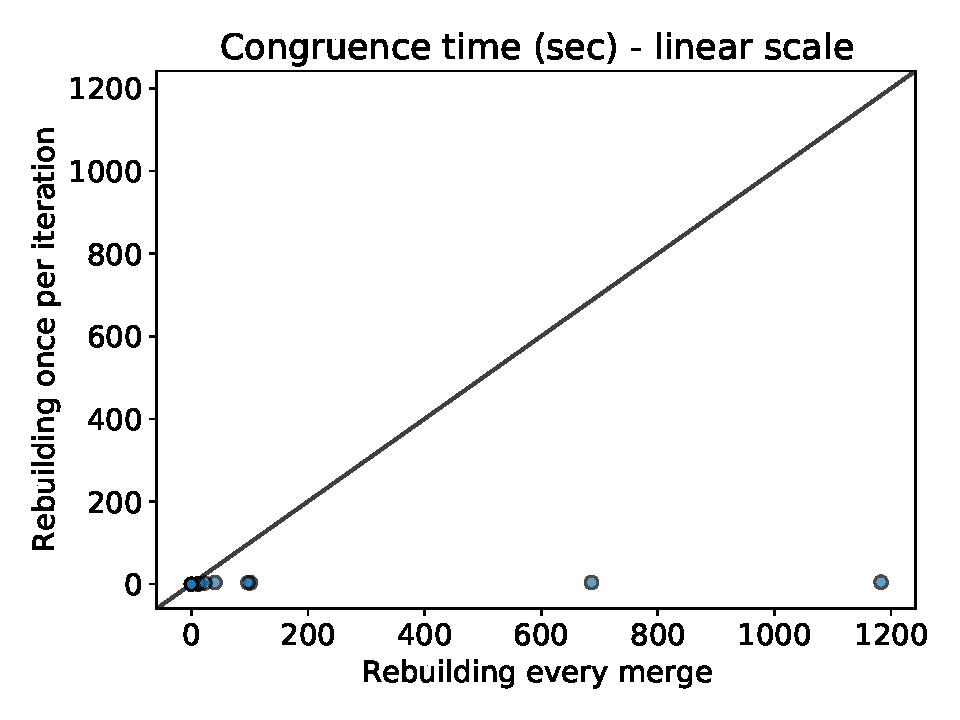
\includegraphics[height=5cm]{speedup}
  \end{subfigure}
  \hfill
  \begin{subfigure}{0.49\linewidth}
    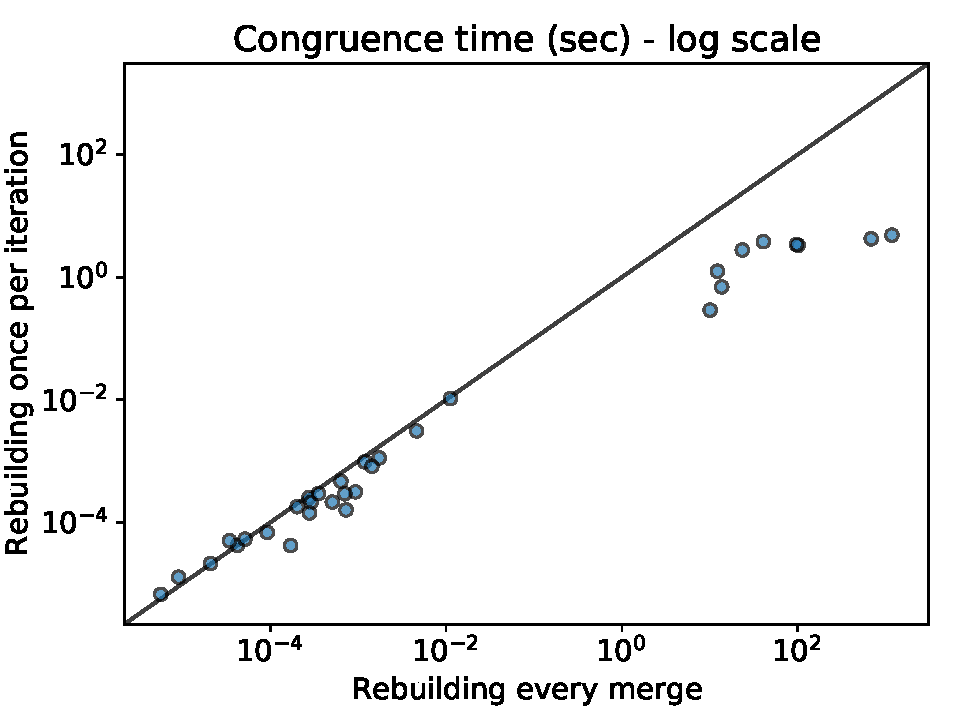
\includegraphics[height=5cm]{speedup-log}
  \end{subfigure}
  \caption{
    % 本段翻译未仔细校对
    % Rebuilding once per iteration---as opposed to after every merge---significantly
    %   speeds up congruence maintenance.
    % Both plots show the same data: one point for each of the \nEggTests tests.
    % The diagonal line is $y=x$;
    %   points below the line mean deferring rebuilding is faster.
    % In aggregate over all tests (using geometric mean),
    %   congruence is \CongrSpeedup faster, and
    %   equality saturation is \TotalSpeedup faster.
    % The linear scale plot shows that deferred rebuilding is significantly faster.
    % The log scale plot suggests the speedup is greater than some constant multiple;
    %   \autoref{fig:eval-iter} demonstrates this in greater detail.
    每次迭代只重建一次——而不是每次合并后——可显著加快同构维护。
    两个图显示相同的数据: 每个 \nEggTests 测试一个点。
    对角线是 $y=x$; 点在线下面意味着推迟重建更快。
    在所有测试中的总和(使用几何平均值), 同构快 \CongrSpeedup,等式饱和快 \TotalSpeedup。
    线性尺度图显示推迟重建显著更快。
    对数尺度图表明加速比某些常数倍大; 
      \autoref{fig:eval-iter}更详细地展示这一点。
  }
  \label{fig:eval}

  \begin{minipage}[t]{0.48\linewidth}
  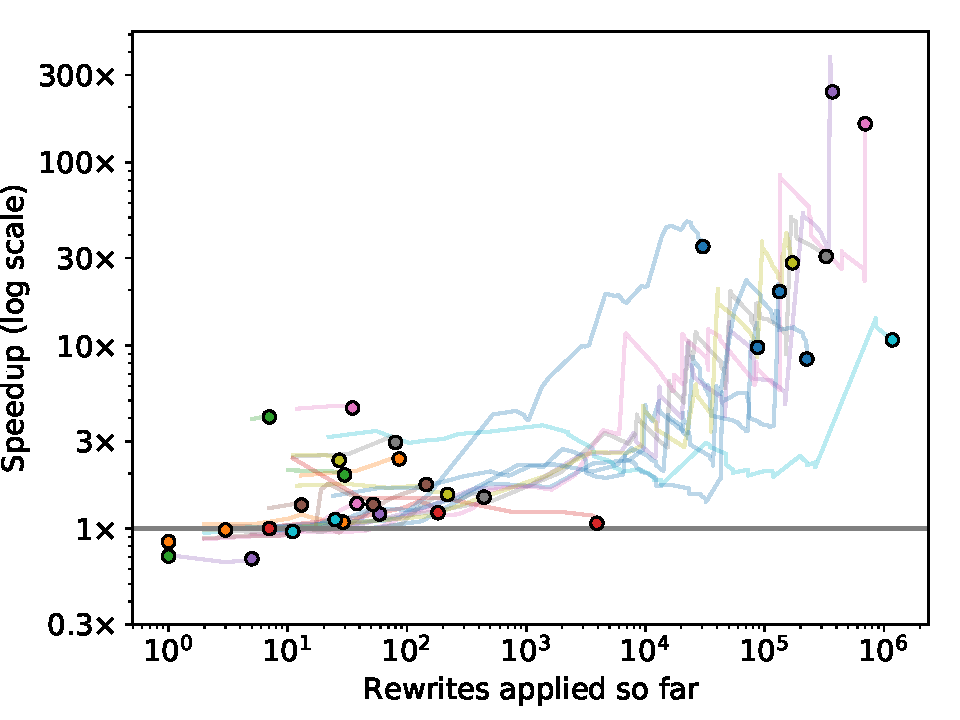
\includegraphics[height=5cm]{speedup-iter}
  \caption{
    % 本段翻译未仔细校对
    % As more rewrites are applied, deferring rebuilding gives greater speedup.
    % Each line represents a single test: each equality saturation iteration plots
    %   the cumulative rewrites applied so far against the multiplicative speedup
    %   of deferring rebuilding; the dot represents the end of that test.
    % Both the test suite as a whole (the dots) and individual tests (the lines)
    %   demonstrate an asymptotic speedup that increases with
    %   the problem size.
    当应用更多重写时,推迟重建会带来更大的加速。
    每条线表示一个测试:
      每次等式饱和迭代绘制目前已经应用的累计重写与推迟重建的乘法加速率; 
      点表示该测试结束。
    整个测试套件(点)和单独的测试(线)均表明随着问题规模的增大而增加的渐近加速。
  }
  \label{fig:eval-iter}
  \end{minipage}
  \hfill
  \begin{minipage}[t]{0.48\linewidth}
  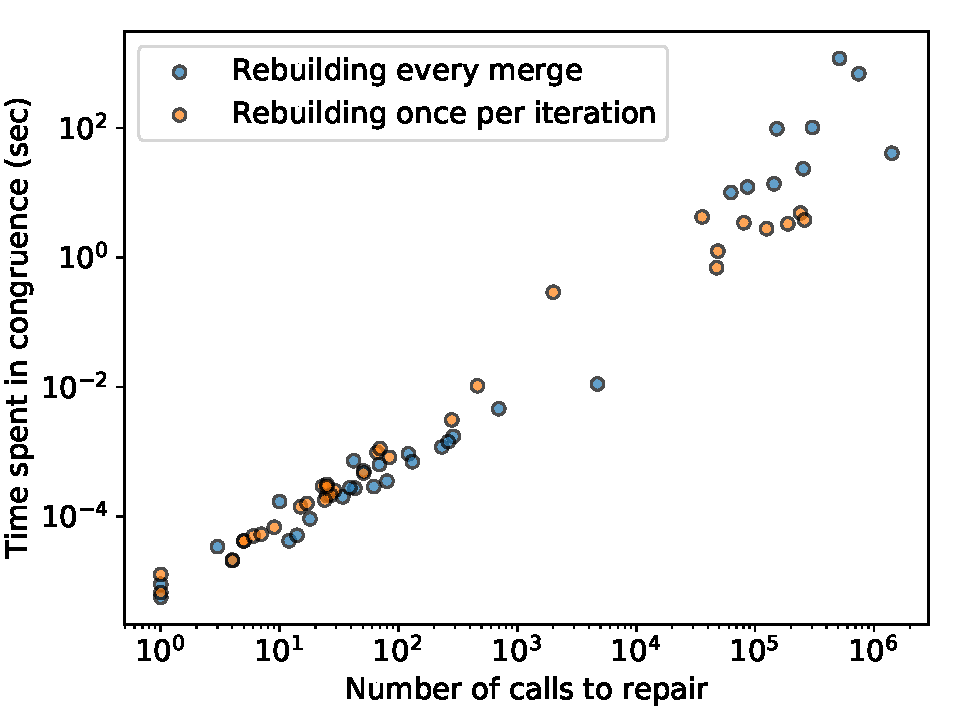
\includegraphics[height=5cm]{repairs}
  \caption{
    % 本段翻译未仔细校对
    % The time spent in congruence maintenance correlates with the number of calls
    % to the \texttt{repair} method.
    % Spearman correlation yields $r=\RepairsR$ with a p-value of \RepairsP,
    % indicating that the two quantities are indeed positively correlated.
    同构维护中的时间与\texttt{repair}方法的调用次数相关。
    Spearman 相关系数为 $r=\RepairsR$,p值为 \RepairsP,
      表明这两个量确实是正相关的。
  }
  \label{fig:repair-plot}
  \end{minipage}
\end{figure}


% 本段翻译未仔细校对
% We ran \egg's test suite using both rebuild strategies, measuring the time spent
%   on congruence maintenance.
% Each test consists of one run of \egg's equality saturation algorithm to optimize
%   a given expression.
% Of the \nEggTests total tests,
%   \nEggTimeouts hit the iteration limit of 100 and the remainder saturated.
% Note that both rebuilding strategies use \egg's phase-split equality saturation
%   algorithm, and the resulting \egraphs are identical in all cases.
% These experiments were performed on a 2020 Macbook Pro with a 2 GHz quad-core
%   Intel Core i5 processor and 16GB of memory.
我们使用两种重建策略运行了 \egg 的测试套件,并测量了在同余维护上花费的时间。
每个测试都包括一次 \egg 的等式饱和算法,以优化给定表达式。
在总共 \nEggTests 的测试中,
\nEggTimeouts 达到了100次迭代的限制,其余达到了饱和状态。
请注意,两种重建策略均使用 \egg 的分阶段等式饱和算法,并且所有情况下的 \egraphs 都是相同的。
这些实验在带有 2 GHz 四核 Intel Core i5 处理器和 16GB 内存的 2020 Macbook Pro 上进行。

% 本段翻译未仔细校对
% \autoref{fig:eval} shows our how rebuilding speeds up congruence maintenance.
% Overall, our experiments show an aggregate \CongrSpeedup speedup on congruence
%   closure and \TotalSpeedup speedup over the entire equality saturation
%   algorithm.
% \autoref{fig:eval-iter} shows this speedup is asymptotic;
%   the multiplicative speedup increases as problem gets larger.
图 \autoref{fig:eval} 显示了重建如何加速同余维护。
总体而言,我们的实验显示整体上同余闭包上有 \CongrSpeedup 加速,
  整个等式饱和算法上有 \TotalSpeedup 加速。
图 \autoref{fig:eval-iter} 显示这种加速是渐近的,随着问题规模变得更大,乘法加速率增加。


% \egg's test suite consists of two main applications:
% \texttt{math},
%   a small computer algebra system capable of symbolic differentiation and
%   integration; and
% \texttt{lambda},
%   a partial evaluator for the untyped lambda calculus using explicit
%   substitution to handle variable binding (shown in \autoref{sec:impl}).
% Both are typical \egg applications primarily driven by
%   syntactic rewrites, with a few key uses of \egg's more complex features
%   like \eclass analyses and dynamic/conditional rewrites.
\egg 的测试套件由两个主要应用组成:
\texttt{math},
一个小型计算机代数系统,能够进行符号导数和积分;
\texttt{lambda},
  一个无类型 lambda 演算的部分解释器,使用显式替换来处理变量绑定
  (如 \autoref{sec:impl} 所示)。
这两者都是典型的 \egg 应用,主要由语法重写驱动,
  并使用了 \egg 复杂的关键功能,如 \eclass 分析和动态或条件重写。


% \egg can be configured to capture various metrics about equality saturation as
%   it runs, including the time spent in the read phase (searching for matches),
%   the write phase (applying matches), and rebuilding.
% In \autoref{fig:eval}, congruence time is measured as the time spent
%   applying matches plus rebuilding.
% Other parts of the equality saturation algorithm (creating the initial \egraph,
%   extracting the final term) take negligible take compared to the equality
%   saturation iterations.
可以配置 \egg 来捕获运行过程中等式饱和的各种度量,
  包括读取阶段(搜索匹配)、写入阶段(应用匹配)和重建阶段的花费时间。
在 \autoref{fig:eval} 中,同余时间被测量为应用匹配和重建的时间。  % 同余? 下面的同余也有疑问
等式饱和算法的其他部分(创建初始 \egraph,提取最终项)与等式饱和迭代相比花费非常小。


% Deferred rebuilding amortizes the examination of \eclasses
%   for congruence maintenance;
%   deduplicating the worklist reduces the number of calls to the \texttt{repair}.
% \autoref{fig:repair-plot} shows that time spent in congruence is correlated with
%   the number of calls to the \texttt{repair} methods.
推迟重建对 \eclasses 的同余维护检查进行了摊销;
  去重工作列表减少了对 \texttt{repair} 的调用次数。
\autoref{fig:repair-plot} 显示,同余中的时间与\texttt{repair}方法的调用次数相关。


% The case study in \autoref{sec:herbie} provides a further evaluation of
%   rebuilding. Rebuilding (and other \egg features) have also been implemented in
%   a Racket-based \egraph, demonstrating that rebuilding is a conceptual advance
%   that need not be tied to the \egg implementation.
在 \autoref{sec:herbie} 中的案例研究进一步评估了重建。
  重建(和其他 \egg 特性)也已经在基于 Racket 的 \egraph 中实现,
  演示重建是为了概念推进,不用与 \egg 实现相关联。 %?

%%% Local Variables:
%%% TeX-master: "egg"
%%% End:

\section{用 \eclass 分析器拓展 \Egraphs}
% \section{Extending \Egraphs with \Eclass Analyses}
\label{sec:extensions}

% As discussed so far, \egraphs and equality saturation provide an efficient way
%   to implement a term rewriting system.
% Rebuilding enhances that efficiency, but the approach remains designed for
%   purely syntactic rewrites.
% However, program analysis and optimization typically require more than just
%   syntactic information.
正如迄今为止所讨论的,\egraphs 和 等式饱和 提供了一种高效的方法来实现一个项重写系统。
重建增强了效率,但该方法仍然仅限于语法重写。
然而,程序分析和优化通常需要的不仅仅是语法信息。
% Instead, transformations are \emph{computed} based on the input terms and also semantic facts
%   about that input term, e.g., constant value, free variables, nullability,
%   numerical sign, size in memory, and so on.
% The ``purely syntactic'' restriction has forced existing equality saturation
%   applications~\cite{eqsat, eqsat-llvm, herbie} to
%   resort to ad hoc passes over the \egraph
%   to implement analyses like constant folding.
% These ad hoc passes require manually manipulating the \egraph,
%   the complexity of which could prevent the implementation of more sophisticated
%   analyses.
%   % naturally expressed in the more conventional term rewriting setting,
%   % but must implemented as complicated \textit{ad hoc} passes over the \egraph.
相反,转换的 \emph{计算} 是基于输入 项 和该输入 项 的语义论据(semantic facts),
  例如,常量值,自由变量,空属性,数字符号,内存大小等。
“纯语法”限制迫使现有的 等式饱和 应用~\cite{eqsat, eqsat-llvm, herbie} 
  不得不求助于临时措施通过 \egraph 来实现常量折叠等分析。
这些临时措施需要手动操纵 \egraph ,其复杂性可能会妨碍实施更复杂的分析。


% We present a new technique called \textit{\eclass analysis},
%   which allows the concise
%   expression of a program analysis over the \egraph.
% An \eclass analysis resembles abstract interpretation
%   lifted to the \egraph level,
%   attaching \textit{analysis data} from a semilattice to each \eclass.
% The \egraph maintains and propagates this data as
%   \eclasses get merged and new \enodes are added.
% Analysis data can be used directly to modify the \egraph, to inform
%   how or if rewrites apply their right-hand sides, or to determine the cost of
%   terms during the extraction process.
我们提出了一种新技术,称为 \textit{\eclass 分析器(\eclass Analyses)},它允许在 \egraph 上简洁地表达程序分析。
一个 \eclass 分析器类似于提升到 \egraph 层面的抽象解释,
  从半格(semilattice)到每个\eclass 附加 \textit{分析数据}。% ?semilattice
在合并 \eclasses 和添加新的 \enodes 时,\egraph 会维护和传播这些数据。
分析数据可以直接用于修改 \egraph,以告知重写如何或是否应用其右右部,或在萃取过程中确定项的成本。

% \Eclass analyses provide a general mechanism to replace what previously
%   required ad hoc extensions that manually manipulate the \egraph.
% \Eclass analyses also fit within the equality saturation workflow,
%   so they can naturally cooperate with the equational reasoning provided by
%   rewrites.
% Moreover, an analysis lifted to the \egraph level automatically benefits from a
%   sort of ``partial-order reduction'' for free:
%   large numbers of similar programs may be analyzed for little additional cost
%   thanks to the \egraph's compact representation.
\eclass 分析器提供了一种通用机制,用来替换以前需要手动操纵 \egraph 的特殊扩展。
\eclass 分析器也适合 等式饱和 工作流程,
  因此它们可以自然地与重写提供的等式推理(equational reasoning)协作。
此外,在 \egraph 层面的分析会自动从一种“偏序归约(partial-order reduction)”中免费受益:
  借由 \egraph 的紧凑表示,大量类似程序可以以用很少的额外成本进行分析。

% This section provides a conceptual explanation of \eclass analyses as well
%   as dynamic and conditional rewrites that can use the analysis data.
% The following sections will provide concrete examples:
%   \autoref{sec:impl} discusses the \egg implementation and a complete example of a
%   partial evaluator for the lambda calculus;
%   \autoref{sec:case-studies} discusses how three published projects have used
%   \egg and its unique features (like \eclass analyses).
本节提供了 \eclass 分析器的概念解释以及可以使用分析数据的动态和条件重写。
接下来的章节将提供具体示例:
  \autoref{sec:impl} 讨论 \egg 实现和 lambda 演算中部分求值器的完整示例;
  \autoref{sec:case-studies} 讨论三个已发布项目如何使用
  \egg 及其独特特性(如 \eclass 分析器)。

% 原文注释 begin
% An \eclass analysis may,  modify the \egraph itself to inject new based on the computed data,
% In this way, the \eclass analysis can work with the rewrites as opposed

% \Egg offers many convenient ways to interact with the \egraph that are difficult
%   or impossible in other implementations.
% These tools give \egg the flexibility highlighted by the diverse case studies
%   in \autoref{sec:case-studies}
%   and the lambda calculus example in \autoref{sec:lambda}.

% Like the rest of \egg, these extensions are generic over the language and
%   rewrites that the user is working with.
% These are all novel in practice, as \egg is the first (to our knowledge)
%   general-purpose, reusable \egraph library.
% \Eclass analyses appear to be conceptually novel as well.

% \Chandra{this entire section is a bit light in details and doesn't
% always connect back to the goals of egg the right way. For example,
% without a concrete advantage of runners, it's not clear why it is useful.}
% 原文注释 end

% \subsection{\Eclass Analyses}
\subsection{\eclass 分析器}
\label{sec:analysis}

% An \eclass analysis defines a domain $D$ and associates a value $d_{c} \in D$ to
%   each \eclass $c$.
% The \eclass $c$ contains the associated data $d_{c}$,
%   i.e., given an \eclass $c$, one can get $d_{c}$ easily, but not vice-versa.
\eclass 分析器(\eclass Analyses)定义了一个域 $D$ 并将一个值 $d_{c} \in D$ 与每个 \eclass $c$ 关联。
\eclass $c$ 包含关联数据 $d_{c}$,
  即,给定一个 \eclass $c$,可以很容易地获得 $d_{c}$,但反过来不行。

% The interface of an \eclass analysis is as follows,
%   where $G$ refers to the \egraph,
%   and $n$ and $c$ refer to \enodes and \eclasses within $G$:
\eclass 分析器的接口如下,
  其中 $G$ 指的是 \egraph,
  $n$ 和 $c$ 指的是 $G$ 中的 \enodes 和 \eclasses :

% 原文注释 begin
% We will use the following metavariables and syntax in this section:

% \begin{center}
%   $G$: \egraph, $c$: \eclass, $n$: \enode,
%   $d_{c}$: the analysis data associated with \eclass $c$
% \end{center}
% 原文注释 end

% 本段翻译未仔细校对
\vspace{1em}
\begin{tabular}{lp{0.7\linewidth}}
  $\textsf{make}(n) \to d_{c}$ &
    % When a new \enode $n$ is added to $G$ into a new, singleton \eclass $c$,
    % construct a new value $d_{c} \in D$ to be associated with $n$'s new \eclass,
    % typically by accessing the associated data of $n$'s children.
    当一个新的 \enode $n$ 被添加到 $G$ 并且形成一个新的,单一的 \eclass $c$ 时,
    构造一个新值 $d_{c} \in D$ 与 $n$ 的新 \eclass 关联,
    通常通过访问 $n$ 的子节点的关联数据。
  \\
  $\textsf{join}(d_{c_1}, d_{c_2}) \to d_{c}$ &
    % When \eclasses $c_{1}, c_{2}$ are being merged into $c$,
    % join $d_{c_1}, d_{c_2}$ into a new value $d_{c}$ to be associated with the
    % new \eclass $c$.
    当 \eclasses $c_{1}, c_{2}$ 被合并成 $c$ 时,将 $d_{c_1}, d_{c_2}$ 合并成一个新值 $d_{c}$ 与新 \eclass $c$ 关联。
  \\
  $\textsf{modify}(c) \to c'$ &
    % Optionally modify the \eclass $c$ based on $d_{c}$, typically by adding an
    %   \enode to $c$.
    % Modify should be idempotent if no other changes occur to the \eclass, i.e.,
    %   $\textsf{modify}(\textsf{modify}(c)) = \textsf{modify}(c)$
    % % Returning $c$ unmodified ($c = c'$) suffices in many cases, and is the
    % % default implementation for analyses in \egg.
    根据 $d_{c}$ 可选地修改 \eclass $c$,通常是添加一个 \enode 到 $c$。
    如果 \eclass 没有其他变化,修改应该幂等,即 
      $\textsf{modify}(\textsf{modify}(c)) = \textsf{modify}(c)$
\end{tabular}
\vspace{1em}

% The domain $D$ together with the \textsf{join} operation should form a join-semilattice.
% The semilattice perspective is useful for defining the \textit{analysis invariant}
%   (where $\wedge$ is the \textsf{join} operation):
域 $D$ 与 \textsf{join} 操作一起应该形成一个联并半格(join-semilattice)。 % ?
半格视角对于定义 \textit{分析不变量} 是很有用的。 % ?
  (其中 $\wedge$是textsf{join}操作)。
\[
  \forall c \in G.\quad
  d_{c} = \bigwedge_{n \in c} \textsf{make}(n)
  \quad \text{and} \quad
  \textsf{modify}(c) = c
\]

% 本段翻译未仔细校对
% The first part of the analysis invariant states that the data associated with
%   each \eclass must be the \textsf{join} of the \textsf{make} for every \enode
%   in that \eclass.
% Since $D$ is a join-semilattice, this means that
%   $\forall c, \forall n \in c, d_{c} \geq \textsf{make}(n) $.
% The motivation for the second part is more subtle.
% Since the analysis can modify an \eclass through the \textsf{modify} method,
%   the analysis invariant asserts that these modifications are driven to a fixed
%   point.
% When the analysis invariant holds, a client looking at the analysis data can be
%   assured that the analysis is ``stable'' in the sense that
%   recomputing \textsf{make}, \textsf{join}, and \textsf{modify} will not
%   modify the \egraph or any analysis data.
第一部分的分析不变性声明,
  每个 \eclass 的关联的数据必须是每个 \enode 的 \textsf{make} 的\textsf{join}。
由于 $D$ 是 联并半格(join-semilattice) ,这意味着
  $\forall c, \forall n \in c, d_{c} \geq \textsf{make}(n) $。
第二部分的动机更为微妙。
由于分析可以通过 \textsf{modify} 方法修改一个\eclass,
  分析不变性声明这些修改被驱动到一个固定点。
当分析不变性成立时,客户端看到的分析数据可以确保分析在重新计算
  \textsf{make},\textsf{join},\textsf{modify} 不会修改 \egraph 或任何分析数据的意义下是“稳定”的。

% \subsubsection{Maintaining the Analysis Invariant}
\subsubsection{保持分析不变量(Analysis Invariant)}

% 因模板问题,代码注释暂不翻译
\begin{figure}
  \begin{minipage}[t]{0.47\linewidth}
    \begin{lstlisting}[gobble=4, numbers=left, numberstyle=\color{black}, basicstyle=\scriptsize\ttfamily\color{black!40}, escapechar=|]
    def add(enode):
      enode = self.canonicalize(enode)
      if enode in self.hashcons:
        return self.hashcons[enode]
      else:
        eclass = self.new_singleton_eclass(enode)
        for child_eclass in enode.children:
          child_eclass.parents.add(enode, eclass)
        self.hashcons[enode] = eclass
        |\color{black}\label{line:add1} eclass.data = analysis.make(enode)|
        |\color{black}\label{line:add2} analysis.modify(eclass)|
        return eclass

    def merge(eclass1, eclass2)
      union = self.union_find.union(eclass1, eclass2)
      if not union.was_already_unioned:
        |\color{black}\label{line:merge1}d1, d2 = eclass1.data, eclass2.data|
        |\color{black}\label{line:merge2}union.eclass.data = analysis.join(d1, d2)|
        self.worklist.add(union.eclass)
      return union.eclass
    \end{lstlisting}
  \end{minipage}
  \hfill
  \begin{minipage}[t]{0.47\linewidth}
    \begin{lstlisting}[gobble=4, numbers=left, firstnumber=21, numberstyle=\color{black}, basicstyle=\scriptsize\ttfamily\color{black!40}, escapechar=|]
    def repair(eclass):
      for (p_node, p_eclass) in eclass.parents:
        self.hashcons.remove(p_node)
        p_node = self.canonicalize(p_node)
        self.hashcons[p_node] = self.find(p_eclass)

      new_parents = {}
      for (p_node, p_eclass) in eclass.parents:
        p_node = self.canonicalize(p_node)
        if p_node in new_parents:
          self.union(p_eclass, new_parents[p_node])
        new_parents[p_node] = self.find(p_eclass)
      eclass.parents = new_parents
    \end{lstlisting}
    \vspace{-3mm}
    \begin{lstlisting}[gobble=4, numbers=left, firstnumber=34, basicstyle=\scriptsize\ttfamily, escapechar=|]

      # 任何对 eclass 的修改
      # 都会添加到 worklist 中
      |\label{line:repair1}|analysis.modify(eclass)
      for (p_node, p_eclass) in eclass.parents:
        new_data = analysis.join(
          p_eclass.data,
          analysis.make(p_node))
        if new_data != p_eclass.data:
          p_eclass.data = new_data
          |\label{line:repair2}|self.worklist.add(p_eclass)
    \end{lstlisting}
  \end{minipage}
  \caption{
    % The pseudocode for maintaining the \eclass analysis invariant is largely
    %   similar to how rebuilding maintains congruence closure
    %   (\autoref{sec:rebuilding}).
    % Only lines \ref{line:add1}--\ref{line:add2},
    %   \ref{line:merge1}--\ref{line:merge2},
    %   and \ref{line:repair1}--\ref{line:repair2} are added.
    % Grayed out or missing code is unchanged from \autoref{fig:rebuild-code}.
    维护 \eclass 分析器不变量的伪代码大体上与重建维持同余闭包的方式相似(\autoref{sec:rebuilding})。
      只添加了行 \ref{line:add1}--\ref{line:add2},
      \ref{line:merge1}--\ref{line:merge2},
      和 \ref{line:repair1}--\ref{line:repair2} 。
    灰色或未列出的代码与 \autoref{fig:rebuild-code} 相同。
    % 【代码注释翻译】
    %   # any mutations modify makes to eclass
    %   # will add to the worklist
    %   任何对 eclass 的修改
    %   都会添加到 worklist 中
  }
  \label{fig:rebuild-analysis}
\end{figure}

% 本段翻译未仔细校对
% We extend the rebuilding procedure from \autoref{sec:rebuilding} to restore the
%   analysis invariant as well as the congruence invariant.
% \autoref{fig:rebuild-analysis} shows the necessary modifications to the
%   rebuilding code from \autoref{fig:rebuild-code}.
我们将重建过程从 \autoref{sec:rebuilding} 扩展到恢复分析不变性和同余不变性。
\autoref{fig:rebuild-analysis}显示了从\autoref{fig:rebuild-code}修改重建代码所需的修改。


% 本段翻译未仔细校对
% Adding \enodes and merging \eclasses risk breaking the analysis invariant in
%   different ways.
% Adding \enodes is the simpler case; lines \ref{line:add1}--\ref{line:add2}
%   restore the invariant for the newly created, singleton \eclass that holds the
%   new \enode.
% When merging \enodes, the first concern is maintaining the semilattice portion of the
%   analysis invariant.
% Since \textsf{join} forms a semilattice over the domain $D$ of the analysis
%   data, the order in which the joins occur does not matter.
% Therefore, line \ref{line:merge2} suffices to update the analysis data of the
%   merged \eclass.
添加 \enodes 和合并 \eclasses 都有可能以不同的方式打破分析不变性。
添加\enodes 是更简单的情况;
  行 \ref{line:add1}--\ref{line:add2} 恢复了新创建的,单个 \eclass 的不变性。%?singleton
合并\enodes 时,第一个关注点是维护分析不变性的半阶部分。
由于\textsf{join}在分析数据的域D上形成半阶,因此合并的顺序并不重要。
因此,线\ref{line:merge2}足以更新合并的\eclass 的分析数据。

% 本段翻译未仔细校对
% Since $\textsf{make}(n)$ creates analysis data by looking at the data of $n$'s,
%   children, merging \eclasses can violate the analysis invariant in the same way
%   it can violate the congruence invariant.
% The solution is to use the same worklist mechanism introduced in
%   \autoref{sec:rebuilding}.
% Lines \ref{line:repair1}--\ref{line:repair2} of the \texttt{repair} method
%   (which \texttt{rebuild} on each element of the worklist)
%   re-\textsf{make} and \textsf{merge} the analysis data of the parent of any
%   recently merged \eclasses.
% The new \texttt{repair} method also calls \textsf{modify} once, which suffices
%   due to its idempotence.
% In the pseudocode, \textsf{modify} is reframed as a mutating method for clarity.
由于 $\textsf{make}(n)$ 通过查看 $n$ 的子元素创建分析数据,
  因此合并 \eclasses 可能会在同一方式中违反分析不变性。
解决方案是使用在 \autoref{sec:rebuilding} 中引入的相同工作列表机制。
\texttt{repair} 方法 (它在工作列表的每个元素上\texttt{rebuild}) 
  的行 \ref{line:repair1}--\ref{line:repair2} 
  重新 \textsf{make}和 \textsf{merge} 最近合并的 \eclasses 父元素的分析数据。
新的 \texttt{repair} 方法还调用 \textsf{modify} 一次,这足以满足其幂等性(idempotence)。
在伪代码中,为了更明晰,\textsf{modify} 被重构为一种可变方法。


% 本段翻译未仔细校对
% \Egg's implementation of \eclass analyses assumes that the analysis domain $D$
%   is indeed a semilattice and that \textsf{modify} is idempotent.
% Without these properties, \egg may fail to restore the analysis invariant on
%   \texttt{rebuild}, or it may not terminate.
\Egg 实现的 \eclass 分析器假设分析域 $D$ 确实是半格,
  并且 \textsf{modify} 具有幂等性。
如果没有这些性质,\egg 可能无法在 \texttt{rebuild} 上恢复分析不变量,或者它可能永不终止。

% % \subsubsection{Modifying the \Egraph from an \Eclass Analysis}
% \subsubsection{Example: Constant Folding}
\subsubsection{示例: 常量折叠(Constant folding)}


% 本段翻译未仔细校对
% The data produced by \eclass analyses can be
%   usefully consumed by other components of an equality saturation system
%   (see \autoref{sec:rewrites}),
%   but \eclass analyses can be useful on their own thanks to the
%   \textsf{modify} hook.
% Typical \textsf{modify} hooks will either do nothing, check some invariant about
%   the \eclasses being merged, or add an \enode to that \eclass
%   (using the regular \texttt{add} and \texttt{merge} methods of the \egraph).
\eclass 分析器产生的数据可以被其他 等式饱和 系统组件有效地使用(参见 \autoref{sec:rewrites}),
但是由于 \textsf{modify} 钩子的存在,\eclass 分析器可以独立使用
典型的 \textsf{modify} 钩子 会什么事都不做,检查要合并的 \eclasses 的某些不变量,
或者将一个 \enode 添加到该 \eclass 中(使用 \egraph 的常规 \texttt{add} 和 \texttt{merge} 方法)。

% 本段翻译未仔细校对
% As mentioned above, other equality saturation implementations have implemented
%   constant folding as custom, ad hoc passes over the \egraph.
% We can formulate constant folding as an \eclass analysis that highlights the
%   parallels with abstract interpretation.
% Let the domain $D = \texttt{Option<Constant>}$, and let the \texttt{join}
%   operation be the ``\texttt{or}'' operation of the \texttt{Option} type:
如上所述,其他 等式饱和 实现已经将常量折叠实现为自定义的,
  临时通过 \egraph 的步骤。 %?
我们可以将常量折叠表示为一个 \eclass 分析器,突出了它与抽象解释之间的相似之处。
设域 $D = \texttt{Option<Constant>}$,
  设 \texttt{join} 操作是 \texttt{Option} 类型上的 ``\texttt{or}'' 操作:  
\\
\begin{minipage}{\linewidth}
\begin{lstlisting}[language=Rust, basicstyle=\ttfamily\footnotesize, xleftmargin=35mm]
match (a, b) {
  (None,    None   ) => None,
  (Some(x), None   ) => Some(x),
  (None,    Some(y)) => Some(y),
  (Some(x), Some(y)) => { assert!(x == y); Some(x) }
}
\end{lstlisting}
\end{minipage}
\\
% 本段翻译未仔细校对
% Note how \textsf{join} can also aid in debugging by checking properties about
%   values that are unified in the \egraph;
%   in this case we assert that all terms represented in an \eclass should have
%   the same constant value.
% The \textsf{make} operation serves as the abstraction function, returning the
%   constant value of an \enode if it can be computed from the constant values
%   associated with its children \eclasses.
% The \textsf{modify} operation serves as a concretization function in this
%   setting.
% If $d_{c}$ is a constant value, then $\textsf{modify}(c)$ would add
%   $\gamma(d_{c}) = n$ to $c$, where $\gamma$ concretizes the constant value into
%   a childless \enode.
注意如何 \textsf{join} 也可以通过检查在 \egraph 中统一的值的属性来辅助调试;
  在这种情况下,我们断言在 \eclass 中表示的所有项应该具有相同的常量值。
\textsf{make} 操作充当抽象函数,
  如果它可以从与其子\eclasses 相关联的常量值计算出来,
  返回 \enode 的常量值。
\textsf{modify} 操作在这个设置中充当具体化函数。 %  concretization?
如果 $d_{c}$ 是一个常量值,那么 $\textsf{modify}(c)$ 就会将 
  $\gamma(d_{c}) = n$ 添加到 $c$ 中,
  其中 $\gamma$ 将常量值具体化(concretizes)为没有子节点的 \enode。

% 本段翻译未仔细校对
% Constant folding is an admittedly simple analysis, but one that did not formerly
%   fit within the equality saturation framework.
% \Eclass analyses support more complicated analyses in a general way, as
%   discussed in later sections on the \egg implementation and case studies
%   (Sections \ref{sec:impl} and \ref{sec:case-studies}).
常量折叠是一种明显简单的分析,但之前并不适合 等式饱和 框架。
\Eclass analyses 在通用的方式中支持更复杂的分析,
  如后面关于 \egg 实现和案例研究的章节所讨论的
  (\ref{sec:impl} 和 \ref{sec:case-studies})。

% \subsection{Conditional and Dynamic Rewrites}
\subsection{条件和动态重写}
\label{sec:rewrites}

% 此段翻译未仔细校对
% In equality saturation applications, most of the rewrites are purely
%   syntactic.
% In some cases, additional data may be needed to determine if or how to perform
%   the rewrite.
% For example, the rewrite $x / x \to 1$ is only valid if $x \neq 0$.
% A more complex rewrite may need to compute the right-hand side dynamically based
%   on an analysis fact from the left-hand side.
在 等式饱和 应用中,大多数重写都是纯粹的语法形式。
在某些情况下,可能需要额外的数据来确定是否执行重写或如何执行重写。
例如,$x / x \to 1$ 重写仅在 $x \neq 0$ 时有效。
更复杂的重写可能需要根据左侧的分析事实动态计算右侧。

% 此段翻译未仔细校对
% The right-hand side of a rewrite can be generalized to a function
%   \textsf{apply} that takes a substitution and an \eclass generated from
%   e-matching the left-hand side, and produces a term to be added to the \egraph
%   and unified with the matched \eclass.
% For a purely syntactic rewrite, the \textsf{apply} function need not inspect the
%   matched \eclass in any way; it would simply apply
%   the substitution to the right-hand pattern to produce a new term.
重写的右侧可以概括为函数 \textsf{apply},该函数采用替代和通过 e-matching 左侧得到的 \eclass,并产生一个项,该项将被添加到 \egraph 中并与匹配的 \eclass 统一。
对于纯粹的语法重写,\textsf{apply} 函数无需以任何方式检查匹配的 \eclass;它只需将替代应用于右侧模式以产生新术语即可。

% 此段翻译未仔细校对
% \Eclass analyses greatly increase the utility of this generalized form of
%   rewriting.
% The \textsf{apply} function can look at the analysis data for the matched
%   \eclass or any of the \eclasses in the substitution to determine if or how to
%   construct the right-hand side term.
% These kinds of rewrites can broken down further into two categories:
\eclass 分析器大大增加了这种重写的通用形式的效用。
\textsf{apply} 函数可以查看匹配的 \eclass 的分析数据或替代中的任何 \eclasses,以确定如何构造右侧术语。这些重写可以进一步分为两类:
\begin{itemize}
  % \item \textit{Conditional} rewrites like $x / x \to 1$ that are purely
  % syntactic but whose validity depends on checking some analysis data;
  % \item \textit{Dynamic} rewrites that compute the right-hand side based on
  % analysis data.
  \item \textit{条件} 重写,如 $x / x \to 1$,它们是纯粹的语法形式,
    但其有效性取决于检查一些分析数据。
  \item \textit{动态} 重写,它们根据分析数据计算右侧。
\end{itemize}

% 此段翻译未仔细校对
% Conditional rewrites are a subset of the more general dynamic rewrites.
% Our \egg implementation supports both.
% The example in \autoref{sec:impl} and case studies in \autoref{sec:case-studies}
%   heavily use generalized rewrites, as it is typically the most convenient way
%   to incorporate domain knowledge into the equality saturation
%   framework.
条件重写是更一般动态重写的子集。我们的 \egg 实现支持两者。在 \autoref{sec:impl} 中的示例和在 \autoref{sec:case-studies} 中的案例研究中大量使用了广义重写,因为这通常是将领域知识纳入 等式饱和 框架的最方便的方法。

% \subsection{Extraction}
\subsection{萃取(Extraction)}
\label{sec:tricks-extraction}


% Equality saturation typically ends with an extraction phase that selects an
%   optimal represented term from an \eclass according to some cost function.
% In many domains \cite{herbie, szalinski}, AST size
%   (sometimes weighted differently for different operators) suffices as a simple,
%   local cost function.
% We say a cost function $k$ is local when the cost of a term $f(a_{1}, ...)$ can be
%   computed from the function symbol $f$ and the costs of the children.
% With such cost functions, extracting an optimal term can be efficiently done
%   with a fixed-point traversal over the \egraph that selects the minimum cost
%   \enode from each \eclass \cite{herbie}.
等式饱和通常以萃取阶段结束,该阶段根据某些成本函数从 \eclass 中选择最优表示术语。
在许多领域 \cite{herbie, szalinski} 中,
  AST(抽象语法树) 大小(有时对不同运算符的权重不同)足以作为简单的局部成本函数。 
当我们可以从函数符号 $f$ 和子结点的成本计算出术语 $f(a_{1}, ...)$ 的成本时,
  称成本函数 $k$ 为局部的。
使用这样的成本函数(cost function),从 \egraph 中萃取出最佳项可以通过固定点遍历 \egraph 在每个 \eclass 中选择具有最小代价的 \enode 来高效地完成 \cite{herbie}。

% 此段翻译未仔细校对
% Extraction can be formulated as an \eclass analysis when the cost function
%   is local.
% The analysis data is a tuple $(n, k(n))$ where $n$ is the cheapest \enode
%   in that \eclass and $k(n)$ its cost.
% The $\textsf{make}(n)$ operation calculates the cost $k(n)$ based on
%   the analysis data (which contain the minimum costs) of $n$'s children.
% The \textsf{merge} operation simply takes the tuple with lower cost.
% The semilattice portion of the analysis invariant then guarantees that the
%   analysis data will contain the lowest-cost \enode in each class.
% Extract can then proceed recursively;
%   if the analysis data for \eclass $c$ gives $f(c_{1}, c_{2}, ...)$ as the optimal \enode,
%   the optimal term represented in $c$ is
%   $\textsf{extract}(c) = f( \textsf{extract}(c_{1}), \textsf{extract}(c_{2}), ... )$.
% % The optimal term represented in an \eclass can then be built recursively,
% %   starting with the optimal \enode from the analysis data.
% % Extraction can be completed by starting from the desired \eclass and
% %   building the term recursively based on the \enode from the analysis data.
% This not only further demonstrates the generality of \eclass analyses, but also
%   provides the ability to do extraction ``on the fly''; conditional and dynamic
%   rewrites can determine their behavior based on the cheapest term in an \eclass.
萃取可以在成本函数是局部的情况下被表述为(formulated)为 \eclass 分析器。 %?formulated
分析数据是一个元组 $(n, k(n))$,其中 $n$ 是该 \eclass 中最代价最小的 \enode,
  $k(n)$ 是它的代价。
$\textsf{make}(n)$ 操作基于 $n$ 的子节点的分析数据(其中包含最小花费)计算 $k(n)$。
\textsf{merge} 操作只需取较低代价的元组。
分析不变量的半格部分(semilattice portion)保证了分析数据将包含每个类中最低花费的 \enode。
提取可以递归进行;
  如果 \eclass $c$ 的分析数据给出 $f(c_{1}, c_{2}, ...)$ 作为最佳 \enode,
  则 $c$ 表示的最佳项是  
  $\textsf{extract}(c) = f( \textsf{extract}(c_{1}), \textsf{extract}(c_{2}), ... )$。
这不仅进一步证明了 \eclass 分析器的普遍性,还提供了“即时”提取的能力;
  条件和动态重写可以根据分析数据来确定其行为。

% Extraction (whether done as a separate pass or an \eclass analysis) can also
%   benefit from the analysis data.
% Typically, a local cost function can only look at the function symbol of the
%   \enode $n$ and the costs of $n$'s children.
% When an \eclass analysis is attached to the \egraph, however, a cost function
%   may observe the data associated with $n$'s \eclass, as well as the data
%   associated with $n$'s children.
% This allows a cost function to depend on computed facts rather that just purely
%   syntactic information.
% In other words, the cost of an operator may differ based on its inputs.
% \autoref{sec:spores} provides a motivating case study wherein an \eclass
%   analysis computes the size and shape of tensors, and this size information
%   informs the cost function.
萃取(无论是作为单独的过程还是作为 \eclass 分析器)也可以从分析数据中受益。
通常,局部成本函数只能查看 \enode $n$ 的函数符号和 $n$ 的子节点的成本。
但是,当 \eclass 分析器附加到 \egraph 时,
  成本函数可以观察与 $n$ 的 \eclass 关联的数据,
  以及与 $n$ 的子节点关联的数据。
这允许成本函数依赖于计算出的论据(facts)而不仅仅是纯语法信息。
换句话说,运算符的成本可能因其输入而不同。
\autoref{sec:spores} 提供了一个激励性的案例研究(motivating case study ),% ? motivating case study 
  其中 \eclass 分析器将计算张量的大小和形状,这些大小信息会影响成本函数。

%%% Local Variables:
%%% TeX-master: "egg"
%%% End:

\section{\egg: 易用, 可拓展, 高效率的 \Egraphs}
% \section{\egg: Easy, Extensible, and Efficient \Egraphs}
% \section{\egg: implementation and strengths}
% 翻译完成

\label{sec:egg}
\label{sec:impl}
\label{sec:lambda}

% We implemented the techniques of rebuilding and \eclass analysis in \egg,
%   an easy-to-use, extensible, and efficient \egraph library.
% To the best of our knowledge,
%   \egg is the first general-purpose, reusable \egraph implementation.
% This has allowed focused effort on ease of use and optimization,
%   knowing that any benefits will
%   be seen across use cases as opposed to a single, ad hoc instance.
我们在 \egg 中实现了重构和 \eclass 分析技术,
  它是一个易于使用、可扩展、高效的 \egraph 库。
据我们所知,\egg 是第一个通用、可重用的 \egraph 实现。
这使得我们可以专注于易用性和优化,
  因为任何优点都将在不同的使用场景中体现,
  而不是仅限于一个特定的情况。

% This section details \egg's implementation and some of the various
%   optimizations and tools it provides to the user.
% We use an extended example of a partial evaluator for the lambda calculus\footnote{
%   \Egraphs do not have any ``built-in'' support for binding;
%   for example, equality modulo alpha renaming is not free.
%   The explicit substitution provided in this section is is illustrative but rather high in performance cost.
%   Better support for languages with binding is important future work.
% },
%   for which we provide the complete source code (which few changes for readability)
%   in \autoref{fig:lambda-lang} and \autoref{fig:lambda-analysis}.
% While contrived, this example is compact and familiar, and it highlights
%   (1) how \egg is used and (2) some of its novel features like
%   \eclass analyses and dynamic rewrites.
% It demonstrates how \egg can tackle binding,
%   a perennially tough problem for \egraphs,
%   with a simple explicit substitution approach
%   powered by \egg's extensibility.
% \autoref{sec:case-studies} goes further, providing real-world case studies of
%   published projects that have depended on \egg.
本节详细说明了 \egg 的实现和它为用户提供的各种优化和工具。
我们使用了一个对于 lambda 演算的部分求值器的扩展示例 \footnote{
  \Egraphs 没有任何“内置”的绑定支持;
  例如,“同模(equality modulo) 阿尔法重命名(alpha renaming)”不是无成本的。
  本节中提供的显式替换相当耗性能,未来的重要工作是更好的支持有绑定的语言。
},
  完整的源代码在 \autoref{fig:lambda-lang} 和 \autoref{fig:lambda-analysis} 中提供
  (仅做了少量修改以方便阅读)。
尽管示例稍显做作, 但它紧凑易懂, 并突出了
  (1) \egg 的使用方式和 (2) 其中一些新特性, 比如 \eclass 分析和动态重写。
它演示了如何借助 \egg 的可扩展性,比如使用简单的显式替换方法来解决绑定问题——
  这是一个对于\egraphs 来说永恒的难题。 
\autoref{sec:case-studies} 提供了更多真实世界的案例研究,
  展示了依赖 \egg 的已经发布的项目。

% \egg is implemented in \textasciitilde{}5000 lines of Rust,\footnote
% {
%   \citeauthor{rust} is a high-level systems programming language.
%   \egg has been integrated into applications written in other
%   programming languages using both C FFI and serialization approaches.
% }
% including code, tests, and documentation.
% \egg is open-source, well-documented, and distributed via Rust's package
%   management system.\footnote{
%   Source: \url{https://github.com/mwillsey/egg}.
%   Documentation: \url{https://docs.rs/egg}.
%   Package: \url{https://crates.io/crates/egg}.
% }
% All of \egg's components are generic over the
%   user-provided language, analysis, and cost functions.
\egg 由 \textasciitilde{}5000 行包括代码、测试和文档的 Rust \footnote
{
  \citeauthor{rust} 是一种高级系统编程语言。
  \egg 已经被集成到其他编程语言编写的应用程序中,使用 C FFI 和序列化方法。
}实现。
\egg 是开源的、文档齐全的, 通过 Rust 的包管理系统发布。\footnote{
  源码: \url{https://github.com/mwillsey/egg}.
  文档: \url{https://docs.rs/egg}.
  包: \url{https://crates.io/crates/egg}.
}
\egg 所有组件都是针对用户提供的语言、分析和成本函数的通用组件。

% \subsection{Ease of Use}
\subsection{易用}
\label{sec:egg-easy}

% 翻译完成
\begin{figure}
\begin{subfigure}[t]{0.48\linewidth}
  \begin{lstlisting}[language=Rust, basicstyle=\tiny\ttfamily, numbers=left, escapechar=|]
define_language! {
  enum Lambda {
    // 枚举变量具有数据或子元素(eclass Ids)
    // [Id; N] 是 N 个 Id 的数组

    // 基础类型操作符
    "+" = Add([Id; 2]), "=" = Eq([Id; 2]),
    "if" = If([Id; 3]),

    // 函数和绑定
    "app" = App([Id; 2]), "lam" = Lambda([Id; 2]),
    "let" = Let([Id; 3]), "fix" = Fix([Id; 2]),

    // (var x)是使用`x`作为表达式
    "var" = Use(Id),
    // (subst a x b)在 b 中替换(var x)的 a
    "subst" = Subst([Id; 3]),

    // 基础类型没有子元素,只有数据
    Bool(bool), Num(i32), Symbol(String),
  }
}

// 示例项和它们简化为的内容
// 直接从 |\egg| 测试套件中提取

test_fn! { lambda_under, rules(),
  "(lam x (+ 4 (app (lam y (var y)) 4)))"
  => "(lam x 8))",
}

test_fn! { lambda_compose_many, rules(),
  "(let compose (lam f (lam g (lam x
                (app (var f)
                     (app (var g) (var x))))))
   (let add1 (lam y (+ (var y) 1))
   (app (app (var compose) (var add1))
        (app (app (var compose) (var add1))
             (app (app (var compose) (var add1))
                  (app (app (var compose) (var add1))
                       (var add1)))))))"
  => "(lam ?x (+ (var ?x) 5))"
}

test_fn! { lambda_if_elim, rules(),
  "(if (= (var a) (var b))
       (+ (var a) (var a))
       (+ (var a) (var b)))"
  => "(+ (var a) (var b))"
}\end{lstlisting}
\end{subfigure}
\hfill
\begin{subfigure}[t]{0.48\linewidth}
  \begin{lstlisting}[language=Rust, basicstyle=\tiny\ttfamily, escapechar=|, numbers=left, firstnumber=51]
// 返回重写规则列表
fn rules() -> Vec<Rewrite<Lambda, LambdaAnalysis>> { vec![

 // open term rules 开放项规则
 rw!("if-true";  "(if  true ?then ?else)" => "?then"),
 rw!("if-false"; "(if false ?then ?else)" => "?else"),
 rw!("if-elim";  "(if (= (var ?x) ?e) ?then ?else)" => "?else"
     if ConditionEqual::parse("(let ?x ?e ?then)",
                              "(let ?x ?e ?else)")),
 rw!("add-comm";  "(+ ?a ?b)"        => "(+ ?b ?a)"),
 rw!("add-assoc"; "(+ (+ ?a ?b) ?c)" => "(+ ?a (+ ?b ?c))"),
 rw!("eq-comm";   "(= ?a ?b)"        => "(= ?b ?a)"),

 // substitution introduction 替换引入
 rw!("fix";     "(fix ?v ?e)" =>
                "(let ?v (fix ?v ?e) ?e)"),
 rw!("beta";    "(app (lam ?v ?body) ?e)" =>
                "(let ?v ?e ?body)"),

 // substitution propagation 替换传播
 rw!("let-app"; "(let ?v ?e (app ?a ?b))" =>
                "(app (let ?v ?e ?a) (let ?v ?e ?b))"),
 rw!("let-add"; "(let ?v ?e (+   ?a ?b))" =>
                "(+   (let ?v ?e ?a) (let ?v ?e ?b))"),
 rw!("let-eq";  "(let ?v ?e (=   ?a ?b))" =>
                "(=   (let ?v ?e ?a) (let ?v ?e ?b))"),
 rw!("let-if";  "(let ?v ?e (if ?cond ?then ?else))" =>
                "(if (let ?v ?e ?cond)
                     (let ?v ?e ?then)
                     (let ?v ?e ?else))"),

 // substitution elimination 替换消除
 rw!("let-const";    "(let ?v ?e ?c)" => "?c"
     if is_const(var("?c"))),
 rw!("let-var-same"; "(let ?v1 ?e (var ?v1))" => "?e"),
 rw!("let-var-diff"; "(let ?v1 ?e (var ?v2))" => "(var ?v2)"
     if is_not_same_var(var("?v1"), var("?v2"))),
 rw!("let-lam-same"; "(let ?v1 ?e (lam ?v1 ?body))" =>
                     "(lam ?v1 ?body)"),
 rw!("let-lam-diff"; "(let ?v1 ?e (lam ?v2 ?body))" =>
     ( CaptureAvoid {
        fresh: var("?fresh"), v2: var("?v2"), e: var("?e"),
        if_not_free: "(lam ?v2 (let ?v1 ?e ?body))"
                     .parse().unwrap(),
        if_free: "(lam ?fresh (let ?v1 ?e
                              (let ?v2 (var ?fresh) ?body)))"
                 .parse().unwrap(),
     })
     if is_not_same_var(var("?v1"), var("?v2"))),
]}\end{lstlisting}
\end{subfigure}
\caption[Language and rewrites for the lambda calculus in \egg]{
% \egg is generic over user-defined languages;
%   here we define a language and rewrite rules for a lambda calculus partial evaluator.
% The provided \texttt{define\_language!} macro (lines 1-22) allows the simple definition
%   of a language as a Rust \texttt{enum}, automatically deriving parsing and
%   pretty printing.
% A value of type \texttt{Lambda} is an \enode that holds either data that the
%   user can inspect or some number of \eclass children (\eclass \texttt{Id}s).
\egg 是针对用户定义语言的通用框架;
  在这里,我们为 lambda 计算的部分求值器定义了语言和重写规则。 %?lambda calculus partial evaluator
提供的 \texttt{define\_language!} 宏(行1-22)
  允许简单地将语言定义为 Rust \texttt{enum},可自动派生出解析器和产生漂亮的输出的打印器。
\texttt{Lambda} 类型的值是一个 \enode,
  它保存用户可以检查的数据或一些 \eclass 子节点(\eclass \texttt{Id}s)。

% Rewrite rules can also be defined succinctly (lines 51-100).
% Patterns are parsed as s-expressions:
%   strings from the \texttt{define\_language!} invocation (ex: \texttt{fix}, \texttt{=}, \texttt{+}) and
%   data from the variants (ex: \texttt{false}, \texttt{1}) parse as operators or terms;
%   names prefixed by ``\texttt{?}'' parse as pattern variables.
也可以简洁地定义重写规则(行51-100)。
模式被解析为 s-expressions:
  从 \texttt{define\_language!} 调用中解析的字符串
  (如: \texttt{fix}, \texttt{=}, \texttt{+})和
  从变体(variant)中解析的数据 % ? variant
  (如: \texttt{false}, \texttt{1})
  解析为运算符或项(term);% ? term
  以 ``\texttt{?}'' 为前缀的名称解析为模式变量。

% Some of the rewrites made are conditional using the
%   ``\texttt{left => right if cond}''
%   syntax.
% The \texttt{if-elim} rewrite on line 57 uses \egg's provided
%   \texttt{ConditionEqual} as a condition, only applying the right-hand side
%   if the \egraph can prove the two argument patterns equivalent.
% The final rewrite, \texttt{let-lam-diff}, is dynamic to support capture avoidance;
%   the right-hand side is a Rust value that
%   implements the \texttt{Applier} trait instead of a pattern.
% \autoref{fig:lambda-analysis} contains the supporting code for these rewrites.
其中一些重写是条件重写,使用 ``\texttt{left => right if cond}'' 语法。
在57行的 \texttt{if-elim} 重写使用 \egg 提供的
  \texttt{ConditionEqual}作为条件,
  只有在 \egraph 可以证明两个参数模式等价时才应用右式。
最终的重写 \texttt{let-lam-diff} 是动态的,用来支持捕获避免(capture avoidance);
  右边是一个实现了 \texttt{Applier} 的 trait 而不是模式的 Rust 值。% trait
\autoref{fig:lambda-analysis} 包含了这些重写的支持代码。

% We also show some of the tests (lines 27-50)
%   from \egg's \texttt{lambda} test suite.
% The tests proceed by inserting the term on the left-hand side, running
%   \egg's equality saturation, and then checking to make sure the right-hand
%   pattern can be found in the same \eclass as the initial term.
我们也展示了 \egg's \texttt{lambda} 测试套件的一些测试(行~ 27-50)。
测试的过程是在左边插入 term ,运行\egg 的 等式饱和,
  然后检查以确保右部的模式可以在与初始 term 相同的 \eclass 中找到。
}
\label{fig:lambda-rules}
\label{fig:lambda-lang}
\label{fig:lambda-examples}
\end{figure}

% 代码注释翻译:

%     // enum variants have data or children (eclass Ids)
%     // [Id; N] is an array of N `Id`s
% // 枚举变量具有数据或子元素(eclass Ids)
% // [Id; N]是 N 个 Id 的数组
%     // base type operators
% // 基础类型操作符
%     // functions and binding
% // 函数和绑定
%     // (var x) is a use of `x` as an expression
% // (var x)是使用`x`作为表达式
%     // (subst a x b) substitutes a for (var x) in b
% // (subst a x b)在 b 中替换(var x)的 a
%     // base types have no children, only data
% // 基础类型没有子元素,只有数据

% // example terms and what they simplify to
% // pulled directly from the |\egg|test suite
% 示例项和它们简化为的内容
% 直接从|\egg|测试套件中提取
% // Returns a list of rewrite rules
% 返回重写规则列表
% // open term rules
% 打开 term 规则

%%% Local Variables:
%%% TeX-master: "egg"
%%% End:


% \egg's ease of use comes primarily from its design as a library.
% By defining only a language and some rewrite rules,
%   a user can quickly
%   start developing a synthesis or optimization tool.
% Using \egg as a Rust library,
%   the user defines the language using the \texttt{define\_language!} macro
%   shown in \autoref{fig:lambda-lang}, lines 1-22.
% Childless variants in the language may contain data of user-defined types,
%   and \eclass analyses or dynamic rewrites may inspect this data.
\egg 的易用性主要来自其作为库的设计。
通过只定义一种语言和一些重写规则,用户可以快速开始开发合成或优化工具。
作为一个 Rust 库来使用 \egg ,用户可以使用 \texttt{define\_language!} 宏定义语言。
  示例见 \autoref{fig:lambda-lang} ,行1-22。
语言中的子节点为空的变量可以包含用户定义类型的数据,
  \eclass 分析或动态重写可以审查这些数据。 % ?may inspect this data.

% 原文注释:
%Defining a language is the only necessary input for \egg.
%From there, a user may create and manipulate \egraphs that hold expressions from
%  that language.
%If the user wants to perform rewrites and equality saturation, \egg provides
%  facilities for this as well.

% The user provides rewrites as shown in
%   \autoref{fig:lambda-lang}, lines 51-100.
% Each rewrite has a name, a left-hand side, and a right-hand side.
% For purely syntactic rewrites, the right-hand is simply a pattern.
% More complex rewrites can incorporate conditions or even dynamic right-hand
%   sides, both explained in the \autoref{sec:egg-extensible} and \autoref{fig:lambda-applier}.
用户可以提供重写规则,见 \autoref{fig:lambda-lang},行 51-100 。
每个重写规则都有一个名称,一个左部和一个右部.
对于纯语法重写,右部仅仅是一个模式.
更复杂的重写可以包含条件甚至是动态的右部,
  这些在 \autoref{sec:egg-extensible} 和 \autoref{fig:lambda-applier} 中有解释。

% Equality saturation workflows, regardless of the application domain,
%   typically have a similar structure:
% add expressions to an empty \egraph, run rewrites until saturation or
%   timeout, and extract the best equivalent expressions according to some cost
%   function.
% This ``outer loop'' of equality saturation involves a significant amount of
%   error-prone boilerplate:
无论应用领域如何,等式饱和工作流程通常具有相似的结构:
向空的 \egraph 添加表达式,运行重写直到饱和或超时,并根据一些代价函数提取最佳等价表达式。
这种“外循环(outer loop)”的等式饱和涉及大量的
  容易出错的繁文缛节:% ?error-prone boilerplate
% \begin{itemize}
%   \item Checking for saturation, timeouts, and \egraph size limits.
%   \item Orchestrating the read-phase, write-phase, rebuild system
%     (\autoref{fig:rebuild-code}) that makes \egg fast.
%   \item Recording performance data at each iteration.
%   \item Potentially coordinating rule execution so that expansive rules like
%     associativity do not dominate the \egraph.
%   \item Finally, extracting the best expression(s) according to a
%   user-defined cost function.
% \end{itemize}
\begin{itemize}
  \item 饱和、超时和 \egraph 大小限制的检测。
  \item 协调读取阶段、写入阶段和重建系统(\autoref{fig:rebuild-code})来加速 \egg 。
  \item 在每次迭代中记录性能数据。
  \item 潜在地协调规则的执行,
    以便像结合律(associativity)这样的扩张性(expansive)规则不会在 \egraph 中占主导地位。
  \item 最后, 根据用户定义的代价函数提取最佳表达式。
\end{itemize}

% \egg provides these functionalities through its \texttt{Runner} and
%   \texttt{Extractor} interfaces.
% \texttt{Runner}s automatically detect saturation, and can be configured to stop
%   after a time, \egraph size, or iterations limit.
% The equality saturation loop provided by \egg calls \texttt{rebuild}, so users
%   need not even know about \egg's deferred invariant maintenance.
% \texttt{Runner}s record various metrics about each iteration automatically,
%   and the user can hook into this to report relevant data.
% \texttt{Extractor}s select the optimal term from an \egraph given a
%   user-defined, local cost function.\footnote{
%     As mentioned in \autoref{sec:tricks-extraction}, extraction can be
%     implemented as part of an \eclass analysis.
%     The separate \texttt{Extractor} feature is still useful for ergonomic and
%     performance reasons.
%   }
% The two can be combined as well; users commonly record the ``best so far''
%   expression by extracting in each iteration.
\egg 通过其 \texttt{Runner} 和 \texttt{Extractor} 接口提供了这些功能。
\texttt{Runner}s 会自动检测饱和状态,并可以配置为在特定时间、\egraph 大小或迭代次数限制后停止。
由 \egg 提供的等式饱和循环会调用 \texttt{rebuild},
  因此用户甚至不需要了解 \egg 的延迟不变性(deferred invariant)维护。
\texttt{Runner}s 自动记录每次迭代的各种指标,用户可以钩入(hook)此过程以报告相关数据。
\texttt{Extractor}s 根据用户定义的局部代价函数从 \egraph 中选择最优项。\footnote{
    正如在 \autoref{sec:tricks-extraction} 中提到的,萃取可以作为 \eclass 分析的一部分实现。
    由于人性化和性能原因,独立的 \texttt{Extractor} 功能仍然有用。
  }
这两者也可以结合起来;用户通常在每次迭代中萃取来记录“到目前为止最好”的表达。

% \autoref{fig:lambda-lang} also shows \egg's \texttt{test\_fn!}
%   macro for easily creating tests (lines 27-50).
% These tests create an \egraph with the given expression, run equality saturation
%   using a \texttt{Runner}, and check to make sure the right-hand pattern can be
%   found in the same \eclass as the initial expression.
\autoref{fig:lambda-lang} 也展示了 \egg 的用于轻松创建测试的 \texttt{test\_fn!} 宏(行~27-50)。
这些测试使用给定表达式创建一个 \egraph,
  使用 \texttt{Runner} 运行 等式饱和 ,
  并检查右部的模式是否能够在与初始表达式相同的 \eclass 中找到。

% \subsection{Extensibility}
\subsection{可拓展性}
\label{sec:egg-extensible}

% For simple domains, defining a language and purely syntactic rewrites will
%   suffice.
% However, our partial evaluator requires interpreted reasoning, so we use some of
%   \egg's more advanced features like \eclass analyses and dynamic rewrites.
% Importantly, \egg supports these extensibility features as a library:
%   the user need not modify the \egraph or \egg's internals.
对于简单的领域,定义语言和纯语法重写就足够了。
但是,我们的部分评估器需要解释性推理,因此我们使用了一些 \egg 更高级的功能,如 \eclass 分析和动态重写。
重要的是,\egg 作为库支持这些可扩展性功能:用户无需修改 \egraph 或 \egg 的内部。

% 翻译完成;代码注释未翻译
\begin{figure}
\begin{minipage}[t]{0.49\linewidth}
  \begin{lstlisting}[language=Rust, basicstyle=\tiny\ttfamily, numbers=left]
type EGraph = egg::EGraph<Lambda, LambdaAnalysis>;
struct LambdaAnalysis;
struct FC {
  free: HashSet<Id>,    // 我们的分析数据存储自由变量
  constant: Option<Lambda>, // 以及常量值(如果有)
}

// 帮助函数,用于制作模式元变量(pattern meta-variables)
fn var(s: &str) -> Var { s.parse().unwrap() }

impl Analysis<Lambda> for LambdaAnalysis {
  type Data = FC; // 将 FC 附加到每个 eclass
  // merge 通过合并到 “to” 实现半格联并 (semilattice join)
  // 如果 “to” 数据被修改,则返回 true
  fn merge(&self, to: &mut FC, from: FC) -> bool {
    let before_len = to.free.len();
    // union the free variables 联并自由变量
    to.free.extend(from.free.iter().copied());
    if to.constant.is_none() && from.constant.is_some() {
      to.constant = from.constant;
      true
    } else {
      before_len != to.free.len()
    }
  }

  fn make(egraph: &EGraph, enode: &Lambda) -> FC {
    let f = |i: &Id| egraph[*i].data.free.iter().copied();
    let mut free = HashSet::default();
    match enode {
      Use(v) => { free.insert(*v); }
      Let([v, a, b]) => {
        free.extend(f(b)); free.remove(v); free.extend(f(a));
      }
      Lambda([v, b]) | Fix([v, b]) => {
        free.extend(f(b)); free.remove(v);
      }
      _ => enode.for_each_child(
             |c| free.extend(&egraph[c].data.free)),
    }
    FC { free: free, constant: eval(egraph, enode) }
  }

  fn modify(egraph: &mut EGraph, id: Id) {
    if let Some(c) = egraph[id].data.constant.clone() {
      let const_id = egraph.add(c);
      egraph.union(id, const_id);
    }
  }
}\end{lstlisting}
\end{minipage}
\hfill
\begin{minipage}[t]{0.46\linewidth}
  \begin{lstlisting}[language=Rust, basicstyle=\tiny\ttfamily, escapechar=@, numbers=left, firstnumber=51]
// 如果子元素有常量,评估 enode
// Rust的 `?` 提取一个 Option,如果是 None,则提前返回。
fn eval(eg: &EGraph, enode: &Lambda) -> Option<Lambda> {
  let c = |i: &Id| eg[*i].data.constant.clone();
  match enode {
    Num(_) | Bool(_) => Some(enode.clone()),
    Add([x, y]) => Some(Num(c(x)? + c(y)?)),
    Eq([x, y]) => Some(Bool(c(x)? == c(y)?)),
    _ => None,
  }
}

// 这种类型的函数可以作为重写的条件
trait ConditionFn = Fn(&mut EGraph, Id, &Subst) -> bool;

// 以下两个函数返回正确签名的闭包,
// 它可用作 @\autoref{fig:lambda-rules}@ 中的条件
fn is_not_same_var(v1: Var, v2: Var) -> impl ConditionFn {
    |eg, _, subst| eg.find(subst[v1]) != eg.find(subst[v2])
}
fn is_const(v: Var) -> impl ConditionFn {
     // check the LambdaAnalysis data
    |eg, _, subst| eg[subst[v]].data.constant.is_some()
}

struct CaptureAvoid {
  fresh: Var, v2: Var, e: Var,
  if_not_free: Pattern<Lambda>, if_free: Pattern<Lambda>,
}

impl Applier<Lambda, LambdaAnalysis> for CaptureAvoid {
  // 给定egraph、匹配的 eclass id 和匹配生成的替换,
  // 应用重写
  fn apply_one(&self, egraph: &mut EGraph,
               id: Id, subst: &Subst) -> Vec<Id>
  {
    let (v2, e) = (subst[self.v2], subst[self.e]);
    let v2_free_in_e = egraph[e].data.free.contains(&v2);
    if v2_free_in_e {
      let mut subst = subst.clone();
      // 使用eclass id制作新的符号 (fresh symbol)
      let sym = Lambda::Symbol(format!("_{}", id).into());
      subst.insert(self.fresh, egraph.add(sym));
      // 使用修改后的 subst 应用于给定的模式
      self.if_free.apply_one(egraph, id, &subst)
    } else {
      self.if_not_free.apply_one(egraph, id, &subst)
    }
  }
}\end{lstlisting}
  % \caption{
  %   Some of the rewrites in \autoref{fig:lambda-rules} are conditional,
  %     requiring conditions like \texttt{is\_not\_same\_var} or \texttt{is\_const}.
  %   Others are fully dynamic, using a custom applier like \texttt{CaptureAvoid}
  %     instead of a syntactic right-hand side.
  %   Both conditions and custom appliers can use the computed data from the
  %     \eclass analysis; for example, \texttt{CaptureAvoid} only $\alpha$-renames if
  %     there might be a name collision.
  % }
\end{minipage}
\caption[\Eclass analysis and conditional/dynamic rewrites for the lambda calculus]{
% Our partial evaluator example highlights three important features \egg provides
%   for extensibility: \eclass analyses, conditional rewrites, and dynamic
%   rewrites.
我们的部分评估器示例突出了 \egg 提供扩展性的三个重要特性:\eclass 分析、条件重写和动态重写。
  
% The \texttt{LambdaAnalysis} type, which implements the \texttt{Analysis} trait,
%   represents the \eclass analysis.
% Its associated data (\texttt{FC}) stores
%   the constant term from that \eclass (if any) and
%   an over-approximation of the free variables used by terms in that \eclass.
% The constant term is used to perform constant folding.
% The \texttt{merge} operation implements the semilattice join, combining the free
%   variable sets and taking a constant if one exists.
% In \texttt{make}, the analysis computes the free variable sets based on the
%   \enode and the free variables of its children;
%   the \texttt{eval} generates the new constants if possible.
% The \texttt{modify} hook of \texttt{Analysis} adds the constant to the \egraph.
\texttt{LambdaAnalysis} 类型实现了 \texttt{Analysis} trait
  %\footnote{【译注】\; trait,类似抽象接口或泛型约束,是 Rust 语言中的概念}
  ,表示 \eclass 分析。 %?
它的关联数据 (\texttt{FC}) 存储来自该 \eclass 的常量项(如果有)
  和该 \eclass 中项目使用的自由变量的上近似(over-approximation)。
常量项用于进行常量折叠。
\texttt{merge} 操作实现了半格联并(semilattice join),
  结合自由变量集并采用常量(如果存在)。
在 \texttt{make} 中,分析基于 \enode 和它的子节点的自由变量集计算自由变量集;
  如果可能,\texttt{eval} 生成新的常量。
\texttt{Analysis} 的 \texttt{modify} 钩子将常量添加到 \egraph 中。


% Some of the conditional rewrites in \autoref{fig:lambda-rules} depend on
%   conditions defined here.
% Any function with the correct signature may serve as a condition.
\autoref{fig:lambda-rules} 中的一些条件重写取决于这里定义的条件。
任何具有正确签名的函数都可以作为条件。

% The \texttt{CaptureAvoid} type implements the \texttt{Applier} trait, allowing
%   it to serve as the right-hand side of a rewrite.
% \texttt{CaptureAvoid} takes two patterns and some pattern variables.
% It checks the free variable set to determine if a capture-avoiding substitution
%   is required, applying the \texttt{if\_free} pattern if so and the
%   \texttt{if\_not\_free} pattern otherwise.
\texttt{CaptureAvoid} 类型实现了 \texttt{Applier} trait,允许它作为重写的右式。
\texttt{CaptureAvoid} 接受两个模式和一些模式变量。
它检查自由变量集来确定是否需要捕获避免的替换,
  如果需要,则应用 \texttt{if\_free} 模式,
  否则应用 \texttt{if\_not\_free} 模式。
}
\label{fig:lambda-applier}
\label{fig:lambda-analysis}
\end{figure}

% 【注释翻译原文】
%   free: HashSet<Id>,    // our analysis data stores free vars
%   constant: Option<Lambda>, // and the constant value, if any

% // helper function to make pattern meta-variables

% impl Analysis<Lambda> for LambdaAnalysis {
%   type Data = FC; // attach an FC to each eclass
%   // merge implements semilattice join by joining into `to`
%   // returning true if the `to` data was modified
%   fn merge(&self, to: &mut FC, from: FC) -> bool {
%     let before_len = to.free.len();
%     // union the free variables
%     to.free.extend(from.free.iter().copied());
%     if to.constant.is_none() && from.constant.is_some() {
%       to.constant = from.constant;
%       true
%     } else {
%       before_len != to.free.len()
%     }
%   }

% // evaluate an enode if the children have constants
% // Rust's `?` extracts an Option, early returning if None

% // Functions of this type can be conditions for rewrites

% // The following two functions return closures of the
% // correct signature to be used as conditions in @\autoref{fig:lambda-rules}@.

% impl Applier<Lambda, LambdaAnalysis> for CaptureAvoid {
%   // Given the egraph, the matching eclass id, and the
%   // substitution generated by the match, apply the rewrite
%   fn apply_one(&self, egraph: &mut EGraph,
%                id: Id, subst: &Subst) -> Vec<Id>
%   {
%     let (v2, e) = (subst[self.v2], subst[self.e]);
%     let v2_free_in_e = egraph[e].data.free.contains(&v2);
%     if v2_free_in_e {
%       let mut subst = subst.clone();
%       // make a fresh symbol using the eclass id
%       let sym = Lambda::Symbol(format!("_{}", id).into());
%       subst.insert(self.fresh, egraph.add(sym));
%       // apply the given pattern with the modified subst
%       self.if_free.apply_one(egraph, id, &subst)
%     } else {
%       self.if_not_free.apply_one(egraph, id, &subst)
%     }
%   }
% }

%%% Local Variables:
%%% TeX-master: "egg"
%%% End:


% \autoref{fig:lambda-applier} shows the remainder of the code for our lambda
%   calculus partial evaluator.
% It uses an \eclass analysis (\texttt{LambdaAnalysis})
%   to track free variables and constants associated
%   with each \eclass.
% The implementation of the \eclass analysis is in Lines 11-50.
% The \eclass analysis invariant
%   guarantees that the analysis data contains an over-approximation of free variables
%   from terms represented in that \eclass.
% The analysis also does constant folding
%   (see the \texttt{make} and \texttt{modify} methods).
\autoref{fig:lambda-applier} 展示了我们的 lambda 部分求值器的代码的剩余部分。
它使用一个 \eclass 分析 (\texttt{LambdaAnalysis})来跟踪与每个 \eclass 相关联的自由变量和常量。
\eclass 分析的实现在第 11-50 行。
\eclass 分析不变量保证了
  分析数据包含来自该 \eclass 表示的 term 的
  自由变量的上近似(或作“过近似”,Over-approximation)。%?
该分析还进行了常量折叠(请参阅 \texttt{make} 和 \texttt{modify} 方法)。
% The \texttt{let-lam-diff} rewrite (Line 90, \autoref{fig:lambda-rules})
%   uses the \texttt{CaptureAvoid} (Lines 81-100, \autoref{fig:lambda-applier})
%   dynamic right-hand side to do capture-avoiding
%   substitution only when necessary based on the free variable information.
% The conditional rewrites from \autoref{fig:lambda-rules} depend on the
%   conditions \texttt{is\_not\_same\_var} and
%   \texttt{is\_var} (Lines 68-74, \autoref{fig:lambda-applier})
%   to ensure correct substitution.
\texttt{let-lam-diff} 重写(\autoref{fig:lambda-rules},第 90 行)
  使用 \texttt{CaptureAvoid} (\autoref{fig:lambda-applier},第 81-100 行)
  的动态右部,根据自由变量的信息仅在必要时进行捕获避免地替换(capture-avoiding substitution)。
\autoref{fig:lambda-rules} 的条件重写取决于条件 \texttt{is\_not\_same\_var} 和 \texttt{is\_var} 
  ( \autoref{fig:lambda-applier},第 68-74 行) 以确保正确的替换。

% \egg is extensible in other ways as well.
% As mentioned above, \texttt{Extractor}s are parameterized by a user-provided
%   cost function.
% \texttt{Runner}s are also extensible with user-provided rule schedulers that can
%   control the behavior of potentially troublesome rewrites.
% \label{sec:rule-scheduling}
% In typical equality saturation, each rewrite is searched for and applied each
%   iteration.
% This can cause certain rewrites, commonly associativity or distributivity,
%   to dominate others and make the search space less productive.
% Applied in moderation, these rewrites can trigger other rewrites and find
%   greatly improved expressions,
%   but they can also slow the search by
%   exploding the \egraph exponentially in size.
% By default, \egg uses the built-in backoff scheduler
%   that identifies rewrites that are matching in exponentially-growing
%   locations and temporarily bans them.
% We have observed that this greatly reduced run time (producing the same results)
%   in many settings.
% \egg can also use a conventional every-rule-every-time scheduler, or the user
%   can supply their own.
\egg 在其他方面也是可扩展的。
如上所述,\texttt{Extractor} 由用户提供的成本函数来参数化。% are parameterized
\texttt{Runner} 也可以使用用户提供的规则调度程序进行扩展,以控制潜在有问题的重写的行为。
\label{sec:rule-scheduling}
在典型的等式饱和中,每次迭代都会搜索和应用每个重写。
这可能导致某些重写(通常是结合率或分配率)占据其他重写的地位,使搜索空间变得不够高效。
适量使用这些重写可以触发其他重写并找到更好的表达式,
  但它们也可能会使搜索变慢,因为它们会使 \egraph 的大小指数级增长。
默认情况下,\egg 使用内置的退避调度程序(backoff scheduler),
  该调度程序识别在指数级位置匹配的重写并暂时禁用它们。
我们已经观察到,这在许多情况下大大减少了运行时间(产生相同的结果)。
\egg 也可以使用常规的每规则每次调度器(every-rule-every-time scheduler),
  或者用户自定义的调度器。

% \subsection{Efficiency}
\subsection{效率}
\label{sec:egg-efficient}

% \egg's novel \textit{rebuilding} algorithm (\autoref{sec:rebuild})
% combined with systems programming best practices
%   makes \egraphs---and the equality saturation
%   use case in particular---more efficient than prior tools.
\egg 的新颖的\textit{重建}算法 (\autoref{sec:rebuild}) 与系统编程最佳实践相结合,
  使得 \egraphs —— 尤其是等式饱和使用案例 —— 比之前的工具更有效率。

% \egg is implemented in Rust, giving the compiler freedom to
%   specialize and inline user-written code.
% This is especially important as
%   \egg's generic nature leads to tight interaction
%   between library code
%   (e.g., searching for rewrites) and user code (e.g., comparing operators).
% \egg is designed from the ground up to use cache-friendly,
%   flat buffers with minimal indirection for most internal data structures.
% This is in sharp contrast to traditional representations of \egraphs
%   \cite{nelson, simplify} that contains many tree- and linked list-like data
%   structures.
% \egg additionally compiles patterns to be executed by a small virtual machine
%   \cite{ematching}, as opposed to recursively walking the tree-like
%   representation of patterns.
\egg 是用 Rust 实现的,这使得编译器可以自由地特化(specialize)和内联(inline)用户编写的代码。
这非常重要,因为 \egg 的通用性导致了库代码(例如搜索重写)和用户代码(例如比较运算符)之间的紧密交互。
\egg 从头开始设计,
  使用缓存友好的、
  带有最少间接层(indirection)的平面缓冲区(flat buffers),%?flat buffers、indirection
  用于大多数内部数据结构。
这与包含许多树和链表类似的数据结构的传统 \egraphs 表示形式 \cite{nelson, simplify} 形成鲜明对比。
与递归遍历模式的树状表示法相比,\egg 另外还编译了模式,% ?additionally compiles patterns
  以便由一个小型虚拟机执行 \cite{ematching}。

% Aside from deferred rebuilding, \egg's equality saturation algorithm leads to
%   implementation-level performance enhancements.
% Searching for rewrite matches, which is the bulk of running time, can be
%   parallelized thanks to the phase separation.
% Either the rules or \eclasses could be searched in parallel.
% Furthermore, the once-per-iteration frequency of rebuilding allows \egg to
%   establish other performance-enhancing invariants that hold during the
%   read-only search phase.
% For example, \egg sorts \enodes within each \eclass to enable binary search, and
%   also maintains a cache mapping function symbols to \eclasses that
%   contain \enodes with that function symbol.
除了延迟重建外,\egg 的等式饱和算法还带来了实现层面的性能增强。
搜索重写匹配,这是运行时间的主要部分,可以通过阶段分离并行化。
规则或 \eclasses 可以并行搜索。
此外,每次迭代重建的频率允许 \egg 建立其他在只读搜索阶段期间保持的性能增强不变量,。
此外,每次迭代一次(once-per-iteration)的重建频率
  允许 \egg 建立其他增强性能的不变量,
  这些不变量在只读搜索阶段保持不变。
例如,\egg 在每个 \eclass 内排序 \enodes 以启用二分查找,
  并维护将函数符号映射到包含具有该函数符号的 \enodes 的 \eclasses 的缓存。

% Many of \egg's extensibility features can also be used to improve performance.
% As mentioned above, rule scheduling can lead to great performance improvement in
%   the face of ``expansive'' rules that would otherwise dominate the search
%   space.
% The \texttt{Runner} interface also supports user hooks that can stop
%   the equality saturation after some arbitrary condition.
% This can be useful when using equality saturation to prove terms equal; once
%   they are unified, there is no point in continuing.
% \label{sec:egg-batched}
% \egg's \texttt{Runner}s also support batch simplification, where multiple terms
%   can be added to the initial \egraph before running equality saturation.
% If the terms are substantially similar, both rewriting and any \eclass analyses
%   will benefit from the \egraph's inherent structural deduplication.
% The case study in \autoref{sec:herbie} uses batch simplification to achieve
%   a large speedup with simplifying similar expressions.
\egg 的许多可扩展性功能也可用于提高性能。
如上所述,规则调度可以在面对“扩展性”规则时带来巨大的性能改进,否则这些规则将主导搜索空间。
\texttt{Runner} 接口也支持用户钩子,可以在任意条件后停止equality saturation。
当使用等式饱和来证明项目相等时,这是非常有用的; 
  一旦它们一致,就没有继续的必要了。
\label{sec:egg-batched}
\egg 的 \texttt{Runner} 也支持批量简化,
  在运行等式饱和之前可以将多个 term 添加到初始 \egraph。
如果这些 term 显着相似,重写和任何 \eclass 分析都将从 \egraph 的固有结构去重复中受益。
\autoref{sec:herbie} 中的案例研究使用批量简化来实现简化相似表达式的大幅加速。

%%% Local Variables:
%%% TeX-master: "egg"
%%% End:

\section{案例研究}
% \section{Case Studies}
\label{sec:case-studies}

% This section relates three independently-developed, published projects from diverse domains
%   that incorporated \egg
%   as an easy-to-use, high-performance \egraph implementation.
% In all three cases, the developers had first rolled their own \egraph
%   implementations.
% \Egg allowed them to delete code, gain performance, and in some cases
%   dramatically broaden the project's scope thanks to \egg's speed and
%   flexibility.
% In addition to gaining performance, all three projects use \egg's novel
%   extensibility features like \eclass analyses and dynamic/conditional rewrites.
本节介绍了三个独立开发的、来自不同领域的公开项目,
  它们将 \egg 作为一种易用的、高性能的 \egraph 实现。
在所有这三个案例中,开发者首先推出了他们自己的 \egraph 实现。
由于 \egg 的速度和灵活性,他们可以删除代码,获得性能,并在某些情况下极大地扩大了项目的范围。
除了获得性能外,这三个项目都使用了 \egg 的新颖的可扩展性特性,如 \eclass 分析和动态/条件重写。


% \subsection{Herbie: Improving Floating Point Accuracy}
\subsection{Herbie:提高浮点精度}
\label{sec:herbie}


% Herbie automatically improves accuracy
%   for floating-point expressions,
%   using random sampling to measure error,
%   a set of rewrite rules for generating program variants,
%   and algorithms that prune and combine program variants
%   to achieve minimal error.
% Herbie received PLDI 2015's Distinguished Paper award~\cite{herbie}
%   and has been continuously developed since then,
%   sporting hundreds of Github stars, hundreds of downloads,
%   and thousands of users on its online version.
% Herbie uses \egraphs for algebraic simplification of mathematical expressions,
%   which is especially important for avoiding floating-point errors
%   introduced by cancellation, function inverses, and redundant computation.
Herbie 自动提高了浮点表达式的准确性,使用随机抽样来测量误差,
  使用一套重写规则来生成程序变体,并使用算法来修剪和组合程序变体以达到最小误差。
Herbie 获得了 PLDI 2015 的杰出论文奖~\cite{herbie}。从那时起,Herbie 一直在不断发展。
  在Github上获得了数以百计的 star 和下载量,在其在线版本上有成千上万的用户。
Herbie 使用 \egraphs 对数学表达式进行代数简化,
  这对于避免由消解(cancellation)、函数反转(function inverses) % ?
  和冗余计算(redundant computation)引入的浮点错误尤为重要。 % ?


% Until our case study,
%   Herbie used a custom \egraph implementation
%   written in Racket (Herbie's implementation language)
%   that closely followed traditional \egraph implementations.
% With timeouts disabled,
%   \egraph-based simplification consumed
%   the vast majority of Herbie's run time.
% As a fix, Herbie sharply limits the simplification process,
%   placing a size limit on the \egraph itself and a time limit on the whole
%   procedure.
% When the timeout is exceeded, simplification fails altogether.
% Furthermore, the Herbie authors knew of several features
%   that they believed would improve Herbie's output
%   but could not be implemented because
%   they required more calls to simplification
%   and would thus introduce unacceptable slowdowns.
% Taken together, slow simplification reduced Herbie's performance, completeness,
%   and efficacy.
在我们的案例研究之前,
  Herbie 使用了一个用 Racket(Herbie 的实现语言)编写的定制的 \egraph 实现,
  它紧跟传统的 \egraph 实现。
在禁用超时的情况下,
  基于 \egraph 的简化工作消耗了 Herbie 的绝大部分运行时间。
作为一种修正,Herbie 对简化过程进行了严格的限制,
  对 \egraph 本身设置了大小限制,对整个过程设置了时间限制。
当超过时间限制时,简化过程就会完全失败。
此外,Herbie 的作者还知道一些他们认为可以改善 Herbie 输出的功能,
  但却无法实现,因为它们需要更多的简化调用,因此会带来不可接受的减速。
总的来说,缓慢的简化过程降低了 Herbie 的性能、完整性和有效性。


% We implemented a \egg simplification backend for Herbie.
% The \egg backend is over $3000\times$ faster than Herbie's initial simplifier and
%   is now used by default as of Herbie 1.4.
% Herbie has also backported some of \egg's features like batch simplification and
%   rebuilding to its \egraph implementation
%   (which is still usable, just not the default),
%   demonstrating the portability of \egg's conceptual improvements.
% % This has led to over a $200\times$ speedup over its initial design,
% %   demonstrating that \egg's
我们为Herbie实现了一个egg简化的后端。
\egg 后端比 Herbie 的初始简化器快 $3000\times$,现在已被 Herbie 1.4 已经默认使用。
Herbie 还将一些 \egg 的功能,如批量简化和重建移植到它的 \egraph 实现中
  (它仍然可用,只是不是默认的),证明了 \egg 的概念改进的可移植性。


% \subsubsection{Implementation}
\subsubsection{实现}

% Herbie is implemented in Racket while \egg is in Rust;
%   the \egg simplification backend is thus implemented as a Rust library that
%   provides a C-level API for Herbie to access via foreign-function interface (FFI).
% The Rust library defines the Herbie expression grammar
%   (with named constants, numeric constants, variables, and operations)
%   as well as the \eclass analysis necessary to do constant folding.
% The library is implemented in under 500 lines of Rust.
Herbie 用 Racket 实现,而 \egg 用 Rust 实现;
  因此 \egg 的简化后端被实现为一个 Rust 库,
  提供一个 C 级 API,供 Herbie 通过外部函数接口 (FFI) 访问。
Rust 库定义了 Herbie 表达式语法(带有命名常量、数值常量、变量和操作),
  以及进行常量折叠所需的 \eclass 分析。
该库用不到 500 行的 Rust 代码实现。

% Herbie's set of rewrite rules is not fixed;
%   users can select which rewrites to use using command-line flags.
% Herbie serializes the rewrites to strings,
%   and the \egg backend parses and instantiates them on the Rust side.
Herbie 的重写规则集并不固定;用户可以使用命令行标志来选择使用哪些重写。
Herbie 将重写规则序列化为字符串,而 EGG 后端则在 Rust 端解析并实例化它们。

% Herbie separates exact and inexact program constants:
%   exact operations on exact constants
%   (such as the addition of two rational numbers)
%   are evaluated and added to the \egraph,
%   while operations on inexact constants or that yield inexact outputs
%   are not.
% We thus split numeric constants in the Rust-side grammar
%   between exact rational numbers and inexact constants,
%   which are described by an opaque identifier,
%   and transformed Racket-side expressions into this form
%   before serializing them and passing them to the Rust driver.
Herbie 分离了精确和不精确的程序常量:
  对精确常量的精确操作(如两个有理数的加法)会被评估并添加到 \egraph 中,
  而对不精确常量或产生不精确输出的操作则不会。
因此,我们将 Rust 端语法中的数字常量分为精确的有理数和不精确的常量,
  它们由一个不透明的标识符(opaque identifier)描述,
  并将 Racket 端表达式转化为这种形式,
  然后将它们序列化并传递给 Rust 驱动。
% To evaluate operations on exact constants,
%   we used the constant folding \eclass analysis
%   to track the ``exact value'' of each \eclass.%
% \footnote{Herbie's rewrite rules guarantee that different exact values
%   can never become equal; the semilattice \textsf{join} checks this invariant on the Rust side.}
% Every time an operation \enode is added to the \egg \egraph,
%   we check whether all arguments to that operation have exact value (using the analysis data),
%   and if so do rational number arithmetic to evaluate it.
% The \eclass analysis is cleaner than the corresponding code in Herbie's implementation,
%   which is a built-in pass over the entire \egraph.
为了评估精确常量上的操作,
  我们使用了常量折叠的 \eclass 分析来跟踪每个 \eclass 的“精确值”。
  \footnote{ Herbie 的重写规则保证了不同的精确值永远不能变得相等;
  半格 \textsf{加入}(semilattice \textsf{join})在 Rust 端检查这个不变量。 % ?
  }
每当一个运算符 \enode 被添加到 \egg \egraph 时,
  我们会检查该操作的所有参数是否具有精确值(使用分析的数据),
  如果是则进行有理数运算去计算它。
\eclass 分析比 Herbie 实现中相应的代码更干净,
  因为它是整个 \egraph 的内建过程(built-in pass)。 % ? over

% \subsubsection{Results}
\subsubsection{评估}

\begin{figure}
  \centering
  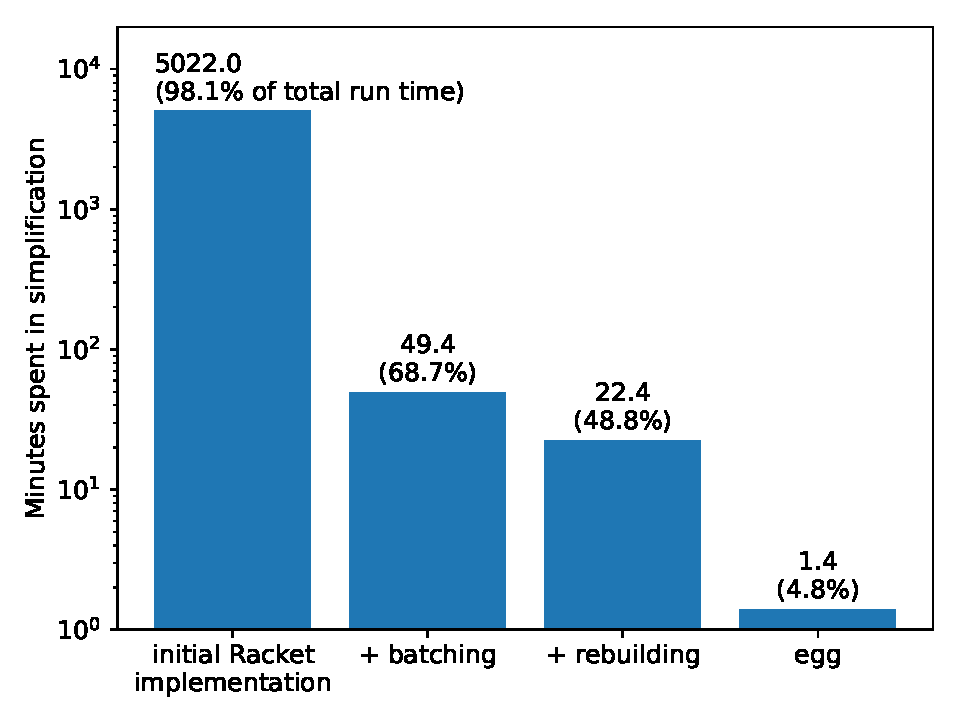
\includegraphics[height=5.5cm]{herbie}
  \caption{
    % Herbie sped up its expression simplification phase
    %   by adopting \egg-inspired features like
    %   batched simplification and rebuilding
    %   into its Racket-based \egraph implementation.
    % Herbie also supports using \egg itself for additional speedup.
    % Note that the y-axis is log-scale.
    Herbie 通过在 基于 Racket 的 \egraph 实现中采用像批量简化和重建这样的 \egg 启发式特性,% ?
      来加速其表达式简化阶段。
    Herbie 还支持使用 \egg 本身来获得额外的加速。
    注意 y 轴是对数刻度。
  }
  \label{fig:herbie-results}
\end{figure}


% Our \egg simplification backend
%   is a drop-in replacement to the existing Herbie simplifier,
%   making it easy to compare speed and results.
% We compare using
%   Herbie's standard test suite of roughly 500 benchmarks,
%   with timeouts disabled.
% \autoref{fig:herbie-results} shows the results.
% The \egg simplification backend is over
%   $3000\times$ faster than Herbie's initial simplifier.
% This speedup eliminated Herbie's largest bottleneck:
%   the initial implementation dominated Herbie's total run time at $98.1\%$,
%   backporting \egg improvements into Herbie cuts
%   that to about half the total run time,
%   and \egg simplification takes under $5\%$ of the total run time.
% Practically, the run time of Herbie's initial implementation was smaller, since
%   timeouts cause tests failures when simplification takes too long.
% Therefore, the speedup also improved Herbie's completeness,
%   as simplification now never times out.
\egg 简化器后端是现有 Herbie 简化器的插入式替代品(drop-in replacement),
  使比较速度和结果变得容易。
我们使用 Herbie 的标准测试套件,大约有500个基准测试,其中禁用了超时。
\autoref{fig:herbie-results} 显示了测试结果。
\egg 简化后端比 Herbie 的初始简化器快了 $3000\times$。
这种加速消除了 Herbie 的最大瓶颈:
  原始实现占 Herbie 总运行时间的 $98.1\%$,
  将 \egg 改进移植到 Herbie 中将其减少到总运行时间的一半,
  \egg 简化器占总运行时间的不到 $5\%$ 。
实际上,Herbie 初始实现的运行时间更短,因为超时会导致简化时间过长时测试失败。
因此加速也提高了 Herbie 的完备性,因为简化过程现在永远不会超时,。


% Since incorporating \egg into Herbie, the Herbie developers have backported some
%   of \egg's key performance improvements into the Racket \egraph implementation.
% First, batch simplification gives a large speedup because Herbie simplifies many
%   similar expressions.
% When done simultaneously in one equality saturation, the \egraph's structural
%   sharing can massively deduplicate work.
% Second, deferring rebuilding (as discussed in \autoref{sec:rebuilding}) gives a
%   further $2.2\times$ speedup.
% As demonstrated in \autoref{fig:eval-iter}, rebuilding offers an asymptotic
%   speedup, so Herbie's improved implementation (and the \egg backend as well)
%   will scale better as the search size grows.
自从将 \egg 纳入 Herbie 以来,Herbie 开发人员已经将一些
  \egg 的关键性能改进移植到了 Racket \egraph 实现中。
首先,批量简化给出了很大的加速,因为 Herbie 简化了许多相似的表达式。
在一个 等式饱和 的同时进行时,\egraph 的结构共享可以大量地减少重复工作。
其次,推迟重建 (如 \autoref{sec:rebuilding} 中所述) 给出了进一步的 $2.2\times$ 加速。
如 \autoref{fig:eval-iter} 所示,重建提供了渐近
  加速,因此 Herbie 的改进实现 (以及 \egg 后端)
  将随着搜索规模的增长而更好地扩展(scale)。 % ?scale

% \subsection{Spores: Optimizing Linear Algebra}
\subsection{Spores: 优化线性代数}
\label{sec:spores}


% Spores \cite{spores} is an optimizer for machine learning programs. It
% translates linear algebra (LA) expressions to relational algebra (RA), performs
% rewrites, and finally translates the result back to linear algebra. Each rewrite
% is built up from simple identities in relational algebra like the associativity
% of join. These relational identities express more fine-grained equality than
% textbook linear algebra identities, allowing Spores to discover novel
% optimizations not found by traditional optimizers based on LA identities. Spores
% performs holistic optimization, taking into account the complex interactions
% among factors like sparsity, common subexpressions, and fusible operators and
% their impact on execution time.
Spores \cite{spores} 是一个机器学习程序的优化器。
它将线性代数(LA)表达式翻译成关系代数(RA),进行重写,最后将结果再翻译成线性代数。
每一次重写都是由关系代数中的简单特性建立起来的,比如连接的关联性。
与教科书上的线性代数特性相比,这些关系特性表达了更精细的平等性,
使得 Spores 能够发现传统优化器基于 LA 特性所不能发现的新型优化。
Spores 进行整体优化(holistic optimization),
考虑到诸如稀疏性、共同子表达式和可融合运算符等因素之间复杂的相互作用以及它们对执行时间的影响。


% \Max{we should probably tone down some of the language below}

% \subsubsection{Implementation}
\subsubsection{实现}
% \Max{don't say ``we''}


% Spores is implemented entirely in Rust using \Egg.
% \Egg empowers Spores to orchestrate
%   the complex interactions described above elegantly and effortlessly.
% Spores works in three steps: first, it translates the input LA expression to RA;
% second, it optimizes the RA expression by equality saturation; finally, it
% translates the optimized RA expression back to LA.
Spores 完全用 Rust 和 \Egg 实现。
\Egg 赋予 Spores 优雅而轻松地编排上述复杂交互。
Spores 工作三个步骤:首先,它将输入的 LA 表达式转换为 RA;
其次,它通过 等式饱和 优化 RA 表达式;最后,它
将优化后的 RA 表达式转换回 LA。
% Since the translation between LA and RA is
% straightforward, we focus the discussion on the equality saturation step in RA.
% Spores represents a relation as a function from tuples to real numbers: $A:
% (a_1, a_2, ..., a_n) \rightarrow \mathbb{R}$. This is similar to the index
% notation in linear algebra, where a matrix A can be viewed as a function
% $\lambda i, j . A_{ij}$. A tuple is identified with a named record,
% e.g. $(1, 2) = \{a_1: 1, a_2: 2\} = \{a_2: 2, a_1: 1\}$, so that order in a
% tuple doesn't matter. There are just three operations on relations: join, union
% and aggregate. Join ($\otimes$) takes two relations and returns their natural
% join, multiplying the associated real number for joined tuples:
由于 LA 和 RA 之间的转换是直接的,因此我们将讨论集中在 RA 中的 等式饱和 步骤上。
Spores 将关系表示为从元组到实数的函数: 
$A: (a_1, a_2, ..., a_n) \rightarrow \mathbb{R}$。
这类似于线性代数中的索引符号,其中矩阵 A 可以被视为函数 
$\lambda i, j . A_{ij}$。
元组与命名记录相同,例如 $(1, 2) = \{a_1: 1, a_2: 2\} = \{a_2: 2, a_1: 1\}$,
因此元组中的顺序无关紧要。关系上只有三种操作: join, union 和 aggregate。 
Join ($\otimes$) 接受两个关系并返回它们的自然 join,将连接元组的关联实数相乘:
\[ A \otimes B = \lambda \bar{a} \cup \bar{b} . A(\bar{a}) \times B(\bar{b})\]
% 此段翻译未仔细校对
% Here $\bar{a}$ is the set of field names for the records in $A$. In RA
% terminology, $\bar{a}$ is the {\em schema} of $A$. Union ($\oplus$) is a join in
% disguise: it also performs natural join on its two arguments, but adds the
% associated real instead of multiplying it:
这里 $\bar{a}$ 是 $A$ 中记录的字段名集合。
在 RA 术语中,$\bar{a}$ 是 $A$ 的 {\em schema}。
Union ($\oplus$) 是一种伪装的 join:它在其两个参数上也执行自然 join,但是添加而不是乘以关联实数:
\[A \oplus B = \lambda \bar{a} \cup \bar{b} . A(\bar{a}) + B(\bar{b})\] 
% Finally, aggregate ($\Sigma$) sums its argument along a given dimension. It
% coincides precisely with the ``sigma notation'' in mathematics:
最后, aggregate($\Sigma$) 沿给定维度求和其参数。它与数学中的“sigma 符号”完全相同:
\[\sum_{a_i} A = \lambda \bar{a}-a_i . \sum_{a_i} A(\bar{a})\]

% \begin{figure}
% \centering
% \begin{align}
%   \label{eq:RRC_pp} A \oplus (B \oplus C) &= \oplus (A, B, C)
%   & \text{($\oplus$ is assoc. \& comm.)}
%   \\
%   \label{eq:RRC_mm} A \otimes (B \otimes C) &= \otimes (A, B, C)
%   & \text{($\otimes$ is assoc. \& comm.)}
%   \\
%   \label{eq:RRC_mp} A \otimes (B \oplus C) &= A \otimes B \oplus A \otimes C
%   & \text{($\otimes$ distributes over $\oplus$)}
%   \\
%   \label{eq:RRC_ap} \sum_i (A \oplus B) &= \sum_i A \oplus \sum_i B
%   \\
%   \label{eq:RRC_aa} \sum_i \sum_j A &= \sum_{i,j} A
%   \\
%   \label{eq:RRC_ma} A \otimes \sum_i B &= \sum_i (A \otimes B)
%   &\text{(requires $i \not\in A$)}
%   \\
%   \label{eq:RRC_ac} \sum_i A &= A \otimes \textsf{dimension}(i)
%   &\text{(requires $i \not\in A$)}
% \end{align}
% % \caption{RA equality rules $R_{EQ}$.}
% \caption{RA 等式规则~$R_{EQ}$.}
% \label{fig:RRC}
% \end{figure}
\begin{figure}
\centering
\begin{align}
  \label{eq:RRC_pp} A \oplus (B \oplus C) &= \oplus (A, B, C)
  & \text{($\oplus$ 满足结合律 \& 交换律)}
  \\
  \label{eq:RRC_mm} A \otimes (B \otimes C) &= \otimes (A, B, C)
  & \text{($\otimes$ 满足结合律 \& 交换律)}
  \\
  \label{eq:RRC_mp} A \otimes (B \oplus C) &= A \otimes B \oplus A \otimes C
  & \text{($\otimes$ 对于 $\oplus$ 满足分配率)}
  \\
  \label{eq:RRC_ap} \sum_i (A \oplus B) &= \sum_i A \oplus \sum_i B
  \\
  \label{eq:RRC_aa} \sum_i \sum_j A &= \sum_{i,j} A
  \\
  \label{eq:RRC_ma} A \otimes \sum_i B &= \sum_i (A \otimes B)
  &\text{(要求 $i \not\in A$)}
  \\
  \label{eq:RRC_ac} \sum_i A &= A \otimes \textsf{dimension}(i)
  &\text{(要求 $i \not\in A$)}
\end{align}
% \caption{RA equality rules $R_{EQ}$.}
\caption{RA 等式规则 $R_{EQ}$.}
\label{fig:RRC}
\end{figure}


% 此段翻译未仔细校对
% The RA identities, presented in \autoref{fig:RRC}, are also simple and intuitive.
% The notation $i \not\in A$ means $i$ is not in the schema of $A$, and $dim(i)$
% is the size of dimension $i$ (e.g. length of rows in a matrix). In
% \autoref{eq:RRC_ma}, when $i \in A$, we first rename every $i$ to a fresh variable
% $i'$ in $B$, which gives us: $A \otimes \sum_i B = \sum_{i'} (A \otimes B[i
% \rightarrow i'])$. In addition to these equalities, Spores also supports
% replacing expressions with fused operators. For example, $(X-UV)^2$ can be
% replaced by $sqloss(X, U, V)$ which streams values from $X, U, V$ and
% computes the result without creating intermediate matrices. Each of these fused
% operators is encoded with a simple identity in \Egg.
在 \autoref{fig:RRC} 中呈现的 RA 指示器(identities)也是简单直观的。 %?RA identities
符号$i \not\in A$ 表示 $i$ 不在 $A$ 的模式中,
  $dim(i)$ 是维度 $i$ 的大小(例如,矩阵中的行长度)。
在\autoref{eq:RRC_ma} 中,当$i \in A$ 时,我们首先将$i$重命名为$B$中的新变量$i'$,
  这给我们:$A \otimes \sum_i B = \sum_{i'} (A \otimes B[i \rightarrow i'])$。
除了这些等式之外,Spores 还支持用融合运算符替换表达式。
例如,$(X-UV)^2$ 可以用 $sqloss(X, U, V)$ 替换,
这将从 $X, U, V$ 中流式传输值并在不创建中间矩阵的情况下计算结果。
这些融合运算符中的每一个都在 \Egg 中以简单身份编码。

% 此段翻译未仔细校对
% Note that \autoref{eq:RRC_ma} requires a way
% to store the schema of every expression during optimization.
% Spores uses an \eclass analysis to annotate \eclasses with the appropriate
%   schema. It also leverages the \eclass analysis for cost estimation,
%   using a conservative cost model that overapproximates.
% As a result, equivalent expressions may have different cost estimates.
% The \texttt{merge} operation on the analysis data takes the lower cost,
%   incrementally improving the cost estimate.
% Finally, Spores' \eclass analysis also performs constant folding.
% As a whole, the \eclass analysis is a composition of three smaller analyses
%   in a similar style to the composition of lattices in abstract interpretation.
注意,在优化过程中,\autoref{eq:RRC_ma} 需要存储每个表达式的模式。
Spores 使用 \eclass 分析来为 \eclasses 注释适当的模式,
  它还利用\eclass 分析进行成本估算,使用过高估计的保守成本模型。
因此,等价的表达式可能具有不同的成本估计。
  对分析数据的 \texttt{merge} 操作采用较低的成本,逐渐改善成本估计。
最后,Spores的 \eclass 分析还执行常量折叠。
总之,\eclass 分析是三个较小分析的组合,
  类似于抽象解释中的格点(lattices)组合。% ? composition of lattices

% \subsubsection{Results}
\subsubsection{评估}

% Spores is integrated into Apache SystemML \cite{Boehm_2019} in a prototype,
% where it is able to derive all of 84 hand-written rules and heuristics for
% sum-product optimization. It also discovered novel rewrites that contribute
% to $1.2\times$ to $5\times$ speedup in end-to-end experiments. With greedy
% extraction, all compilations completed within a second.
Spores 已被集成到 Apache SystemML \cite{Boehm_2019} 的原型中,
在那里它能够推导出 84 个手写的规则(hand-written rules)和启发式算法来进行和积优化。
它还发现了新的重写,在端到端实验中贡献了 $1.2\times$ 到 $5\times$ 的加速。
使用贪心提取(greedy extraction),所有编译能都在一秒钟内完成。 %?greedy extraction


% \subsection{Szalinski: Decompiling CAD into Structured Programs}
\subsection{Szalinski: 将 CAD 反编译为结构化程序}
\label{sec:szalinski}

% \begin{figure}
%   \centering
%   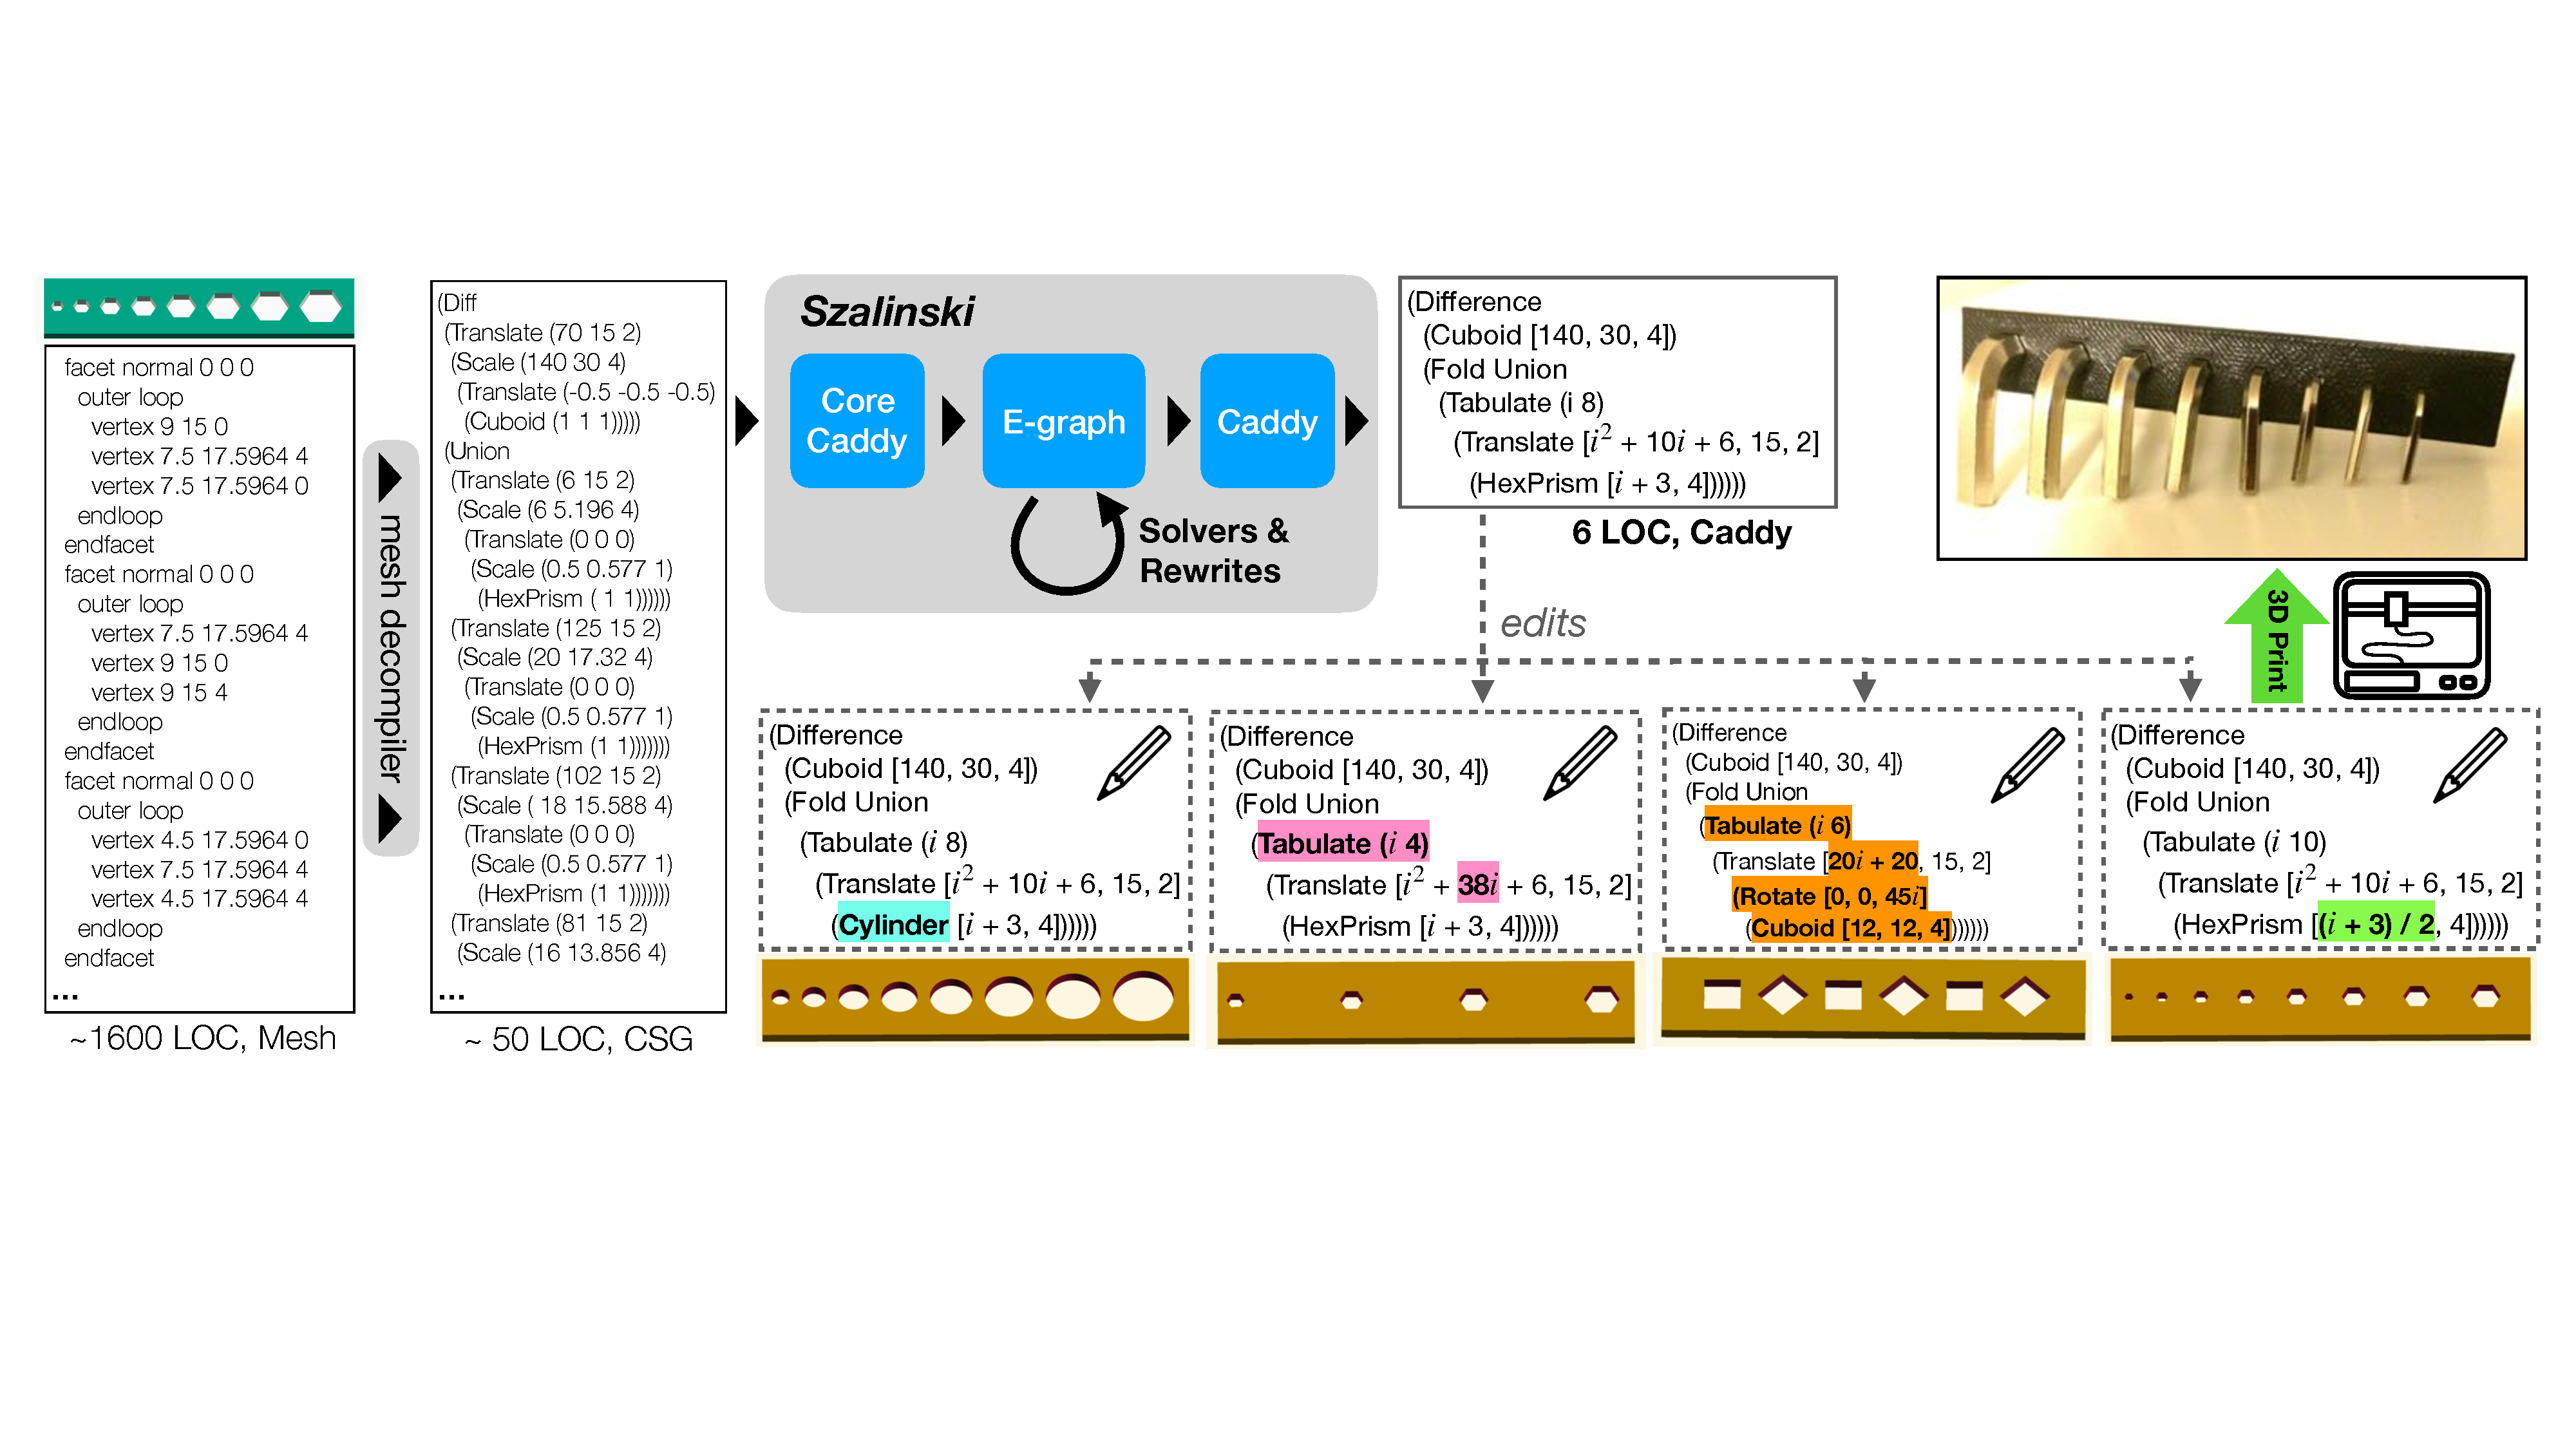
\includegraphics[width=\linewidth]{sz-overview}
%   \caption[Szalinski decompiles flat CSG into structured CAD]{
%   (Figure from Nandi et.\ al.\ \cite{szalinski})
%   Existing mesh decompilers turn
%     triangle meshes into flat, computational solid geometry (CSG) expressions.
%   %  The size of both mesh and CSG are roughly proportional to
%   %    the number of geometric features in the CAD model.
%   \sz~\cite{szalinski} takes in these CSG expressions
%     in a format called Core Caddy,
%     and it synthesizes smaller, structured programs in language called Caddy
%     that is enriched with functional-style features.
%   This can ease customization by simplifying edits:
%     small, mostly local changes
%     yield usefully different models.
%   The photo shows the 3D printed hex wrench holder after
%     customizing hole sizes.
%   \sz is powered by \egg's extensible equality saturation, relying on its high
%     performance, \eclass analyses, and dynamic rewrites.
%   }
%   \label{fig:sz-overview}
% \end{figure}
\begin{figure}
  \centering
  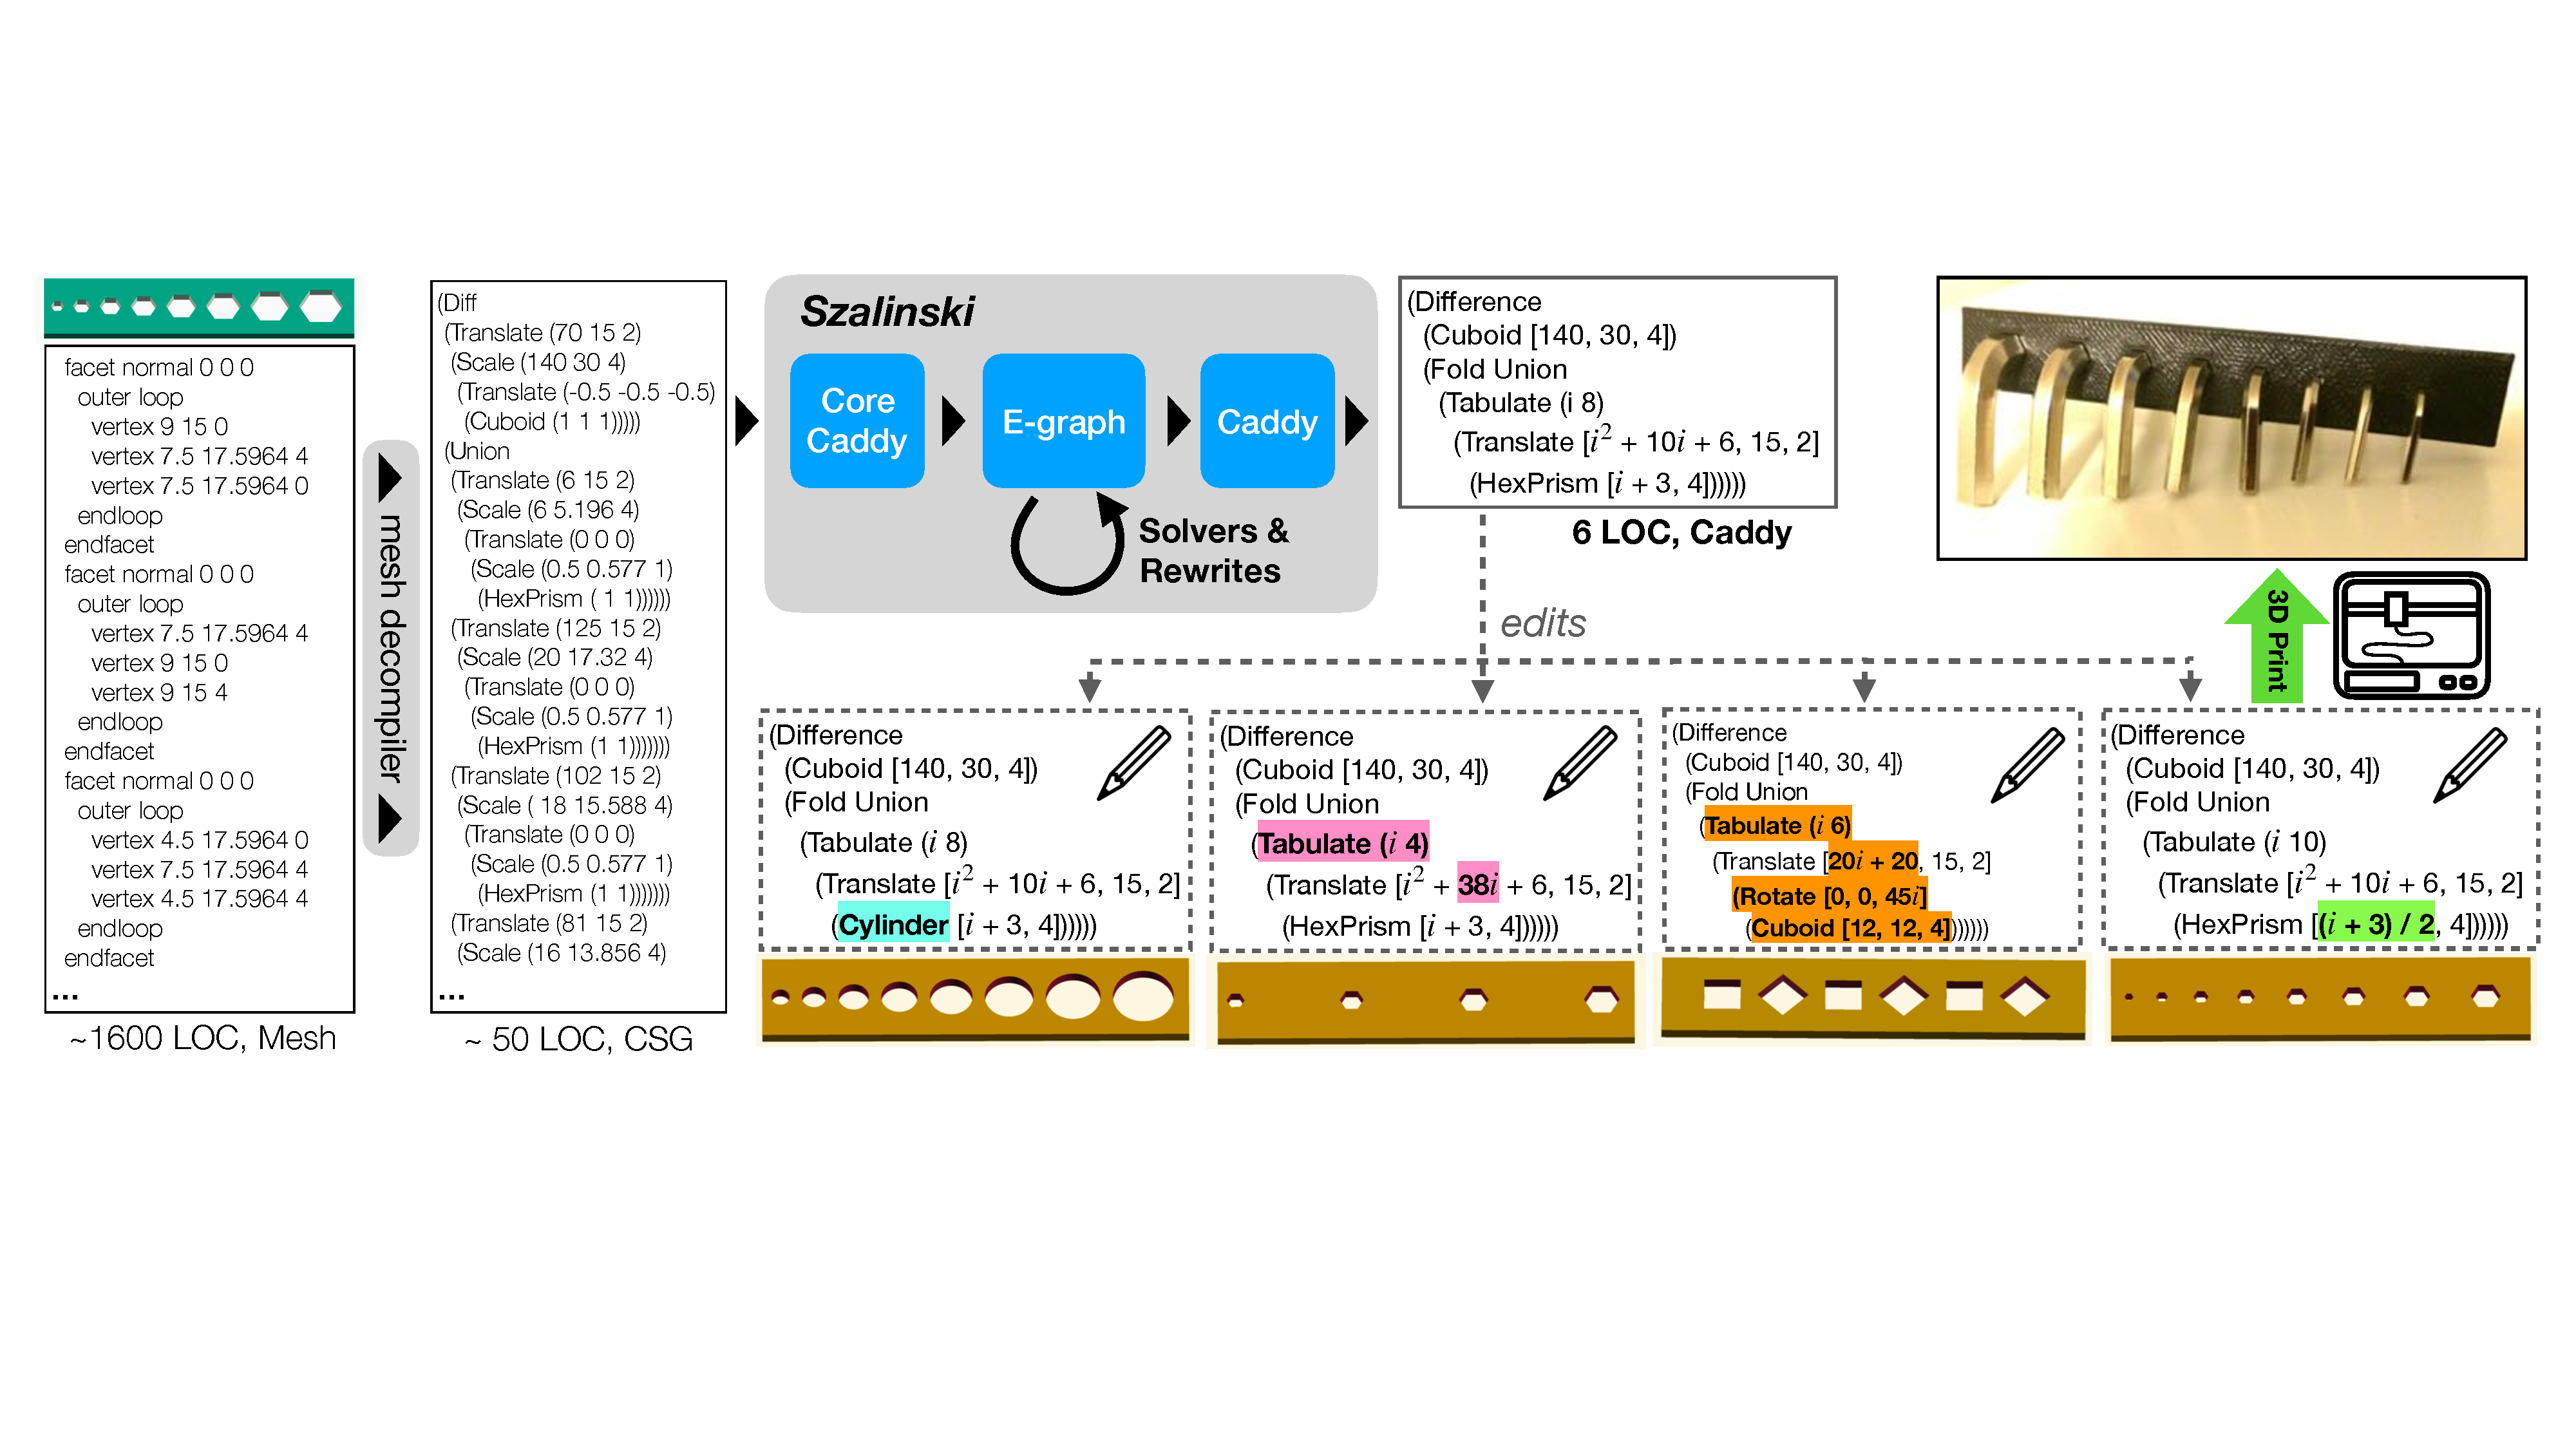
\includegraphics[width=\linewidth]{sz-overview}
  \caption[Szalinski decompiles flat CSG into structured CAD]{
  (图源自 Nandi et.\ al.\ \cite{szalinski})
  现有的网格反编译器(mesh decompiler)将三角网格转换为平面的计算固体几何(CSG)表达式。
  \sz~\cite{szalinski} 在一种称为 Core Caddy 的格式中输入这些 CSG 表达式,
    基于 Caddy 语言综合(synthesizes)了更小的、结构化的程序,它具有函数式编程的特性。 
    % 综合 synthesizes 这个翻译来自于《形式化方法概貌》
    这可以通过简化编辑来简化定制:
      小的、主要是局部更改,来产生有用的不同模型。
    照片展示了定制孔尺寸后 3D 打印的六角扳手架。
    \sz 是基于 \egg 高性能、\eclass 分析和动态重写的可扩展 等式饱和 驱动的。
  }
  \label{fig:sz-overview}
\end{figure}


% Several tools have emerged
%   that reverse engineer high level
%   Computer Aided Design (CAD) models from polygon
%   meshes and voxels~\cite{reincarnate, inverse, shape, csgnet, latex}.
% The output of these tools are constructive solid geometry (CSG) programs.
% A CSG program is comprised of
%   3D solids like cubes, spheres, cylinders,
%   affine transformations like scale, translate, rotate
%   (which take a 3D vector and a CSG expression as arguments),
%   and binary operators like union, intersection, and difference
%   that combine CSG expressions.
% For repetitive models like a gear, CSG programs can be too long
%   and therefore difficult to comprehend.
% A recent tool, \sz~\cite{szalinski},
%   extracts the inherent structure
%   in the CSG outputs of mesh decompilation tools
%   by automatically inferring maps and folds (\autoref{fig:sz-overview}).
% \sz accomplished this using \egg's extensible equality saturation system,
%   allowing it to:
目前已有几种工具可以从多边形网格和体素中逆向 CAD(高级计算机辅助设计,Computer Aided Design)模型
  ~\cite{reincarnate, inverse, shape, csgnet, latex}。
这些工具的输出是构造实体几何(CSG)程序。
一个 CSG 程序由 3D 实体如立方体、球体、圆柱体、仿射变换(如缩放、平移、旋转)
  和二元运算符如并集、交集和差集组成,它们结合了 CSG 表达式。
对于像齿轮这样的重复模型,CSG 程序可能太长,因此难以理解。
一个近来的工具, \sz~\cite{szalinski} ,通过自动推断映射(maps)和折叠(folds)( \autoref{fig:sz-overview})
  ,可以在网格反编译(mesh decompilation)工具的 CSG 输出中提取固有结构。
\sz 通过 \egg 的可扩展 等式饱和 系统实现了这一目标:


\begin{itemize}

  % \item Discover structure using loop rerolling rules.
  %   This allows \sz to infer functional patterns like
  %   \texttt{Fold}, \texttt{Map2}, \texttt{Repeat} and
  %   \texttt{Tabulate} from flat CSG inputs.
  \item 使用循环重投(loop rerolling)规则发现结构。
    这使得\sz 能够从平面CSG输入中推断出
    \texttt{Fold}, \texttt{Map2}, \texttt{Repeat} 和 \texttt{Tabulate} 
    等函数模式。

  % \item Identify equivalence among CAD terms that are
  %   expressed as different expressions by mesh decompilers.
  %   \sz accomplishes this by using CAD identities.
  %   An example of one such CAD identity in \sz is
  %   $e \leftrightarrow \mathit{rotate}~[0 ~ 0 ~ 0] ~ e$.
  %   This implies that any CAD expression $e$
  %   is equivalent to a CAD expression that applies
  %   a rotation by zero degrees about x, y, and z axes
  %   to $e$.
  \item 识别由网格解压器表示为不同表达式的 CAD 术语之间的等价性。
    \sz 通过使用 CAD id (CAD identities)来实现这一点。
    \sz 中的一个 CAD id 示例是
    $e \leftrightarrow \mathit{rotate}~[0 ~ 0 ~ 0] ~ e$。
    这意味着任何 CAD 表达式 $e$ 等价于对 $e$ 应用 x, y, z 轴上零度旋转的 CAD 表达式。

  % \item Use external solvers to
  %   speculatively add potentially profitable
  %   expressions to the \egraph.
  %   Mesh decompilers often generate CSG expressions
  %   that order and/or group list elements in
  %   non-intuitive ways.
  %   To recover structure from such expressions,
  %   a tool like \sz must be able to reorder and regroup
  %   lists that expose any latent structure.
  \item 使用外部求解器向 \egraph 中添加可能有利可图的表达式。
    网格解压器经常生成以非直观方式排序和/或分组列表元素的 CSG 表达式。
    为了从这样的表达式中恢复结构,\sz 这样的工具必须能够重新排序和重新分组列表,暴露任何潜在结构。

\end{itemize}

% \subsubsection{Implementation}
\subsubsection{实现}


% Even though CAD is
%   different from traditional languages
%   targeted by programming language techniques,
%   \egg supports \sz's CAD language in a straightforward manner.
% \sz uses purely syntactic rewrites to express
%   CAD identities and some loop rerolling rules
%   (like inferring a \texttt{Fold} from a list of CAD expressions).
% Critically, however, \sz relies on \egg's
%   dynamic rewrites and \eclass analysis to infer functions
%   for lists.
尽管 CAD 与编程语言技术针对的传统语言不同,但是 \egg 以直接的方式支持 \sz 的 CAD 语言。
\sz 使用纯语法重写来表示 CAD 身份和一些循环重绕规则
  (如从 CAD 表达式列表推断出 \texttt{Fold} )。
然而关键的是,\sz 依赖于 \egg 的动态重写和 \eclass 分析来推断列表的函数。

% 此段翻译未仔细校对
% Consider the flat CSG program in \autoref{fig:sz-egg-input}.
% A structure finding rewrite first rewrites the flat list of \texttt{Union}s to:
% $$\texttt{(Fold Union (Map2 Translate [(0 0 0) (2 0 0) ...] (Repeat Cube 5)))}$$
% The list of vectors is stored as \texttt{Cons} elements (sugared above for brevity).
% \sz uses an \eclass analysis to track the accumulated lists in a similar style
%   to constant folding.
% Then, a dynamic rewrite uses an arithmetic solver to rewrite the concrete
%   list of 3D vectors in the analysis data
%   to \mbox{\texttt{(Tabulate (i 5) (* 2 i))}}.
% A final set of syntactic rewrites can hoist the \texttt{Tabulate}, yielding the
%   result on the right of \autoref{fig:sz-egg}.
% Thanks to the set of syntactic CAD rewrites, this structure finding even works
%   in the face of CAD identities.
% For example, the original program may omit the no-op
%   \texttt{Translate (0 0 0)}, even though it is necessary to see repetitive
%   structure.
考虑 \autoref{fig:sz-egg-input} 中的平面 CSG 程序。
结构发现重写首先将平面的 \texttt{Union} 列表重写为:
$$\texttt{(Fold Union (Map2 Translate [(0 0 0) (2 0 0) ...] (Repeat Cube 5)))}$$
向量列表存储为 \texttt{Cons} 元素(上面简化了)。
\sz 使用 \eclass 分析来跟踪累积列表,类似于常量折叠。
然后,动态重写使用算术求解器重写分析数据中的具体 3D 向量列表,
  以 \mbox{\texttt{(Tabulate (i 5) (* 2 i))}} 的形式。
最后一组语法重写可以提升(hoist) \texttt{Tabulate},得到 \autoref{fig:sz-egg} 右侧的结果。
由于一系列 CAD 语法 重写的存在,即使面对 CAD id,这种结构发现也能正常工作。
例如,原始程序可能省略无操作的 \texttt{Translate (0 0 0)},即使它是观察重复结构所必需的。

\begin{figure}
\begin{subfigure}[b]{0.3\linewidth}
  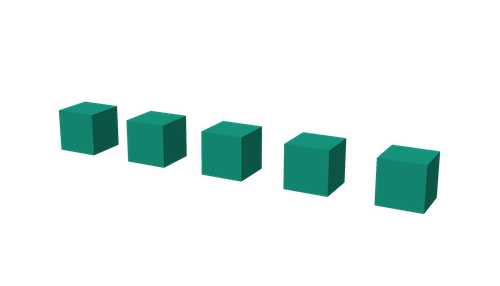
\includegraphics[width=\linewidth]{cubes}
  % \caption{Five cubes in a line.}
  \caption{一条线中的五个立方体。}
\end{subfigure}
\hfill
\begin{subfigure}[b]{0.3\linewidth}
  \begin{lstlisting}[language=Rust, gobble=4, basicstyle=\footnotesize\ttfamily]
    (Union
      (Translate (0 0 0) Cube)
      (Translate (2 0 0) Cube)
      (Translate (4 0 0) Cube)
      (Translate (6 0 0) Cube)
      (Translate (8 0 0) Cube))
  \end{lstlisting}
  % \caption{Flat CSG input to \sz.}
  \caption{Flat CSG 输入到 \sz。}
  \label{fig:sz-egg-input}
\end{subfigure}
\hfill
\begin{subfigure}[b]{0.35\linewidth}
  \begin{lstlisting}[language=Rust, gobble=4, basicstyle=\footnotesize\ttfamily, showlines=true, xleftmargin=5mm]
    (Fold Union
      (Tabulate (i 5)
        (Translate
          ((* 2 i) 0 0)
          Cube)))

  \end{lstlisting}
  % \caption{Output captures the repetition.}
  \caption{输出捕获了重复。}
  \label{fig:sz-egg-output}
\end{subfigure}
  \caption{
    % \sz integrates solvers into \egg's equality saturation as a dynamic rewrite.
    % The solver-backed rewrites can transform repetitive lists into
    % \texttt{Tabulate} expressions that capture the repetitive structure.
    \sz 将求解器作为动态重写集成到 \egg 的 等式饱和 中。
    支持求解器的重写可以将重复列表转换为捕获重复结构的 \texttt{Tabulate} 表达式。%?solver-backed
  }
  \label{fig:sz-egg}
\end{figure}


% In many cases, the repetitive structure of input CSG expression is further
%   obfuscated because subexpressions may appear in arbitrary order.
% For these inputs, the arithmetic solvers must first reorder
%   the expressions to find a closed form like a \texttt{Tabulate}
%   as shown in \autoref{fig:sz-egg}.
% However, reordering a list does not preserve equivalence, so adding it to the
%   \eclass of the concrete list would be unsound.
% \sz therefore introduces \textit{inverse transformations},
%   a novel technique that allows solvers to speculatively reorder and regroup list
%   elements to find a closed form.
% The solvers annotate the potentially profitable expression with the
%   permutation or grouping that led to the successful discovery
%   of the closed form.
% Later in the rewriting process, syntactic rewrites eliminate the inverse
%   transformations when possible
%   (e.g., reordering lists under a \texttt{Fold Union} can be eliminated).
% \egg supported this novel technique without modification.
在很多情况下,输入 CSG 表达式的重复结构进一步混淆,因为子表达式可能以任意顺序出现。
对于这些输入,算术求解器必须首先重新排序表达式,以找到像 \texttt{Tabulate} 这样的封闭形式,如 \autoref{fig:sz-egg} 所示。然
而,重新排序列表不会保留等价性,因此将其添加到具体列表的 \eclass 中将是不安全的。
因此,\sz 引入了新技术 \textit{反向变换(inverse transformations)},
  允许求解器推测重新排序和重新分组列表元素以找到封闭形式。求解器使用导致成功发现封闭形式的排列或分组注释可能有利可图的表达式。
在重写过程的后期,语法重写在可能时删除反向变换
  (例如,在\texttt{Fold Union} 下重新排序列表可以被删除)。
\egg 支持了这种新颖的技术,而无需修改。

% \subsubsection{Results}
\subsubsection{评估}

% \sz's initial protoype used a custom \egraph written in OCaml.
% Anecdotally, switching to \egg
%   removed most of the code,
%   eliminated bugs,
%   facilitated the key contributions of solver-backed rewrites and inverse transformations,
%   and made the tool about $1000 \times$ faster.
% \egg's performance allowed a shift from running on small, hand-picked
%   examples to a comprehensive evaluation on over 2000 real-world models from
%   a 3D model sharing forum~\cite{szalinski}.
\sz 的初始原型使用 OCaml 编写的自定义 \egraph。
有趣的是,使用 \egg 删除了大部分代码,
  消除了错误,
  促进了求解器支持的重写(solver-backed rewrites)和反向变换(inverse transformations)
  的关键贡献, 
  并使工具快了约 $1000 \times$。
\egg 的性能允许从运行小型手工选择的示例转变为对来自 3D 模型共享论坛~\cite{szalinski}
  的 2000 多个真实世界模型的综合评估。


%%% Local Variables:
%%% TeX-master: "egg"
%%% End:

% numbering break, these must come last
\section{相关工作}
% \section{Related Work}
\label{sec:related}
% 草草翻译完成

% \paragraph{Term Rewriting}
\paragraph{Term 重写}

% 此段翻译未仔细校对 :-( 
% Term rewriting~\cite{rewritesystems} has been used widely to facilitate
% equational reasoning for program
% optimizations~\cite{DBLP:conf/scitools/BoyleHW96,
%   DBLP:journals/toplas/BrandHKO02, DBLP:conf/icfp/VisserBT98}. A term rewriting
% system applies a database of semantics preserving rewrites or axioms to an input
% expression to get a new expression, which may, according to some cost function,
% be more profitable compared to the input. Rewrites are typically symbolic and
% have a left hand side and a right hand side. To apply a rewrite to an
% expression, a rewrite system implements pattern matching---if the left hand side
% of a rewrite rule matches with the input expression, the system computes a
% substitution which is then applied to the right-hand side of the rewrite rule.
% Upon applying a rewrite rule, a rewrite system typically replaces the old
% expression by the new expression. This can lead to the \textit{phase ordering}
% problem--- it makes it impossible to apply a rewrite to the old expression in
% the future which could have led to a more optimal result. 
Term 重写~\cite{rewritesystems} 已被广泛用于促进程序优化~\cite{DBLP:conf/scitools/BoyleHW96,
  DBLP:journals/toplas/BrandHKO02, DBLP:conf/icfp/VisserBT98}的等式推理中。
Term 重写系统将保留语义的重写或公理的数据库应用于输入表达式,
  以得到一个新的表达式,根据一些成本函数,这个表达式与输入式相比可能更有利。
  重写通常是符号化的,有一个左式和一个右式。
  为了对一个表达式进行重写,重写系统实现了模式匹配
  ——如果重写规则的左侧与输入表达式相匹配,系统就会计算出一个替换,然后应用到重写规则的右侧。
  在应用重写规则时,重写系统通常会用新的表达式替换旧的表达式。
  这可能会导致 \textit{阶段排序(phase ordering)} 的问题
  —— 它使得在未来不可能对旧的表达式进行重写,而这可能会导致更优的结果。


% \paragraph{\Egraphs and E-matching}
\paragraph{\Egraphs 和 E-matching}

% 此段翻译未仔细校对 :-( 
% \Egraph were originally proposed several decades ago as an
% efficient data structure for maintaining congruence
% closure~\cite{nelson-oppen-78, kozen-stoc77, nelson}.
% \Egraphs continue to be a critical component in successful SMT
% solvers where they are used for combining satisfiability theories by sharing equality
% information~\cite{z3}.
%  A key difference between past implementations of \egraphs and
%   \egg's \egraph is our novel rebuilding algorithm that maintains
%   invariants only at certain critical points~(\autoref{sec:rebuild}).
% This makes \egg more efficient for the purpose of equality saturation.
%   \egg implements the pattern compilation strategy introduced by de Moura et al.~\cite{ematching}
%   that is used in state of the art theorem provers~\cite{z3}.
\Egraph 最初是几十年前提出的一种高效的数据结构,
  用于维护同余闭包~\cite{nelson-oppen-78, kozen-stoc77, nelson}。
\Egraphs 仍然是成功的 SMT 求解器中的关键组成部分,
  它们被用于通过共享等价关系结合可满足性理论~\cite{z3}。 % ?
过去 \egraph 实现和 \egg 的 \egraph 的主要区别在于我们新颖的重建算法——
  只在某些关键点维护不变性~(\autoref{sec:rebuild})。
这使得 \egg 更适合等价饱和的目的。
\egg 实现了 de Moura 等人提出的模式编译策略~\cite{ematching},
  该策略在最先进的定理证明器~\cite{z3}中使用。
% Some provers~\cite{z3, simplify} propose optimizations like mod-time,
% pattern-element and inverted-path-index to find new terms and relevant patterns
% for matching, and avoid redundant matches. So far, we have found \egg to be
% faster than several prior \egraph implementations even without
% these optimizations. They are,
% however, compatible with \egg's design and could be explored in the future. Another
% key difference is \egg's powerful \eclass analysis abstraction and flexible
% interface. They empower the programmer to easily leverage \egraphs for problems
% involving complex semantic reasoning.
一些证明器~\cite{z3, simplify} 提出了像 
  mod-time,pattern-element 和 inverted-path-index 这样的优化,
  用于找到新的术语和相关模式进行匹配,避免重复匹配。
  到目前为止,我们发现 \egg 比之前的几个 \egraph 实现更快,即使没有这些优化。
然而,它们与 \egg 的设计兼容,可以在未来进行探索。
  另一个关键差异是 \egg 强大的 \eclass 分析抽象和灵活的界面。
  它们使程序员能够轻松地利用 \egraph 解决涉及复杂语义推理的问题。

% \paragraph{Congruence Closure}
\paragraph{同余闭包}

% 此段翻译未仔细校对 :-( 
% Our rebuilding algorithm is similar to the congruence closure algorithm
%   presented by \citet{downey-cse}.
% The contribution of rebuilding is not \emph{how} it restores the \egraph invariants
%   but \emph{when};
%   it gives the client the ability to specialize invariant restoration to a
%   particular workload like equality saturation.
% Their algorithm also features a worklist of merges to be processed further,
%   but it is offline, i.e.,
%   the algorithm processes a given set of equalities and outputs the set of
%   equalities closed over congruence.
% Rebuilding is adapted to the online e-graph (and equality saturation) setting,
%   where rewrites frequently examine the current set of equalities and assert new ones.
% Rebuilding additionally propagates e-class analysis facts (\autoref{sec:analysis}).
% Despite these differences,
%   the core algorithms algorithms are similar enough that theoretical results on
%   offline performance characteristics \cite{downey-cse} apply to both.
% We do not provide theoretical analysis of rebuilding for the online setting;
%   it is likely highly workload dependent.
我们的重建算法类似于 \citet{downey-cse} 提出的同余闭包(congruence closure)算法。
重建的贡献不在于它如何恢复 \egraph 不变性,而在于它什么时候恢复;
  客户端有能力将不变性恢复专门化为特定工作负载,如 等式饱和。
它的算法也具有要进一步处理的合并工作列表
  ,但它是离线的,即算法处理给定的等价关系并输出经过同构闭包的等价关系集。
重建适用于在线 e-graph(和等式饱和)设置,
  在这种设置中重写经常检查当前的等价关系并断言新的关系。
重建还传播 e-class 分析事实(\autoref{sec:analysis})。
尽管存在这些差异,但核心算法相似,离线性能特征 \cite{downey-cse} 适用于两者。
我们没有为在线设置提供重建的理论分析;它可能与工作负载高度相关。

% \paragraph{Superoptimization and Equality Saturation}
\paragraph{超优化(Superoptimization)~和~ 等式饱和}

% 此段翻译未仔细校对 :-( 
% The Denali~\cite{denali} superoptimizer first demonstrated how to use \egraphs
% for optimized code generation as an alternative to hand-optimized machine code
% and prior exhaustive approaches~\cite{massalin}, both of which were less
% scalable. The inputs to Denali are programs in a C-like language from which it
% produces assembly programs. Denali supported three types of
% rewrites---arithmetic, architectural, and program-specific. After applying these
% rewrites till saturation, it used architectural description of the hardware to
% generate constraints that were solved using a SAT solver to output a
% near-optimal program. While Denali's approach was a significant improvement over
% prior work, it was intended to be used on straight line code only and therefore,
% did not apply to large real programs.
Denali~\cite{denali} 超优化器首先展示了如何使用 \egraphs 进行优化代码生成,
作为手动优化机器代码和先前的详尽方法~\cite{massalin}的替代方案,两者都不易扩展。 
Denali 的输入是类 C 语言中的程序,它会生成汇编程序。 
Denali 支持三种重写——算术、架构和特定于程序。
在应用这些重写直到饱和之后,它使用硬件描述生成约束,使用 SAT 求解器解决这些约束以输出近似最优程序。
虽然 Denali 的方法比先前的工作有了重大改进,但它只适用于直线代码,因此不适用于大型实际程序。

% 此段翻译未仔细校对 :-( 
% Equality saturation~\cite{eqsat, eqsat-llvm} developed a compiler optimization
% phase that works for complex language constructs like loops and conditionals.
% The first equality saturation paper used an intermediate representation called
% Program Expression Graphs (PEGs) to encode loops and conditionals. PEGs have
% specialized nodes that can represent infinite sequences, which allows them to
% represent loops. It uses a global profitability heuristic for extraction which
% is implemented using a pseudo-boolean solver. Recently, \cite{yogo-pldi20} uses
% PEGs for code search.
% \egg can support PEGs as a user-defined language,
% and thus their technique could be ported.
等式饱和 ~\cite{eqsat, eqsat-llvm} 开发了编译优化选择算法,
适用于循环和条件等复杂语言结构。
第一篇关于等价饱和的论文使用中间表示,称为程序表达图(PEGs)来编码循环和条件。
PEGs 有专门的节点,可以表示无限序列,这样就可以表示循环。
它使用全局可盈利性启发式来进行提取,使用伪布尔求解器实现。
最近,\cite{yogo-pldi20} 使用 PEGs 进行代码搜索(code search)。
\egg 可以支持 PEGs 作为用户定义语言,因此它们的技术可以移植。


%PEGs could be implemented in \egg.

%%% Local Variables:
%%% TeX-master: "egg"
%%% End:

\section{总结}
% \section{Conclusion}
\label{sec:conclusion}
% 翻译完成

% We presented two new techniques,
%   rebuilding and \eclass analysis,
%   that make equality saturation
%   fast and extensible enough for a new family of
%   applications.
% Rebuilding is a new way to
%   amortize the cost of maintaining the \egraph's
%   data structure invariants,
%   specializing the \egraph to the equality saturation workload.
% \Eclass analysis is a general framework
%   %for lifting a form of abstract
%   %interpretation to the \egraph level,
%   allowing for interpreted reasoning
%   beyond what purely syntactic rewrites can provide.
我们提出了两种新技术,重建和 \eclass 分析,
  使得 等式饱和 变快且足够可扩展,可用于一类新的应用程序。
重建是一种新的方法,用于摊销维护 \egraph 数据结构不变性的成本,
  将 \egraph 针对 等式饱和 工作量来特化。 % ?
\eclass 分析是一个通用框架,可以提供超出纯语法重写所能提供的解释性推理。

% We implemented both of these techniques in \egg,
%   a reusable, extensible, and efficient \egraph library.
% \Egg is generic over the user-defined language,
%   which allowed focused effort on optimization and efficiency
%   while obviating the need for
%   ad hoc \egraph implementations and manipulations.
% Our case studies show that equality saturation can now scale
%   further and be used more flexibly than before;
%   \egg provided new functionality and large speedups.
% We believe that these contributions
%   position equality saturation as a powerful toolkit for
%   program synthesis and optimization.
我们在 \egg 中实现了这两种技术,\egg 是一个可重用、可扩展和高效的 \egraph 库。
\Egg 是针对用户定义语言的通用库,这使得我们能够专注于优化和效率,
  同时避免了临时性的 \egraph 实现和操作的需要。 % ? ad hoc
我们的案例研究表明, 等式饱和 现在可以进一步拓展,% ?scale further
  并比以前更灵活地使用;\egg 提供了新的功能和大幅性能加速。
我们相信这些贡献将 等式饱和 定位为程序合成和优化的的强大工具箱。

%%% Local Variables:
%%% TeX-master: "egg"
%%% End:


%\newpage
%\listoftodos[\textbf{TODOs}]\relax


\begin{acks}
  % Thanks to our anonymous paper and artifact reviewers for their feedback. 
  感谢我们的匿名论文和工件审稿人的反馈。
  % Special thanks to our shepherd Simon Peyton Jones,
  %   Leonardo de Moura,
  %   and many
  %   members of the \href{https://uwplse.org}{PLSE} group.
  特别感谢我们的指导人 Simon Peyton Jones, Leonardo de Moura, 
  和~\href{https://uwplse.org}{PLSE}~小组的许多成员。
  % This work was supported in part by
  %   the Applications Driving Architectures (ADA) Research Center,
  %   a JUMP Center co-sponsored by SRC and DARPA,
  %   as well as the National Science Foundation
  %   under Grant Nos. 1813166 and 1749570.
  这项工作得到了由 SRC 和 DARPA 共同赞助的 JUMP 中心的
    应用驱动体系结构(Applications Driving Architectures, ADA)研究中心的部分支持,
  以及 Grant Nos. 1813166 和 1749570 号国家科学基金会的支持。
\end{acks}


\bibliography{references}

\end{document}
